% Chapter 11: Spectral and wavelet analysis
% Advanced Time Series Analysis and Forecasting -- Master's programme Applied Statistics and Data Science, year 1, semester 2, Bucharest University of Economic Studies
% GENERATED by latex/build_chapter11.py -- edit the generator, not this file.

\newcommand{\coursename}{Advanced Time Series Analysis and Forecasting}
% Preambul comun ATS -- Analiza avansată a seriilor de timp și previziune / Advanced Time Series Analysis and Forecasting
% (Beamer, 16:9). Același design ca MFM, SFM și TSA (copiat din TSA, 5 octombrie 2026). Înainte de % Preambul comun ATS -- Analiza avansată a seriilor de timp și previziune / Advanced Time Series Analysis and Forecasting
% (Beamer, 16:9). Același design ca MFM, SFM și TSA (copiat din TSA, 5 octombrie 2026). Înainte de % Preambul comun ATS -- Analiza avansată a seriilor de timp și previziune / Advanced Time Series Analysis and Forecasting
% (Beamer, 16:9). Același design ca MFM, SFM și TSA (copiat din TSA, 5 octombrie 2026). Înainte de \input{../../latex/preamble} se definește
%   \newcommand{\coursename}{Advanced Time Series Analysis and Forecasting}          (EN)
%   \newcommand{\coursename}{Analiza avansată a seriilor de timp și previziune}       (RO)  și  \def\atslang{ro}
% Fișierele .tex se află în EN/Courses, EN/Seminars, RO/Cursuri, RO/Seminarii (două niveluri sub rădăcină).
% Deck-urile sînt generate de latex/build_chapterN.py / build_seminarN.py (vezi latex/ats_build.py).

\documentclass[9pt, aspectratio=169, t]{beamer}
\providecommand{\coursename}{Advanced Time Series Analysis and Forecasting}

% Ensure content fits on slides
\setbeamersize{text margin left=8mm, text margin right=8mm}
% Smaller institute font (title page)
\setbeamerfont{institute}{size=\footnotesize}

%=============================================================================
% THEME AND STYLE CONFIGURATION
%=============================================================================
\usetheme{default}
% Using default theme for clean header/footer control

% Color Palette (matching Redispatch PDF)
\definecolor{MainBlue}{RGB}{26, 58, 110}
\definecolor{AccentBlue}{RGB}{26, 58, 110}
\definecolor{IDAred}{RGB}{205, 0, 0}
\definecolor{DarkGray}{RGB}{51, 51, 51}
\definecolor{MediumGray}{RGB}{128, 128, 128}
\definecolor{LightGray}{RGB}{248, 248, 248}
\definecolor{VeryLightGray}{RGB}{235, 235, 235}
\definecolor{KeynoteGray}{RGB}{218, 218, 218}
\definecolor{SectionGray}{RGB}{120, 120, 120}
\definecolor{FooterGray}{RGB}{100, 100, 100}
\definecolor{Crimson}{RGB}{220, 53, 69}
\definecolor{Forest}{RGB}{46, 125, 50}
\definecolor{Amber}{RGB}{181, 133, 63}
\definecolor{Orange}{RGB}{230, 126, 34}
\definecolor{Purple}{RGB}{142, 68, 173}

% Gradient background (exact Keynote 315° gradient: white to RGB 218,218,218)
\setbeamertemplate{background}{%
    \begin{tikzpicture}[remember picture, overlay]
        \shade[shading=axis, shading angle=315,
        top color=white, bottom color=KeynoteGray]
        (current page.south west) rectangle (current page.north east);
    \end{tikzpicture}%
}
% Fallback solid color for compatibility
\setbeamercolor{background canvas}{bg=}

\setbeamercolor{palette primary}{bg=MainBlue, fg=white}
\setbeamercolor{palette secondary}{bg=MainBlue!85, fg=white}
\setbeamercolor{palette tertiary}{bg=MainBlue!70, fg=white}
\setbeamercolor{structure}{fg=MainBlue}
\setbeamercolor{title}{fg=IDAred}
\setbeamercolor{frametitle}{fg=IDAred, bg=}
\setbeamercolor{block title}{bg=MainBlue, fg=white}
\setbeamercolor{block body}{bg=VeryLightGray, fg=DarkGray}
\setbeamercolor{block title alerted}{bg=Crimson, fg=white}
\setbeamercolor{block body alerted}{bg=Crimson!8, fg=DarkGray}
\setbeamercolor{block title example}{bg=Forest, fg=white}
\setbeamercolor{block body example}{bg=Forest!8, fg=DarkGray}
\setbeamercolor{item}{fg=MainBlue}

% Footer colors (override Madrid theme blue)
\setbeamercolor{author in head/foot}{fg=FooterGray, bg=}
\setbeamercolor{title in head/foot}{fg=FooterGray, bg=}
\setbeamercolor{date in head/foot}{fg=FooterGray, bg=}
\setbeamercolor{section in head/foot}{fg=FooterGray, bg=}
\setbeamercolor{subsection in head/foot}{fg=FooterGray, bg=}

% Bullet styles (apply everywhere including blocks)
\setbeamertemplate{itemize item}{\color{MainBlue}$\boxdot$}
\setbeamertemplate{itemize subitem}{\color{MainBlue}$\blacktriangleright$}
\setbeamertemplate{itemize subsubitem}{\color{MainBlue}\tiny$\bullet$}
\setbeamertemplate{itemize/enumerate body begin}{\normalsize}
\setbeamertemplate{itemize/enumerate subbody begin}{\normalsize}

% Item spacing - compact style
\setlength{\leftmargini}{10pt}       % Level 1: minimal indent
\setlength{\leftmarginii}{10pt}      % Level 2: minimal additional indent
% Compact list spacing (zero extra space before/after lists in blocks)
\makeatletter
\def\@listi{\leftmargin\leftmargini \topsep 0pt \parsep 0pt \itemsep 0pt}
\def\@listii{\leftmargin\leftmarginii \topsep 0pt \parsep 0pt \itemsep 0pt}
\makeatother

\setbeamertemplate{navigation symbols}{}

%=============================================================================
% CUSTOM HEADLINE
%=============================================================================
\setbeamertemplate{headline}{%
    \vskip10pt%
    \hbox to \paperwidth{%
        \hskip0.5cm%
        {\small\color{FooterGray}\renewcommand{\hyperlink}[2]{##2}\insertsectionhead}%
        \hfill%
        \textcolor{FooterGray}{\small\insertframenumber}%
        \hskip0.5cm%
    }%
    \vskip4pt%
    {\color{FooterGray}\hrule height 0.4pt}%
}

%=============================================================================
% CUSTOM FOOTER
%=============================================================================
\usepackage{fontawesome5}

\setbeamertemplate{footline}{%
    {\color{FooterGray}\hrule height 0.4pt}%
    \vskip4pt%
    \hbox to \paperwidth{%
        \hskip0.5cm%
        \textcolor{FooterGray}{\small\coursename}%
        \hfill%
        \raisebox{-0.1em}{%
            \begin{tikzpicture}[x=0.08em, y=0.08em, line width=0.4pt]
                \draw[FooterGray] (0,3) -- (1,4) -- (2,3.5) -- (3,5) -- (4,4) -- (5,6) -- (6,5.5) -- (7,4) -- (8,5) -- (9,7) -- (10,6) -- (11,5) -- (12,6.5) -- (13,8) -- (14,7) -- (15,6) -- (16,7.5) -- (17,9) -- (18,8) -- (19,7) -- (20,8.5) -- (21,10) -- (22,9) -- (23,8) -- (24,9.5);
            \end{tikzpicture}%
        }%
        \hskip0.5cm%
    }%
    \vskip6pt%
}

%=============================================================================
% PACKAGES
%=============================================================================
\usepackage[utf8]{inputenc}
\DeclareUnicodeCharacter{03B1}{\ensuremath{\alpha}}
\usepackage[T1]{fontenc}
\usepackage{amsmath, amssymb, amsthm}
\usepackage{mathtools}
\usepackage{bm}
\usepackage{tikz}
\usetikzlibrary{arrows.meta, positioning, shapes, calc, decorations.pathreplacing, shadings}
\usepackage{booktabs}
\usepackage{multirow}
\usepackage{array}
\usepackage{graphicx}
\usepackage{animate}
\usepackage{hyperref}
\usepackage{colortbl}
\usepackage{listings}
\lstset{language=Python, basicstyle=\ttfamily\scriptsize, keywordstyle=\color{MainBlue}\bfseries,
  commentstyle=\color{Forest}, stringstyle=\color{Crimson}, breaklines=true,
  frame=none, backgroundcolor=\color{VeryLightGray}, xleftmargin=2mm}
\hypersetup{colorlinks=true, linkcolor=MainBlue, urlcolor=MainBlue}
\graphicspath{{../../logos/}{../../charts/}{../../photos/}}
\usepackage{xcolor}
\hfuzz=2pt  % Suppress tiny overfull warnings (<2pt)
\vfuzz=2pt  % Suppress tiny vertical overfull warnings (<2pt)

%=============================================================================
% QUANTLET COMMANDS
%   \quantlet{<displayed name>}{<url>}       (generic)
%   \atsquantlet{Ch_05}{ATS_ch5_garch}       -> https://github.com/danpele/Advanced-Time-Series/tree/main/Quantlets/Ch_05/ATS_ch5_garch
%   \qlurl{<folder>} is defined per chapter by the generator (Quantlets/Ch_NN/<folder>)
%=============================================================================
\newcommand{\atsrepo}{https://github.com/danpele/Advanced-Time-Series}
\newcommand{\atsqlbase}{https://github.com/danpele/Advanced-Time-Series/tree/main/Quantlets}
\newcommand{\quantlet}[2]{%
    \hfill\href{#2}{%
        \raisebox{-0.15em}{
\includegraphics[height=0.7em]{ql_logo.png}}%
        \textcolor{MainBlue}{\tiny\ #1}%
    }%
}
\newcommand{\atsquantlet}[2]{\quantlet{\detokenize{#2}}{\atsqlbase/#1/#2}}

%=============================================================================
% NOTEBOOKS (Google Colab)
%   \colaburl{notebooks/EN/chapter5_seminar_notebook.ipynb} -> the Colab link of a file in the ATS repo
%   \nb: the chapter notebook (each seminar deck redefines it with \renewcommand)
%=============================================================================
\newcommand{\colaburl}[1]{https://colab.research.google.com/github/danpele/Advanced-Time-Series/blob/main/#1}
\newcommand{\nb}{https://colab.research.google.com/github/danpele/Advanced-Time-Series/tree/main/notebooks/EN}
\newcommand{\nbname}{notebooks/EN}

%=============================================================================
% SLIDE HELPERS (used by the generators; the same as in MFM)
%=============================================================================
% local font size for list bodies (the preamble forces \normalsize)
\newcommand{\itemsize}[1]{\setbeamertemplate{itemize/enumerate body begin}{#1}\setbeamertemplate{itemize/enumerate subbody begin}{#1}}
\newcommand{\intitle}[1]{{\hypersetup{urlcolor=white}#1}}   % white links inside coloured title bars
\newcommand{\imgcap}[1]{{\scriptsize #1}\\[0.5mm]}          % caption under a photo
\newcommand{\imgcredit}[2]{{\tiny\color{FooterGray}\href{#1}{#2}}}   % image credit: source URL, author/licence
\newcommand{\aiprompt}[1]{{\ttfamily\color{MainBlue}#1}}     % a prompt to an AI assistant

%=============================================================================
% SEMINARS: student version by default; the instructor wrapper *_solutions.tex sets \solutionstrue
%=============================================================================
\makeatletter\@ifundefined{ifsolutions}{\expandafter\newif\csname ifsolutions\endcsname}{}\makeatother
\newcommand{\solonly}[1]{\ifsolutions #1\fi}
\newcommand{\propsub}{\ifsolutions\else\framesubtitle{\ifdefined\atslang Rezolvarea se discută la seminar\else Solution discussed in class\fi}\fi}

%=============================================================================
% APPENDIX AND CHAPTER LINKS (latex/appendix_links.py writes the calls; it also re-declares these
% macros before \begin{document}, so the decks compile with or without this preamble block)
%=============================================================================
\providecommand{\atsapplink}[3]{\hypertarget{#2}{}\hyperlink{#1}{\beamergotobutton{#3}}}
\providecommand{\atsappback}[2]{\begin{tikzpicture}[remember picture,overlay]\node[anchor=south east] at ([xshift=-3mm,yshift=7mm]current page.south east){\hyperlink{#1}{\beamerreturnbutton{#2}}};\end{tikzpicture}}
\providecommand{\atschlink}[2]{\href{#1}{#2}}
\providecommand{\atschlinkt}[2]{\href{#1}{\usebeamercolor[fg]{frametitle}#2}}

%=============================================================================
% QUANTINAR COMMAND: link către un curs Quantinar (subiecte avansate)
%=============================================================================
\newcommand{\quantinar}[2]{%
    \href{#2}{%
        \raisebox{-0.15em}{
\includegraphics[height=0.8em]{qr_logo.png}}%
        \textcolor{MainBlue}{\scriptsize\ #1}%
    }%
}

%=============================================================================
% CUSTOM TITLE PAGE
%=============================================================================
\defbeamertemplate*{title page}{hybrid}[1][]
{
    \vspace{0.2cm}
    % Logos row - top header (with clickable links)
    \begin{center}
        \href{https://www.ase.ro}{
\includegraphics[height=1.0cm]{ase_logo.png}}\hspace{0.3cm}%
        \href{https://theida.net}{
\includegraphics[height=1.0cm]{ida_logo.png}}\hspace{0.3cm}%
        \href{https://blockchain-research-center.com}{
\includegraphics[height=1.0cm]{brc_logo.png}}\hspace{0.3cm}%
        \href{https://www.ai4efin.ase.ro}{
\includegraphics[height=1.0cm]{ai4efin_logo.png}}\hspace{0.3cm}%
        \href{https://ipe.ro/new}{
\includegraphics[height=1.0cm]{acad_logo.png}}\hspace{0.3cm}%
        \href{https://www.digital-finance-msca.com}{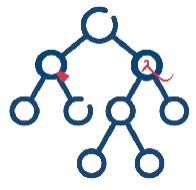
\includegraphics[height=1.0cm]{msca_logo.png}}%
    \end{center}

    \vspace{0.6cm}

    % Main title with Q logos on sides (with clickable links)
    \begin{center}
        \begin{minipage}{0.1\textwidth}
            \centering
            \href{https://quantlet.com}{
\includegraphics[height=1.1cm]{ql_logo.png}}
        \end{minipage}%
        \begin{minipage}{0.78\textwidth}
            \centering
            {\LARGE\bfseries\usebeamercolor[fg]{title}\inserttitle}

            \vspace{0.3cm}

            {\usebeamerfont{subtitle}\usebeamercolor[fg]{title}\insertsubtitle}
        \end{minipage}%
        \begin{minipage}{0.1\textwidth}
            \centering
            \href{https://quantinar.com}{
\includegraphics[height=1.1cm]{qr_logo.png}}
        \end{minipage}
    \end{center}

    \vspace{0.6cm}

    % Authors (left aligned)
    \hspace{0.5cm}{\usebeamerfont{author}\insertauthor}

    \vspace{0.3cm}

    % Institute/Affiliations (left aligned)
    \hspace{0.5cm}\begin{minipage}[t]{0.9\textwidth}
        \raggedright\small\insertinstitute
    \end{minipage}
}

%=============================================================================
% THEOREM ENVIRONMENTS
%=============================================================================
\theoremstyle{definition}
\setbeamertemplate{theorems}[numbered]
\ifdefined\atslang
\newtheorem{defn}{Definiție}
\newtheorem{thm}{Teoremă}
\newtheorem{prop}{Propoziție}
\newtheorem{rmk}{Observație}
\else
\newtheorem{defn}{Definition}
\newtheorem{thm}{Theorem}
\newtheorem{prop}{Proposition}
\newtheorem{rmk}{Remark}
\fi

%=============================================================================
% CENTRED MINIPAGE (no extra vertical space)
%=============================================================================
\newenvironment{cminipage}[1]{%
    \par\noindent\hfill\begin{minipage}{#1}\ignorespaces
}{%
    \end{minipage}\hfill\null\par
}

%=============================================================================
% CUSTOM COMMANDS
%=============================================================================
\newcommand{\E}{\mathbb{E}}
\newcommand{\Var}{\text{Var}}
\newcommand{\Cov}{\text{Cov}}
\newcommand{\Corr}{\text{Corr}}
\newcommand{\R}{\mathbb{R}}
\newcommand{\N}{\mathbb{N}}
\newcommand{\Z}{\mathbb{Z}}
\newcommand{\B}{\mathbf{B}}
\newcommand{\imark}{\textcolor{MainBlue}{\textbullet}}
\newcommand{\RMSE}{\text{RMSE}}
\newcommand{\MAE}{\text{MAE}}
\newcommand{\MAPE}{\text{MAPE}}

% Boldface vector/matrix commands (VAR, VECM, state space)
\newcommand{\bY}{\mathbf{Y}}
\newcommand{\bX}{\mathbf{X}}
\newcommand{\bA}{\mathbf{A}}
\newcommand{\bB}{\mathbf{B}}
\newcommand{\bepsilon}{\boldsymbol{\varepsilon}}
\newcommand{\bSigma}{\boldsymbol{\Sigma}}
\newcommand{\bPhi}{\boldsymbol{\Phi}}
\newcommand{\bGamma}{\boldsymbol{\Gamma}}
\newcommand{\bPi}{\boldsymbol{\Pi}}
\newcommand{\bc}{\mathbf{c}}
\newcommand{\balpha}{\boldsymbol{\alpha}}
\newcommand{\bbeta}{\boldsymbol{\beta}}
\newcommand{\bvarepsilon}{\boldsymbol{\varepsilon}}

% Seminar marks
\newcommand{\correct}{\textcolor{Forest}{\checkmark}}
\newcommand{\incorrect}{\textcolor{Crimson}{\texttimes}}
 se definește
%   \newcommand{\coursename}{Advanced Time Series Analysis and Forecasting}          (EN)
%   \newcommand{\coursename}{Analiza avansată a seriilor de timp și previziune}       (RO)  și  \def\atslang{ro}
% Fișierele .tex se află în EN/Courses, EN/Seminars, RO/Cursuri, RO/Seminarii (două niveluri sub rădăcină).
% Deck-urile sînt generate de latex/build_chapterN.py / build_seminarN.py (vezi latex/ats_build.py).

\documentclass[9pt, aspectratio=169, t]{beamer}
\providecommand{\coursename}{Advanced Time Series Analysis and Forecasting}

% Ensure content fits on slides
\setbeamersize{text margin left=8mm, text margin right=8mm}
% Smaller institute font (title page)
\setbeamerfont{institute}{size=\footnotesize}

%=============================================================================
% THEME AND STYLE CONFIGURATION
%=============================================================================
\usetheme{default}
% Using default theme for clean header/footer control

% Color Palette (matching Redispatch PDF)
\definecolor{MainBlue}{RGB}{26, 58, 110}
\definecolor{AccentBlue}{RGB}{26, 58, 110}
\definecolor{IDAred}{RGB}{205, 0, 0}
\definecolor{DarkGray}{RGB}{51, 51, 51}
\definecolor{MediumGray}{RGB}{128, 128, 128}
\definecolor{LightGray}{RGB}{248, 248, 248}
\definecolor{VeryLightGray}{RGB}{235, 235, 235}
\definecolor{KeynoteGray}{RGB}{218, 218, 218}
\definecolor{SectionGray}{RGB}{120, 120, 120}
\definecolor{FooterGray}{RGB}{100, 100, 100}
\definecolor{Crimson}{RGB}{220, 53, 69}
\definecolor{Forest}{RGB}{46, 125, 50}
\definecolor{Amber}{RGB}{181, 133, 63}
\definecolor{Orange}{RGB}{230, 126, 34}
\definecolor{Purple}{RGB}{142, 68, 173}

% Gradient background (exact Keynote 315° gradient: white to RGB 218,218,218)
\setbeamertemplate{background}{%
    \begin{tikzpicture}[remember picture, overlay]
        \shade[shading=axis, shading angle=315,
        top color=white, bottom color=KeynoteGray]
        (current page.south west) rectangle (current page.north east);
    \end{tikzpicture}%
}
% Fallback solid color for compatibility
\setbeamercolor{background canvas}{bg=}

\setbeamercolor{palette primary}{bg=MainBlue, fg=white}
\setbeamercolor{palette secondary}{bg=MainBlue!85, fg=white}
\setbeamercolor{palette tertiary}{bg=MainBlue!70, fg=white}
\setbeamercolor{structure}{fg=MainBlue}
\setbeamercolor{title}{fg=IDAred}
\setbeamercolor{frametitle}{fg=IDAred, bg=}
\setbeamercolor{block title}{bg=MainBlue, fg=white}
\setbeamercolor{block body}{bg=VeryLightGray, fg=DarkGray}
\setbeamercolor{block title alerted}{bg=Crimson, fg=white}
\setbeamercolor{block body alerted}{bg=Crimson!8, fg=DarkGray}
\setbeamercolor{block title example}{bg=Forest, fg=white}
\setbeamercolor{block body example}{bg=Forest!8, fg=DarkGray}
\setbeamercolor{item}{fg=MainBlue}

% Footer colors (override Madrid theme blue)
\setbeamercolor{author in head/foot}{fg=FooterGray, bg=}
\setbeamercolor{title in head/foot}{fg=FooterGray, bg=}
\setbeamercolor{date in head/foot}{fg=FooterGray, bg=}
\setbeamercolor{section in head/foot}{fg=FooterGray, bg=}
\setbeamercolor{subsection in head/foot}{fg=FooterGray, bg=}

% Bullet styles (apply everywhere including blocks)
\setbeamertemplate{itemize item}{\color{MainBlue}$\boxdot$}
\setbeamertemplate{itemize subitem}{\color{MainBlue}$\blacktriangleright$}
\setbeamertemplate{itemize subsubitem}{\color{MainBlue}\tiny$\bullet$}
\setbeamertemplate{itemize/enumerate body begin}{\normalsize}
\setbeamertemplate{itemize/enumerate subbody begin}{\normalsize}

% Item spacing - compact style
\setlength{\leftmargini}{10pt}       % Level 1: minimal indent
\setlength{\leftmarginii}{10pt}      % Level 2: minimal additional indent
% Compact list spacing (zero extra space before/after lists in blocks)
\makeatletter
\def\@listi{\leftmargin\leftmargini \topsep 0pt \parsep 0pt \itemsep 0pt}
\def\@listii{\leftmargin\leftmarginii \topsep 0pt \parsep 0pt \itemsep 0pt}
\makeatother

\setbeamertemplate{navigation symbols}{}

%=============================================================================
% CUSTOM HEADLINE
%=============================================================================
\setbeamertemplate{headline}{%
    \vskip10pt%
    \hbox to \paperwidth{%
        \hskip0.5cm%
        {\small\color{FooterGray}\renewcommand{\hyperlink}[2]{##2}\insertsectionhead}%
        \hfill%
        \textcolor{FooterGray}{\small\insertframenumber}%
        \hskip0.5cm%
    }%
    \vskip4pt%
    {\color{FooterGray}\hrule height 0.4pt}%
}

%=============================================================================
% CUSTOM FOOTER
%=============================================================================
\usepackage{fontawesome5}

\setbeamertemplate{footline}{%
    {\color{FooterGray}\hrule height 0.4pt}%
    \vskip4pt%
    \hbox to \paperwidth{%
        \hskip0.5cm%
        \textcolor{FooterGray}{\small\coursename}%
        \hfill%
        \raisebox{-0.1em}{%
            \begin{tikzpicture}[x=0.08em, y=0.08em, line width=0.4pt]
                \draw[FooterGray] (0,3) -- (1,4) -- (2,3.5) -- (3,5) -- (4,4) -- (5,6) -- (6,5.5) -- (7,4) -- (8,5) -- (9,7) -- (10,6) -- (11,5) -- (12,6.5) -- (13,8) -- (14,7) -- (15,6) -- (16,7.5) -- (17,9) -- (18,8) -- (19,7) -- (20,8.5) -- (21,10) -- (22,9) -- (23,8) -- (24,9.5);
            \end{tikzpicture}%
        }%
        \hskip0.5cm%
    }%
    \vskip6pt%
}

%=============================================================================
% PACKAGES
%=============================================================================
\usepackage[utf8]{inputenc}
\DeclareUnicodeCharacter{03B1}{\ensuremath{\alpha}}
\usepackage[T1]{fontenc}
\usepackage{amsmath, amssymb, amsthm}
\usepackage{mathtools}
\usepackage{bm}
\usepackage{tikz}
\usetikzlibrary{arrows.meta, positioning, shapes, calc, decorations.pathreplacing, shadings}
\usepackage{booktabs}
\usepackage{multirow}
\usepackage{array}
\usepackage{graphicx}
\usepackage{animate}
\usepackage{hyperref}
\usepackage{colortbl}
\usepackage{listings}
\lstset{language=Python, basicstyle=\ttfamily\scriptsize, keywordstyle=\color{MainBlue}\bfseries,
  commentstyle=\color{Forest}, stringstyle=\color{Crimson}, breaklines=true,
  frame=none, backgroundcolor=\color{VeryLightGray}, xleftmargin=2mm}
\hypersetup{colorlinks=true, linkcolor=MainBlue, urlcolor=MainBlue}
\graphicspath{{../../logos/}{../../charts/}{../../photos/}}
\usepackage{xcolor}
\hfuzz=2pt  % Suppress tiny overfull warnings (<2pt)
\vfuzz=2pt  % Suppress tiny vertical overfull warnings (<2pt)

%=============================================================================
% QUANTLET COMMANDS
%   \quantlet{<displayed name>}{<url>}       (generic)
%   \atsquantlet{Ch_05}{ATS_ch5_garch}       -> https://github.com/danpele/Advanced-Time-Series/tree/main/Quantlets/Ch_05/ATS_ch5_garch
%   \qlurl{<folder>} is defined per chapter by the generator (Quantlets/Ch_NN/<folder>)
%=============================================================================
\newcommand{\atsrepo}{https://github.com/danpele/Advanced-Time-Series}
\newcommand{\atsqlbase}{https://github.com/danpele/Advanced-Time-Series/tree/main/Quantlets}
\newcommand{\quantlet}[2]{%
    \hfill\href{#2}{%
        \raisebox{-0.15em}{
\includegraphics[height=0.7em]{ql_logo.png}}%
        \textcolor{MainBlue}{\tiny\ #1}%
    }%
}
\newcommand{\atsquantlet}[2]{\quantlet{\detokenize{#2}}{\atsqlbase/#1/#2}}

%=============================================================================
% NOTEBOOKS (Google Colab)
%   \colaburl{notebooks/EN/chapter5_seminar_notebook.ipynb} -> the Colab link of a file in the ATS repo
%   \nb: the chapter notebook (each seminar deck redefines it with \renewcommand)
%=============================================================================
\newcommand{\colaburl}[1]{https://colab.research.google.com/github/danpele/Advanced-Time-Series/blob/main/#1}
\newcommand{\nb}{https://colab.research.google.com/github/danpele/Advanced-Time-Series/tree/main/notebooks/EN}
\newcommand{\nbname}{notebooks/EN}

%=============================================================================
% SLIDE HELPERS (used by the generators; the same as in MFM)
%=============================================================================
% local font size for list bodies (the preamble forces \normalsize)
\newcommand{\itemsize}[1]{\setbeamertemplate{itemize/enumerate body begin}{#1}\setbeamertemplate{itemize/enumerate subbody begin}{#1}}
\newcommand{\intitle}[1]{{\hypersetup{urlcolor=white}#1}}   % white links inside coloured title bars
\newcommand{\imgcap}[1]{{\scriptsize #1}\\[0.5mm]}          % caption under a photo
\newcommand{\imgcredit}[2]{{\tiny\color{FooterGray}\href{#1}{#2}}}   % image credit: source URL, author/licence
\newcommand{\aiprompt}[1]{{\ttfamily\color{MainBlue}#1}}     % a prompt to an AI assistant

%=============================================================================
% SEMINARS: student version by default; the instructor wrapper *_solutions.tex sets \solutionstrue
%=============================================================================
\makeatletter\@ifundefined{ifsolutions}{\expandafter\newif\csname ifsolutions\endcsname}{}\makeatother
\newcommand{\solonly}[1]{\ifsolutions #1\fi}
\newcommand{\propsub}{\ifsolutions\else\framesubtitle{\ifdefined\atslang Rezolvarea se discută la seminar\else Solution discussed in class\fi}\fi}

%=============================================================================
% APPENDIX AND CHAPTER LINKS (latex/appendix_links.py writes the calls; it also re-declares these
% macros before \begin{document}, so the decks compile with or without this preamble block)
%=============================================================================
\providecommand{\atsapplink}[3]{\hypertarget{#2}{}\hyperlink{#1}{\beamergotobutton{#3}}}
\providecommand{\atsappback}[2]{\begin{tikzpicture}[remember picture,overlay]\node[anchor=south east] at ([xshift=-3mm,yshift=7mm]current page.south east){\hyperlink{#1}{\beamerreturnbutton{#2}}};\end{tikzpicture}}
\providecommand{\atschlink}[2]{\href{#1}{#2}}
\providecommand{\atschlinkt}[2]{\href{#1}{\usebeamercolor[fg]{frametitle}#2}}

%=============================================================================
% QUANTINAR COMMAND: link către un curs Quantinar (subiecte avansate)
%=============================================================================
\newcommand{\quantinar}[2]{%
    \href{#2}{%
        \raisebox{-0.15em}{
\includegraphics[height=0.8em]{qr_logo.png}}%
        \textcolor{MainBlue}{\scriptsize\ #1}%
    }%
}

%=============================================================================
% CUSTOM TITLE PAGE
%=============================================================================
\defbeamertemplate*{title page}{hybrid}[1][]
{
    \vspace{0.2cm}
    % Logos row - top header (with clickable links)
    \begin{center}
        \href{https://www.ase.ro}{
\includegraphics[height=1.0cm]{ase_logo.png}}\hspace{0.3cm}%
        \href{https://theida.net}{
\includegraphics[height=1.0cm]{ida_logo.png}}\hspace{0.3cm}%
        \href{https://blockchain-research-center.com}{
\includegraphics[height=1.0cm]{brc_logo.png}}\hspace{0.3cm}%
        \href{https://www.ai4efin.ase.ro}{
\includegraphics[height=1.0cm]{ai4efin_logo.png}}\hspace{0.3cm}%
        \href{https://ipe.ro/new}{
\includegraphics[height=1.0cm]{acad_logo.png}}\hspace{0.3cm}%
        \href{https://www.digital-finance-msca.com}{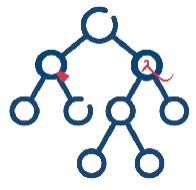
\includegraphics[height=1.0cm]{msca_logo.png}}%
    \end{center}

    \vspace{0.6cm}

    % Main title with Q logos on sides (with clickable links)
    \begin{center}
        \begin{minipage}{0.1\textwidth}
            \centering
            \href{https://quantlet.com}{
\includegraphics[height=1.1cm]{ql_logo.png}}
        \end{minipage}%
        \begin{minipage}{0.78\textwidth}
            \centering
            {\LARGE\bfseries\usebeamercolor[fg]{title}\inserttitle}

            \vspace{0.3cm}

            {\usebeamerfont{subtitle}\usebeamercolor[fg]{title}\insertsubtitle}
        \end{minipage}%
        \begin{minipage}{0.1\textwidth}
            \centering
            \href{https://quantinar.com}{
\includegraphics[height=1.1cm]{qr_logo.png}}
        \end{minipage}
    \end{center}

    \vspace{0.6cm}

    % Authors (left aligned)
    \hspace{0.5cm}{\usebeamerfont{author}\insertauthor}

    \vspace{0.3cm}

    % Institute/Affiliations (left aligned)
    \hspace{0.5cm}\begin{minipage}[t]{0.9\textwidth}
        \raggedright\small\insertinstitute
    \end{minipage}
}

%=============================================================================
% THEOREM ENVIRONMENTS
%=============================================================================
\theoremstyle{definition}
\setbeamertemplate{theorems}[numbered]
\ifdefined\atslang
\newtheorem{defn}{Definiție}
\newtheorem{thm}{Teoremă}
\newtheorem{prop}{Propoziție}
\newtheorem{rmk}{Observație}
\else
\newtheorem{defn}{Definition}
\newtheorem{thm}{Theorem}
\newtheorem{prop}{Proposition}
\newtheorem{rmk}{Remark}
\fi

%=============================================================================
% CENTRED MINIPAGE (no extra vertical space)
%=============================================================================
\newenvironment{cminipage}[1]{%
    \par\noindent\hfill\begin{minipage}{#1}\ignorespaces
}{%
    \end{minipage}\hfill\null\par
}

%=============================================================================
% CUSTOM COMMANDS
%=============================================================================
\newcommand{\E}{\mathbb{E}}
\newcommand{\Var}{\text{Var}}
\newcommand{\Cov}{\text{Cov}}
\newcommand{\Corr}{\text{Corr}}
\newcommand{\R}{\mathbb{R}}
\newcommand{\N}{\mathbb{N}}
\newcommand{\Z}{\mathbb{Z}}
\newcommand{\B}{\mathbf{B}}
\newcommand{\imark}{\textcolor{MainBlue}{\textbullet}}
\newcommand{\RMSE}{\text{RMSE}}
\newcommand{\MAE}{\text{MAE}}
\newcommand{\MAPE}{\text{MAPE}}

% Boldface vector/matrix commands (VAR, VECM, state space)
\newcommand{\bY}{\mathbf{Y}}
\newcommand{\bX}{\mathbf{X}}
\newcommand{\bA}{\mathbf{A}}
\newcommand{\bB}{\mathbf{B}}
\newcommand{\bepsilon}{\boldsymbol{\varepsilon}}
\newcommand{\bSigma}{\boldsymbol{\Sigma}}
\newcommand{\bPhi}{\boldsymbol{\Phi}}
\newcommand{\bGamma}{\boldsymbol{\Gamma}}
\newcommand{\bPi}{\boldsymbol{\Pi}}
\newcommand{\bc}{\mathbf{c}}
\newcommand{\balpha}{\boldsymbol{\alpha}}
\newcommand{\bbeta}{\boldsymbol{\beta}}
\newcommand{\bvarepsilon}{\boldsymbol{\varepsilon}}

% Seminar marks
\newcommand{\correct}{\textcolor{Forest}{\checkmark}}
\newcommand{\incorrect}{\textcolor{Crimson}{\texttimes}}
 se definește
%   \newcommand{\coursename}{Advanced Time Series Analysis and Forecasting}          (EN)
%   \newcommand{\coursename}{Analiza avansată a seriilor de timp și previziune}       (RO)  și  \def\atslang{ro}
% Fișierele .tex se află în EN/Courses, EN/Seminars, RO/Cursuri, RO/Seminarii (două niveluri sub rădăcină).
% Deck-urile sînt generate de latex/build_chapterN.py / build_seminarN.py (vezi latex/ats_build.py).

\documentclass[9pt, aspectratio=169, t]{beamer}
\providecommand{\coursename}{Advanced Time Series Analysis and Forecasting}

% Ensure content fits on slides
\setbeamersize{text margin left=8mm, text margin right=8mm}
% Smaller institute font (title page)
\setbeamerfont{institute}{size=\footnotesize}

%=============================================================================
% THEME AND STYLE CONFIGURATION
%=============================================================================
\usetheme{default}
% Using default theme for clean header/footer control

% Color Palette (matching Redispatch PDF)
\definecolor{MainBlue}{RGB}{26, 58, 110}
\definecolor{AccentBlue}{RGB}{26, 58, 110}
\definecolor{IDAred}{RGB}{205, 0, 0}
\definecolor{DarkGray}{RGB}{51, 51, 51}
\definecolor{MediumGray}{RGB}{128, 128, 128}
\definecolor{LightGray}{RGB}{248, 248, 248}
\definecolor{VeryLightGray}{RGB}{235, 235, 235}
\definecolor{KeynoteGray}{RGB}{218, 218, 218}
\definecolor{SectionGray}{RGB}{120, 120, 120}
\definecolor{FooterGray}{RGB}{100, 100, 100}
\definecolor{Crimson}{RGB}{220, 53, 69}
\definecolor{Forest}{RGB}{46, 125, 50}
\definecolor{Amber}{RGB}{181, 133, 63}
\definecolor{Orange}{RGB}{230, 126, 34}
\definecolor{Purple}{RGB}{142, 68, 173}

% Gradient background (exact Keynote 315° gradient: white to RGB 218,218,218)
\setbeamertemplate{background}{%
    \begin{tikzpicture}[remember picture, overlay]
        \shade[shading=axis, shading angle=315,
        top color=white, bottom color=KeynoteGray]
        (current page.south west) rectangle (current page.north east);
    \end{tikzpicture}%
}
% Fallback solid color for compatibility
\setbeamercolor{background canvas}{bg=}

\setbeamercolor{palette primary}{bg=MainBlue, fg=white}
\setbeamercolor{palette secondary}{bg=MainBlue!85, fg=white}
\setbeamercolor{palette tertiary}{bg=MainBlue!70, fg=white}
\setbeamercolor{structure}{fg=MainBlue}
\setbeamercolor{title}{fg=IDAred}
\setbeamercolor{frametitle}{fg=IDAred, bg=}
\setbeamercolor{block title}{bg=MainBlue, fg=white}
\setbeamercolor{block body}{bg=VeryLightGray, fg=DarkGray}
\setbeamercolor{block title alerted}{bg=Crimson, fg=white}
\setbeamercolor{block body alerted}{bg=Crimson!8, fg=DarkGray}
\setbeamercolor{block title example}{bg=Forest, fg=white}
\setbeamercolor{block body example}{bg=Forest!8, fg=DarkGray}
\setbeamercolor{item}{fg=MainBlue}

% Footer colors (override Madrid theme blue)
\setbeamercolor{author in head/foot}{fg=FooterGray, bg=}
\setbeamercolor{title in head/foot}{fg=FooterGray, bg=}
\setbeamercolor{date in head/foot}{fg=FooterGray, bg=}
\setbeamercolor{section in head/foot}{fg=FooterGray, bg=}
\setbeamercolor{subsection in head/foot}{fg=FooterGray, bg=}

% Bullet styles (apply everywhere including blocks)
\setbeamertemplate{itemize item}{\color{MainBlue}$\boxdot$}
\setbeamertemplate{itemize subitem}{\color{MainBlue}$\blacktriangleright$}
\setbeamertemplate{itemize subsubitem}{\color{MainBlue}\tiny$\bullet$}
\setbeamertemplate{itemize/enumerate body begin}{\normalsize}
\setbeamertemplate{itemize/enumerate subbody begin}{\normalsize}

% Item spacing - compact style
\setlength{\leftmargini}{10pt}       % Level 1: minimal indent
\setlength{\leftmarginii}{10pt}      % Level 2: minimal additional indent
% Compact list spacing (zero extra space before/after lists in blocks)
\makeatletter
\def\@listi{\leftmargin\leftmargini \topsep 0pt \parsep 0pt \itemsep 0pt}
\def\@listii{\leftmargin\leftmarginii \topsep 0pt \parsep 0pt \itemsep 0pt}
\makeatother

\setbeamertemplate{navigation symbols}{}

%=============================================================================
% CUSTOM HEADLINE
%=============================================================================
\setbeamertemplate{headline}{%
    \vskip10pt%
    \hbox to \paperwidth{%
        \hskip0.5cm%
        {\small\color{FooterGray}\renewcommand{\hyperlink}[2]{##2}\insertsectionhead}%
        \hfill%
        \textcolor{FooterGray}{\small\insertframenumber}%
        \hskip0.5cm%
    }%
    \vskip4pt%
    {\color{FooterGray}\hrule height 0.4pt}%
}

%=============================================================================
% CUSTOM FOOTER
%=============================================================================
\usepackage{fontawesome5}

\setbeamertemplate{footline}{%
    {\color{FooterGray}\hrule height 0.4pt}%
    \vskip4pt%
    \hbox to \paperwidth{%
        \hskip0.5cm%
        \textcolor{FooterGray}{\small\coursename}%
        \hfill%
        \raisebox{-0.1em}{%
            \begin{tikzpicture}[x=0.08em, y=0.08em, line width=0.4pt]
                \draw[FooterGray] (0,3) -- (1,4) -- (2,3.5) -- (3,5) -- (4,4) -- (5,6) -- (6,5.5) -- (7,4) -- (8,5) -- (9,7) -- (10,6) -- (11,5) -- (12,6.5) -- (13,8) -- (14,7) -- (15,6) -- (16,7.5) -- (17,9) -- (18,8) -- (19,7) -- (20,8.5) -- (21,10) -- (22,9) -- (23,8) -- (24,9.5);
            \end{tikzpicture}%
        }%
        \hskip0.5cm%
    }%
    \vskip6pt%
}

%=============================================================================
% PACKAGES
%=============================================================================
\usepackage[utf8]{inputenc}
\DeclareUnicodeCharacter{03B1}{\ensuremath{\alpha}}
\usepackage[T1]{fontenc}
\usepackage{amsmath, amssymb, amsthm}
\usepackage{mathtools}
\usepackage{bm}
\usepackage{tikz}
\usetikzlibrary{arrows.meta, positioning, shapes, calc, decorations.pathreplacing, shadings}
\usepackage{booktabs}
\usepackage{multirow}
\usepackage{array}
\usepackage{graphicx}
\usepackage{animate}
\usepackage{hyperref}
\usepackage{colortbl}
\usepackage{listings}
\lstset{language=Python, basicstyle=\ttfamily\scriptsize, keywordstyle=\color{MainBlue}\bfseries,
  commentstyle=\color{Forest}, stringstyle=\color{Crimson}, breaklines=true,
  frame=none, backgroundcolor=\color{VeryLightGray}, xleftmargin=2mm}
\hypersetup{colorlinks=true, linkcolor=MainBlue, urlcolor=MainBlue}
\graphicspath{{../../logos/}{../../charts/}{../../photos/}}
\usepackage{xcolor}
\hfuzz=2pt  % Suppress tiny overfull warnings (<2pt)
\vfuzz=2pt  % Suppress tiny vertical overfull warnings (<2pt)

%=============================================================================
% QUANTLET COMMANDS
%   \quantlet{<displayed name>}{<url>}       (generic)
%   \atsquantlet{Ch_05}{ATS_ch5_garch}       -> https://github.com/danpele/Advanced-Time-Series/tree/main/Quantlets/Ch_05/ATS_ch5_garch
%   \qlurl{<folder>} is defined per chapter by the generator (Quantlets/Ch_NN/<folder>)
%=============================================================================
\newcommand{\atsrepo}{https://github.com/danpele/Advanced-Time-Series}
\newcommand{\atsqlbase}{https://github.com/danpele/Advanced-Time-Series/tree/main/Quantlets}
\newcommand{\quantlet}[2]{%
    \hfill\href{#2}{%
        \raisebox{-0.15em}{
\includegraphics[height=0.7em]{ql_logo.png}}%
        \textcolor{MainBlue}{\tiny\ #1}%
    }%
}
\newcommand{\atsquantlet}[2]{\quantlet{\detokenize{#2}}{\atsqlbase/#1/#2}}

%=============================================================================
% NOTEBOOKS (Google Colab)
%   \colaburl{notebooks/EN/chapter5_seminar_notebook.ipynb} -> the Colab link of a file in the ATS repo
%   \nb: the chapter notebook (each seminar deck redefines it with \renewcommand)
%=============================================================================
\newcommand{\colaburl}[1]{https://colab.research.google.com/github/danpele/Advanced-Time-Series/blob/main/#1}
\newcommand{\nb}{https://colab.research.google.com/github/danpele/Advanced-Time-Series/tree/main/notebooks/EN}
\newcommand{\nbname}{notebooks/EN}

%=============================================================================
% SLIDE HELPERS (used by the generators; the same as in MFM)
%=============================================================================
% local font size for list bodies (the preamble forces \normalsize)
\newcommand{\itemsize}[1]{\setbeamertemplate{itemize/enumerate body begin}{#1}\setbeamertemplate{itemize/enumerate subbody begin}{#1}}
\newcommand{\intitle}[1]{{\hypersetup{urlcolor=white}#1}}   % white links inside coloured title bars
\newcommand{\imgcap}[1]{{\scriptsize #1}\\[0.5mm]}          % caption under a photo
\newcommand{\imgcredit}[2]{{\tiny\color{FooterGray}\href{#1}{#2}}}   % image credit: source URL, author/licence
\newcommand{\aiprompt}[1]{{\ttfamily\color{MainBlue}#1}}     % a prompt to an AI assistant

%=============================================================================
% SEMINARS: student version by default; the instructor wrapper *_solutions.tex sets \solutionstrue
%=============================================================================
\makeatletter\@ifundefined{ifsolutions}{\expandafter\newif\csname ifsolutions\endcsname}{}\makeatother
\newcommand{\solonly}[1]{\ifsolutions #1\fi}
\newcommand{\propsub}{\ifsolutions\else\framesubtitle{\ifdefined\atslang Rezolvarea se discută la seminar\else Solution discussed in class\fi}\fi}

%=============================================================================
% APPENDIX AND CHAPTER LINKS (latex/appendix_links.py writes the calls; it also re-declares these
% macros before \begin{document}, so the decks compile with or without this preamble block)
%=============================================================================
\providecommand{\atsapplink}[3]{\hypertarget{#2}{}\hyperlink{#1}{\beamergotobutton{#3}}}
\providecommand{\atsappback}[2]{\begin{tikzpicture}[remember picture,overlay]\node[anchor=south east] at ([xshift=-3mm,yshift=7mm]current page.south east){\hyperlink{#1}{\beamerreturnbutton{#2}}};\end{tikzpicture}}
\providecommand{\atschlink}[2]{\href{#1}{#2}}
\providecommand{\atschlinkt}[2]{\href{#1}{\usebeamercolor[fg]{frametitle}#2}}

%=============================================================================
% QUANTINAR COMMAND: link către un curs Quantinar (subiecte avansate)
%=============================================================================
\newcommand{\quantinar}[2]{%
    \href{#2}{%
        \raisebox{-0.15em}{
\includegraphics[height=0.8em]{qr_logo.png}}%
        \textcolor{MainBlue}{\scriptsize\ #1}%
    }%
}

%=============================================================================
% CUSTOM TITLE PAGE
%=============================================================================
\defbeamertemplate*{title page}{hybrid}[1][]
{
    \vspace{0.2cm}
    % Logos row - top header (with clickable links)
    \begin{center}
        \href{https://www.ase.ro}{
\includegraphics[height=1.0cm]{ase_logo.png}}\hspace{0.3cm}%
        \href{https://theida.net}{
\includegraphics[height=1.0cm]{ida_logo.png}}\hspace{0.3cm}%
        \href{https://blockchain-research-center.com}{
\includegraphics[height=1.0cm]{brc_logo.png}}\hspace{0.3cm}%
        \href{https://www.ai4efin.ase.ro}{
\includegraphics[height=1.0cm]{ai4efin_logo.png}}\hspace{0.3cm}%
        \href{https://ipe.ro/new}{
\includegraphics[height=1.0cm]{acad_logo.png}}\hspace{0.3cm}%
        \href{https://www.digital-finance-msca.com}{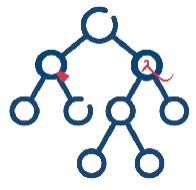
\includegraphics[height=1.0cm]{msca_logo.png}}%
    \end{center}

    \vspace{0.6cm}

    % Main title with Q logos on sides (with clickable links)
    \begin{center}
        \begin{minipage}{0.1\textwidth}
            \centering
            \href{https://quantlet.com}{
\includegraphics[height=1.1cm]{ql_logo.png}}
        \end{minipage}%
        \begin{minipage}{0.78\textwidth}
            \centering
            {\LARGE\bfseries\usebeamercolor[fg]{title}\inserttitle}

            \vspace{0.3cm}

            {\usebeamerfont{subtitle}\usebeamercolor[fg]{title}\insertsubtitle}
        \end{minipage}%
        \begin{minipage}{0.1\textwidth}
            \centering
            \href{https://quantinar.com}{
\includegraphics[height=1.1cm]{qr_logo.png}}
        \end{minipage}
    \end{center}

    \vspace{0.6cm}

    % Authors (left aligned)
    \hspace{0.5cm}{\usebeamerfont{author}\insertauthor}

    \vspace{0.3cm}

    % Institute/Affiliations (left aligned)
    \hspace{0.5cm}\begin{minipage}[t]{0.9\textwidth}
        \raggedright\small\insertinstitute
    \end{minipage}
}

%=============================================================================
% THEOREM ENVIRONMENTS
%=============================================================================
\theoremstyle{definition}
\setbeamertemplate{theorems}[numbered]
\ifdefined\atslang
\newtheorem{defn}{Definiție}
\newtheorem{thm}{Teoremă}
\newtheorem{prop}{Propoziție}
\newtheorem{rmk}{Observație}
\else
\newtheorem{defn}{Definition}
\newtheorem{thm}{Theorem}
\newtheorem{prop}{Proposition}
\newtheorem{rmk}{Remark}
\fi

%=============================================================================
% CENTRED MINIPAGE (no extra vertical space)
%=============================================================================
\newenvironment{cminipage}[1]{%
    \par\noindent\hfill\begin{minipage}{#1}\ignorespaces
}{%
    \end{minipage}\hfill\null\par
}

%=============================================================================
% CUSTOM COMMANDS
%=============================================================================
\newcommand{\E}{\mathbb{E}}
\newcommand{\Var}{\text{Var}}
\newcommand{\Cov}{\text{Cov}}
\newcommand{\Corr}{\text{Corr}}
\newcommand{\R}{\mathbb{R}}
\newcommand{\N}{\mathbb{N}}
\newcommand{\Z}{\mathbb{Z}}
\newcommand{\B}{\mathbf{B}}
\newcommand{\imark}{\textcolor{MainBlue}{\textbullet}}
\newcommand{\RMSE}{\text{RMSE}}
\newcommand{\MAE}{\text{MAE}}
\newcommand{\MAPE}{\text{MAPE}}

% Boldface vector/matrix commands (VAR, VECM, state space)
\newcommand{\bY}{\mathbf{Y}}
\newcommand{\bX}{\mathbf{X}}
\newcommand{\bA}{\mathbf{A}}
\newcommand{\bB}{\mathbf{B}}
\newcommand{\bepsilon}{\boldsymbol{\varepsilon}}
\newcommand{\bSigma}{\boldsymbol{\Sigma}}
\newcommand{\bPhi}{\boldsymbol{\Phi}}
\newcommand{\bGamma}{\boldsymbol{\Gamma}}
\newcommand{\bPi}{\boldsymbol{\Pi}}
\newcommand{\bc}{\mathbf{c}}
\newcommand{\balpha}{\boldsymbol{\alpha}}
\newcommand{\bbeta}{\boldsymbol{\beta}}
\newcommand{\bvarepsilon}{\boldsymbol{\varepsilon}}

% Seminar marks
\newcommand{\correct}{\textcolor{Forest}{\checkmark}}
\newcommand{\incorrect}{\textcolor{Crimson}{\texttimes}}


\newcommand{\qlurl}[1]{https://github.com/danpele/Advanced-Time-Series/tree/main/Quantlets/Ch_11/#1}

% Clickable citations (DOIs verified via Crossref)
\newcommand{\refACS}{\href{https://doi.org/10.1111/joes.12012}{Aguiar-Conraria and Soares (2014)}}
\newcommand{\refAAS}{\href{https://doi.org/10.1016/j.physa.2008.01.063}{Aguiar-Conraria, Azevedo and Soares (2008)}}
\newcommand{\refAnd}{\href{https://doi.org/10.2307/2938229}{Andrews (1991)}}
\newcommand{\refBK}{\href{https://doi.org/10.1162/003465399558454}{Baxter and King (1999)}}
\newcommand{\refBC}{\href{https://doi.org/10.1016/j.jeconom.2005.02.004}{Breitung and Candelon (2006)}}
\newcommand{\refBD}{\href{https://doi.org/10.1007/978-1-4419-0320-4}{Brockwell and Davis (1991)}}
\newcommand{\refCF}{\href{https://doi.org/10.1111/1468-2354.t01-1-00076}{Christiano and Fitzgerald (2003)}}
\newcommand{\refCN}{\href{https://doi.org/10.1016/0165-1889(93)00781-X}{Cogley and Nason (1995)}}
\newcommand{\refCFR}{\href{https://doi.org/10.1162/00346530151143770}{Croux, Forni and Reichlin (2001)}}
\newcommand{\refCro}{\href{https://doi.org/10.1111/j.1467-6419.2006.00502.x}{Crowley (2007)}}
\newcommand{\refDah}{\href{https://doi.org/10.1214/aos/1034276620}{Dahlhaus (1997)}}
\newcommand{\refDau}{\href{https://doi.org/10.1002/cpa.3160410705}{Daubechies (1988)}}
\newcommand{\refFK}{\href{https://doi.org/10.1016/j.jce.2006.06.007}{Fidrmuc and Korhonen (2006)}}
\newcommand{\refFR}{\href{https://doi.org/10.1111/0022-1082.00494}{Forbes and Rigobon (2002)}}
\newcommand{\refGSW}{\href{https://doi.org/10.1016/j.jimonfin.2004.10.003}{Gençay, Selçuk and Whitcher (2005)}}
\newcommand{\refGSWb}{\href{https://doi.org/10.1016/B978-012279670-8.50010-0}{Gençay, Selçuk and Whitcher (2002)}}
\newcommand{\refGew}{\href{https://doi.org/10.1080/01621459.1982.10477803}{Geweke (1982)}}
\newcommand{\refGra}{\href{https://doi.org/10.2307/1909859}{Granger (1966)}}
\newcommand{\refGMJ}{\href{https://doi.org/10.5194/npg-11-561-2004}{Grinsted, Moore and Jevrejeva (2004)}}
\newcommand{\refGM}{\href{https://doi.org/10.1137/0515056}{Grossmann and Morlet (1984)}}
\newcommand{\refHam}{\href{https://doi.org/10.1162/rest_a_00706}{Hamilton (2018)}}
\newcommand{\refHPa}{\href{https://doi.org/10.1016/S0304-3932(01)00108-8}{Harding and Pagan (2002)}}
\newcommand{\refHP}{\href{https://doi.org/10.2307/2953682}{Hodrick and Prescott (1997)}}
\newcommand{\refHur}{\href{https://doi.org/10.1080/01621459.1985.10478207}{Hurvich (1985)}}
\newcommand{\refKP}{\href{https://doi.org/10.1111/j.1468-2354.2009.00568.x}{Kilian and Park (2009)}}
\newcommand{\refLLW}{\href{https://doi.org/10.1175/2007JTECHO511.1}{Liu, Liang and Weisberg (2007)}}
\newcommand{\refMal}{\href{https://doi.org/10.1109/34.192463}{Mallat (1989)}}
\newcommand{\refMK}{\href{https://doi.org/10.5194/npg-11-505-2004}{Maraun and Kurths (2004)}}
\newcommand{\refPar}{\href{https://doi.org/10.1080/00401706.1961.10489939}{Parzen (1961)}}
\newcommand{\refPer}{\href{https://doi.org/10.1093/biomet/82.3.619}{Percival (1995)}}
\newcommand{\refPWa}{\href{https://doi.org/10.1017/CBO9780511622762}{Percival and Walden (1993)}}
\newcommand{\refPWb}{\href{https://doi.org/10.1017/CBO9780511841040}{Percival and Walden (2000)}}
\newcommand{\refPet}{\href{https://doi.org/10.1016/j.ijforecast.2021.11.001}{Petropoulos et al.\ (2022)}}
\newcommand{\refPS}{\href{https://doi.org/10.1111/iere.12495}{Phillips and Shi (2021)}}
\newcommand{\refPri}{\href{https://doi.org/10.1111/j.2517-6161.1965.tb01488.x}{Priestley (1965)}}
\newcommand{\refQW}{\href{https://doi.org/10.1080/07350015.2020.1784747}{Quast and Wolters (2022)}}
\newcommand{\refRU}{\href{https://doi.org/10.1162/003465302317411604}{Ravn and Uhlig (2002)}}
\newcommand{\refRS}{\href{https://doi.org/10.1109/78.365298}{Riedel and Sidorenko (1995)}}
\newcommand{\refRN}{\href{https://doi.org/10.1016/j.jempfin.2009.02.002}{Rua and Nunes (2009)}}
\newcommand{\refSch}{\href{https://doi.org/10.5194/npg-23-45-2016}{Schulte (2016)}}
\newcommand{\refSS}{\href{https://doi.org/10.1007/978-3-319-52452-8}{Shumway and Stoffer (2017)}}
\newcommand{\refTho}{\href{https://doi.org/10.1109/PROC.1982.12433}{Thomson (1982)}}
\newcommand{\refTC}{\href{https://doi.org/10.1175/1520-0477(1998)079\%3C0061:APGTWA\%3E2.0.CO;2}{Torrence and Compo (1998)}}
\newcommand{\refTW}{\href{https://doi.org/10.1175/1520-0442(1999)012\%3C2679:ICITEM\%3E2.0.CO;2}{Torrence and Webster (1999)}}
\newcommand{\refVB}{\href{https://doi.org/10.1016/j.eneco.2011.10.007}{Vacha and Barunik (2012)}}
\newcommand{\refVG}{\href{https://doi.org/10.1016/0167-2789(89)90077-8}{Vautard and Ghil (1989)}}
\newcommand{\refWel}{\href{https://doi.org/10.1109/TAU.1967.1161901}{Welch (1967)}}
\newcommand{\refWGP}{\href{https://doi.org/10.1029/2000JD900110}{Whitcher, Guttorp and Percival (2000)}}

\title[Advanced Time Series Analysis and Forecasting]{Advanced Time Series Analysis and Forecasting}
\subtitle{Chapter 11: Spectral and wavelet analysis}
\author[D.T. Pele]{Daniel Traian PELE}
\institute{Bucharest University of Economic Studies\\
IDA Institute Digital Assets\\
Blockchain Research Center\\
AI4EFin Artificial Intelligence for Energy Finance\\
Romanian Academy, Institute for Economic Forecasting\\
MSCA Digital Finance}
\date{}

%=============================================================================
\providecommand{\atsapplink}[3]{\hypertarget{#2}{}\hyperlink{#1}{\beamergotobutton{#3}}}  % APPLINKS-MACROS
\providecommand{\atsappback}[2]{\begin{tikzpicture}[remember picture,overlay]\node[anchor=south east] at ([xshift=-3mm,yshift=7mm]current page.south east){\hyperlink{#1}{\beamerreturnbutton{#2}}};\end{tikzpicture}}  % APPLINKS-MACROS
\providecommand{\atschlink}[2]{\href{#1}{#2}}  % APPLINKS-MACROS
\providecommand{\atschlinkt}[2]{\href{#1}{\usebeamercolor[fg]{frametitle}#2}}  % APPLINKS-MACROS
\begin{document}
%=============================================================================

{
\setbeamertemplate{headline}{}
\setbeamertemplate{footline}{}
\begin{frame}[noframenumbering]
    \titlepage
\end{frame}
}
% BEGIN-ACRONYMS (generat de latex/acronyms.py; nu editati manual)
\begin{frame}{Acronyms used in this material (1/2)}
\setbeamertemplate{itemize/enumerate body begin}{\tiny}
\begin{columns}[T]
\begin{column}{0.49\textwidth}
\begin{itemize}\setlength{\itemsep}{0pt}
    \item \textbf{AI}: Artificial Intelligence
    \item \textbf{AIC}: Akaike Information Criterion
    \item \textbf{AR}: AutoRegressive (model); in event studies: Abnormal Return
    \item \textbf{ARMA}: AutoRegressive Moving Average (model)
    \item \textbf{BC}: Breitung–Candelon (frequency-domain causality test)
    \item \textbf{BET}: Bucharest Exchange Trading (index)
    \item \textbf{BK}: Baxter–King (band-pass filter)
    \item \textbf{BUX}: Budapesti Értéktőzsde index (the Budapest Stock Exchange index)
    \item \textbf{CF}: Christiano–Fitzgerald (band-pass filter)
    \item \textbf{CFR}: Croux, Forni and Reichlin (2001)
    \item \textbf{COI}: Cone Of Influence (of a wavelet transform)
    \item \textbf{CWT}: Continuous Wavelet Transform
    \item \textbf{DCC-GARCH}: Dynamic Conditional Correlation GARCH
\end{itemize}
\end{column}
\begin{column}{0.49\textwidth}
\begin{itemize}\setlength{\itemsep}{0pt}
    \item \textbf{DFT}: Discrete Fourier Transform
    \item \textbf{DPSS}: Discrete Prolate Spheroidal Sequences (Slepian tapers)
    \item \textbf{DWT}: Discrete Wavelet Transform
    \item \textbf{EODHD}: EOD Historical Data (market-data provider)
    \item \textbf{FFT}: Fast Fourier Transform
    \item \textbf{FRED}: Federal Reserve Economic Data
    \item \textbf{GARCH}: Generalised AutoRegressive Conditional Heteroskedasticity
    \item \textbf{GDP}: Gross Domestic Product
    \item \textbf{HAC}: Heteroskedasticity and Autocorrelation Consistent (standard errors)
    \item \textbf{HICP}: Harmonised Index of Consumer Prices
    \item \textbf{HP}: Hodrick–Prescott (filter)
    \item \textbf{LA}: Least Asymmetric (Daubechies wavelet filter)
    \item \textbf{LLM}: Large Language Model
\end{itemize}
\end{column}
\end{columns}
\end{frame}
\begin{frame}{Acronyms used in this material (2/2)}
\setbeamertemplate{itemize/enumerate body begin}{\tiny}
\begin{columns}[T]
\begin{column}{0.49\textwidth}
\begin{itemize}\setlength{\itemsep}{0pt}
    \item \textbf{MA}: Moving Average
    \item \textbf{MODWT}: Maximal Overlap Discrete Wavelet Transform
    \item \textbf{MRA}: MultiResolution Analysis
    \item \textbf{MSE}: Mean Squared Error
    \item \textbf{PX}: Prague Stock Exchange index (index Burzy cenných papírů Praha)
    \item \textbf{QS}: Quadratic Spectral (kernel)
    \item \textbf{RMSE}: Root Mean Squared Error
    \item \textbf{SSA}: Singular Spectrum Analysis
    \item \textbf{SVD}: Singular Value Decomposition
    \item \textbf{TSA}: Time Series Analysis
    \item \textbf{US}: United States
    \item \textbf{VAR}: Vector AutoRegression
    \item \textbf{VARMA}: Vector AutoRegressive Moving Average (model)
\end{itemize}
\end{column}
\begin{column}{0.49\textwidth}
\begin{itemize}\setlength{\itemsep}{0pt}
    \item \textbf{WIG20}: Warszawski Indeks Giełdowy 20 (the Warsaw Stock Exchange index of the 20 largest companies)
\end{itemize}
\end{column}
\end{columns}
\end{frame}
% END-ACRONYMS

\begin{frame}{Today's question and route}
\itemsize{\small}
\begin{itemize}
    \item \textbf{Question}: how is the variance of a time series, and the co-movement of two series, distributed over frequencies, and how does this distribution change over time?
    \begin{itemize}
        \item cycles of different lengths answer different economic questions: the business cycle, seasonality, the reaction of markets within a week
    \end{itemize}
    \item \textbf{Route} of the chapter
    \begin{itemize}
        \item the spectral representation; estimation theory: consistency, bandwidth, multitaper
        \item two series: coherence, phase, dynamic correlation, frequency-domain causality
        \item band-pass filters and Hamilton's critique of the HP filter; Romania and the euro area
        \item evolutionary spectra; wavelets: MODWT, variance and correlation by scale, wavelet coherence
    \end{itemize}
    \item We build on \atschlink{https://danpele.github.io/Time-Series-Analysis/EN/Courses/chapter12_spectral_analysis.pdf}{TSA, Chapter 12} (periodogram, smoothing, Fisher's test, coherence), \atschlink{https://danpele.github.io/Advanced-Time-Series/EN/Courses/chapter6_state_space_models_bayesian_filtering.pdf}{Chapter 6} (state space) and \atschlink{https://danpele.github.io/Advanced-Time-Series/EN/Courses/chapter10_long_memory_rough_volatility.pdf}{Chapter 10} (the spectral pole of long memory); Seminar 11 comes before this lecture
\end{itemize}
\end{frame}

\begin{frame}{Learning outcomes}
\itemsize{\small}
\begin{itemize}
    \item State the spectral representation of a stationary process and derive the spectrum of a filtered process
    \item Derive the bias and variance of lag-window estimators, choose the bandwidth, and build multitaper estimates with valid confidence bands
    \item Estimate and test coherence, phase, gain and dynamic correlation, and test Granger causality at a given frequency
    \item Evaluate trend--cycle filters by their gain, and measure business-cycle synchronisation
    \item Decompose variance and correlation by scale with the MODWT and test wavelet coherence by Monte Carlo
\end{itemize}
\end{frame}

\begin{frame}{Reading, data and tools}
\itemsize{\small}
\begin{itemize}
    \item Spectral theory and estimation: \refBD; \refPWa; \refSS; \refTho
    \begin{itemize}
        \item Wavelets: \refPWb; \refTC; \refGMJ; \refACS
        \item Business cycles: \refBK; \refCF; \refHam; \refCFR
        \item Survey of forecasting practice: \refPet
    \end{itemize}
    \item Python Quantlets of this chapter: \href{https://github.com/danpele/Advanced-Time-Series/tree/main/Quantlets/Ch_11}{Quantlets/Ch\_11}
    \begin{itemize}
        \item spectra, multitaper, cross-spectra, Geweke and Breitung--Candelon, filters, MODWT, Morlet transform and wavelet coherence written in \texttt{numpy}/\texttt{scipy}; \texttt{PyWavelets} gives the wavelet filters
    \end{itemize}
    \item Lecture notebook: \href{\colaburl{notebooks/EN/chapter11_lecture_notebook.ipynb}}{open in Google Colab}
\end{itemize}
\end{frame}

\begin{frame}{Data used in this chapter}
\itemsize{\footnotesize}
\begin{center}
\scriptsize
\begin{tabular}{>{\raggedright\arraybackslash}p{3.6cm}>{\raggedright\arraybackslash}p{5.0cm}>{\raggedright\arraybackslash}p{3.4cm}}
\toprule
\textbf{Series} & \textbf{Source} & \textbf{Sample} \\
\midrule
Real GDP: Romania, euro area, Poland, Hungary, Czechia & Eurostat, chain-linked volumes, seasonally and calendar adjusted, quarterly & 1995Q1 -- 2026Q2 \\
Industrial production: Romania, euro area & Eurostat, monthly, adjusted and unadjusted & January 2000 -- July 2026 \\
HICP annual inflation: Romania, Poland, euro area & Eurostat, monthly & January 2001 -- August 2026 \\
BET, DAX, S\&P 500 & EODHD daily closes; weekly returns from Friday closes & 2000 -- 2026 \\
Brent crude oil & FRED (US Energy Information Administration), daily & 2000 -- 2026 \\
\bottomrule
\end{tabular}
\end{center}
\begin{itemize}
    \item Growth rates and returns are 100 times log differences; cycles are in \% of trend; markets are aligned on common trading days
\end{itemize}
\end{frame}

\begin{frame}{From harmonic analysis to time series}
\itemsize{\footnotesize}
\begin{columns}[T]
\begin{column}{0.32\textwidth}
\centering
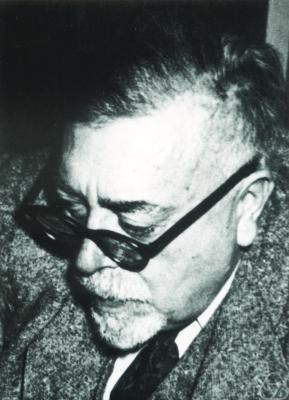
\includegraphics[height=0.42\textheight]{ch11_wiener.jpg}\\[1mm]
\imgcap{Norbert Wiener}
\imgcredit{https://commons.wikimedia.org/wiki/File:Norbert_wiener.jpg}{Photo: Konrad Jacobs, MFO; CC BY-SA 2.0 de; Wikimedia Commons}
\end{column}
\begin{column}{0.66\textwidth}
\begin{itemize}
    \item 1930: Wiener's generalised harmonic analysis; 1934: Khinchin; autocovariance and spectrum are a Fourier pair
    \item 1942: Cramér's representation of a stationary process as a random superposition of sinusoids
    \item 1961--1966: lag windows \refPar; the typical spectral shape of economic variables \refGra
    \item 1982: multitaper estimation \refTho; frequency-domain causality \refGew
    \item 1984--1989: wavelets \refGM, \refDau, \refMal; 1998: the practical guide \refTC
\end{itemize}
\end{column}
\end{columns}
\end{frame}

\begin{frame}{Known from TSA and new here}
\itemsize{\small}
\begin{itemize}
    \item Known (\atschlink{https://danpele.github.io/Time-Series-Analysis/EN/Courses/chapter12_spectral_analysis.pdf}{TSA, Chapter 12}): Fourier frequencies, the spectrum of ARMA models, the periodogram and its $\chi^2_2$ law, Daniell smoothing, tapering, Fisher's test, a first look at coherence and wavelets
    \item New: the research toolkit
    \begin{itemize}
        \item asymptotic theory of spectral estimators: bias, variance, optimal bandwidth, valid confidence bands, multitaper
        \item inference on co-movement: coherence thresholds, phase errors, dynamic correlation, causality by frequency
        \item filters judged by their gain; time--frequency analysis with significance tests that control false discoveries
    \end{itemize}
    \item Case studies: Thomson (1982), Croux--Forni--Reichlin (2001), Breitung--Candelon (2006), Baxter--King (1999), Cogley--Nason (1995), Hamilton (2018), Torrence--Compo (1998), Grinsted et al.\ (2004), with the specifications of the papers, on our data
\end{itemize}
\end{frame}


%=============================================================================
\section{The spectral representation}
%=============================================================================

\begin{frame}{Autocovariance and spectral distribution (1/2)}
\itemsize{\small}
\begin{itemize}
    \item \textbf{Herglotz} \refBD: $\gamma(\cdot)$ is the autocovariance of a stationary process if and only if
    \[ \gamma(h) = \int_{(-\pi, \pi]} e^{i\omega h}\,dF(\omega) \]
    \begin{itemize}
        \item $\gamma(h) = \Cov(X_{t+h}, X_t)$; $\omega$: angular frequency in radians per period; $F$: the \textbf{spectral distribution}, non-decreasing, right-continuous and bounded
    \end{itemize}
    \item If $\sum_h|\gamma(h)| < \infty$, $F$ has a density, the \textbf{spectral density}
    \[ dF(\omega) = f(\omega)\,d\omega, \qquad f(\omega) = \frac{1}{2\pi}\sum_h\gamma(h)e^{-i\omega h} \]
\end{itemize}
\end{frame}

\begin{frame}{Autocovariance and spectral distribution (2/2)}
\itemsize{\small}
\begin{itemize}
    \item At $h = 0$: the spectrum is a \textbf{decomposition of variance by frequency}
    \[ \gamma(0) = \Var(X_t) = \int_{-\pi}^{\pi}f(\omega)\,d\omega \]
    \begin{itemize}
        \item $f(\omega)\,d\omega$: the variance contributed by cycles with frequency near $\omega$; period $2\pi/\omega$
        \item quarterly data: the business-cycle band of 6--32 quarters is $\omega \in [\pi/16, \pi/3]$
    \end{itemize}
    \item A jump of $F$ at $\pm\omega_0$ is a deterministic cycle (a \textbf{line spectrum}); long memory is a pole of $f$ at $\omega = 0$ (\atschlink{https://danpele.github.io/Advanced-Time-Series/EN/Courses/chapter10_long_memory_rough_volatility.pdf}{Chapter 10})
\end{itemize}
\end{frame}

\begin{frame}{Cramér's representation}
\itemsize{\small}
\begin{columns}[T]
\begin{column}{0.32\textwidth}
\centering
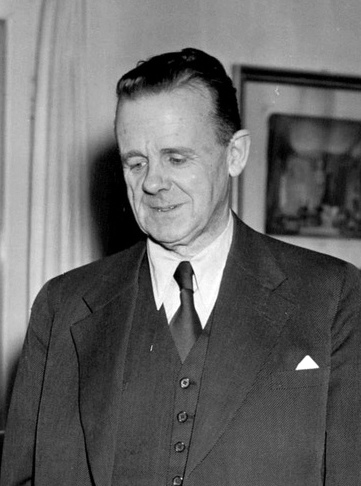
\includegraphics[height=0.4\textheight]{ch11_cramer_1951.jpg}\\[1mm]
\imgcap{Harald Cramér, 1951}
\imgcredit{https://commons.wikimedia.org/wiki/File:Harald_Cram\%C3\%A9r.jpg}{Photo: unknown photographer, Svenska Dagbladet (1951); public domain; Wikimedia Commons}
\end{column}
\begin{column}{0.66\textwidth}
\begin{itemize}
    \item Every zero-mean stationary process is a sum of sinusoids with random amplitudes \refBD
    \[ X_t = \int_{(-\pi, \pi]} e^{i\omega t}\,dZ(\omega) \]
    \begin{itemize}
        \item $dZ(\omega)$: the random amplitude at frequency $\omega$; $Z$ has \textbf{orthogonal increments}: $\E[dZ(\omega)\overline{dZ(\lambda)}] = 0$ for $\omega \ne \lambda$, $\E|dZ(\omega)|^2 = dF(\omega)$
    \end{itemize}
    \item Random amplitudes at different frequencies are uncorrelated: the frequency components can be studied one by one
    \item The discrete Fourier transform (DFT) $d(\omega_j) = n^{-1/2}\sum_t x_te^{-i\omega_jt}$ at $\omega_j = 2\pi j/n$ is the sample analogue of $dZ(\omega_j)$: nearly uncorrelated across Fourier frequencies
\end{itemize}
\end{column}
\end{columns}
\end{frame}

\begin{frame}{Linear filters in the frequency domain}
\itemsize{\small}
\begin{itemize}
    \item A linear filter multiplies each frequency component by the \textbf{transfer function} $A(\omega)$
    \[ Y_t = \sum_j a_jX_{t-j} \ \Rightarrow\ dZ_Y(\omega) = A(\omega)\,dZ_X(\omega), \quad A(\omega) = \sum_j a_je^{-i\omega j} \]
    \[ f_Y(\omega) = |A(\omega)|^2f_X(\omega) \]
    \begin{itemize}
        \item $a_j$: filter weights, $\sum_j|a_j| < \infty$; $|A(\omega)|$: the \textbf{gain}; $\arg A(\omega)$: the \textbf{phase shift}
        \item symmetric weights $a_j = a_{-j}$: $A(\omega)$ is real, no phase shift; the property every trend--cycle filter wants
    \end{itemize}
    \item First difference: $|1 - e^{-i\omega}|^2 = 2(1 - \cos\omega)$, zero at $\omega = 0$
    \begin{itemize}
        \item differencing removes the long cycles and amplifies the short ones
    \end{itemize}
    \item Slutsky effect: a moving sum of white noise has a peak in its spectrum, i.e.\ \textbf{cycles created by the filter}; the HP critique of Section 4 is the same phenomenon
\end{itemize}
\end{frame}

\begin{frame}{The spectral density matrix (1/2)}
\itemsize{\small}
\begin{itemize}
    \item Vector process $\mathbf X_t$ of dimension $k$: the Fourier transform of the autocovariance matrices
    \[ \mathbf f(\omega) = \frac{1}{2\pi}\sum_h\Gamma(h)e^{-i\omega h}, \qquad \Gamma(h) = \Cov(\mathbf X_{t+h}, \mathbf X_t) \]
    \begin{itemize}
        \item $\mathbf f(\omega)$: a $k \times k$ Hermitian ($\mathbf f = \mathbf f^*$, the conjugate transpose) non-negative definite matrix at each frequency
    \end{itemize}
    \item VARMA $\Phi(L)\mathbf X_t = \Theta(L)\boldsymbol\varepsilon_t$: the multivariate analogue of the ARMA spectrum
    \[ \mathbf f(\omega) = \frac{1}{2\pi}\Phi(e^{-i\omega})^{-1}\Theta(e^{-i\omega})\,\bSigma\,\Theta(e^{-i\omega})^*\Phi(e^{-i\omega})^{-*} \]
    \begin{itemize}
        \item $\Phi$, $\Theta$: matrix AR and MA polynomials; $\bSigma$: covariance of the innovations $\boldsymbol\varepsilon_t$; $^{-*}$: inverse of the conjugate transpose
    \end{itemize}
\end{itemize}
\end{frame}

\begin{frame}{The spectral density matrix (2/2): cross-spectra}
\itemsize{\small}
\begin{itemize}
    \item Off-diagonal elements: the \textbf{cross-spectrum}, complex-valued
    \[ f_{xy}(\omega) = c_{xy}(\omega) - i\,q_{xy}(\omega) \]
    \begin{itemize}
        \item $c_{xy}$: co-spectrum, even in $\omega$ (contemporaneous co-movement), $\int c_{xy} = \Cov(X_t, Y_t)$
        \item $q_{xy}$: quadrature spectrum, odd in $\omega$ (lead--lag between the series)
    \end{itemize}
    \item Section 2 estimates the diagonal, Section 3 the off-diagonal, Section 4 factorises $\mathbf f$ to measure causality
\end{itemize}
\end{frame}

\begin{frame}{Variance by frequency band}
\itemsize{\footnotesize}
\begin{center}
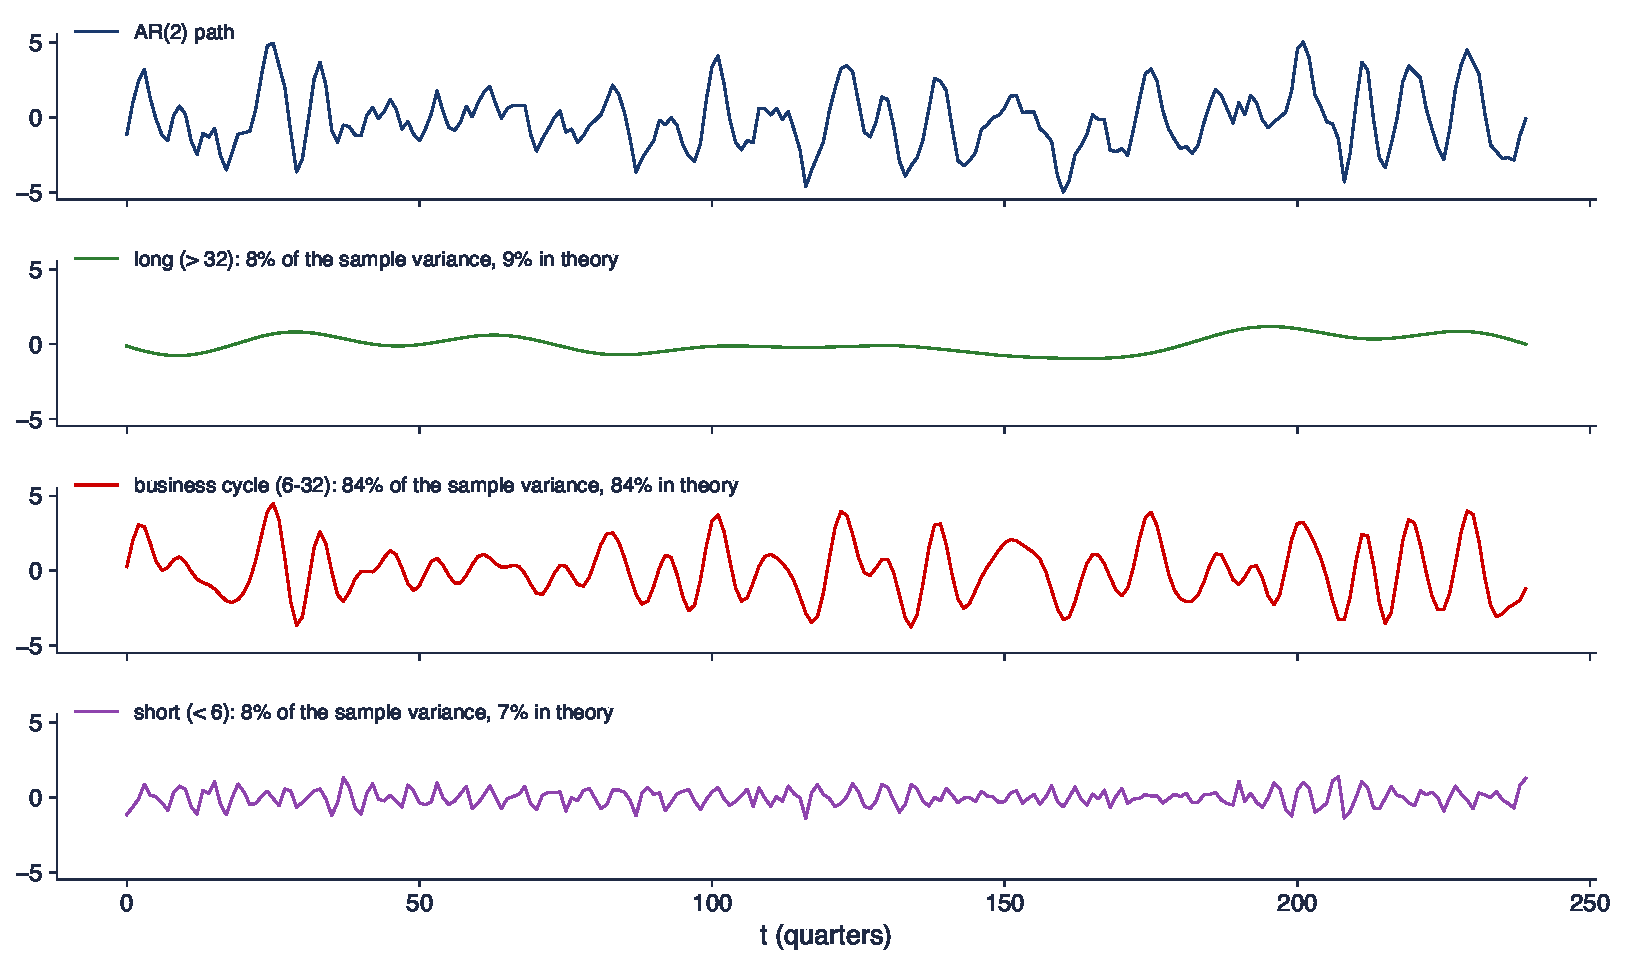
\includegraphics[width=0.97\textwidth,height=0.52\textheight,keepaspectratio]{ats_ch11_bands.pdf}
\end{center}
\vspace{-0.25cm}
\begin{itemize}
    \item An AR(2) path, $X_t = 1.3X_{t-1} - 0.7X_{t-2} + \varepsilon_t$, 240 ``quarters'', split by the DFT into three bands; shares of variance in the sample and $2\int_{\mathrm{band}}f/\gamma(0)$ in theory
\end{itemize}
\quantlet{ATS\_ch11\_spectral\_estimation}{\qlurl{ATS_ch11_spectral_estimation}}
\end{frame}

\begin{frame}{Interpreting the band decomposition}
\itemsize{\small}
\begin{itemize}
    \item The spectral peak is at a period of 9.5: 84\% of the variance lies in the band of 6--32 periods (sample: 84\%)
    \item Long and short cycles carry 9\% and 7\% in theory: the three components are uncorrelated by Cramér's theorem, so the shares add up
    \item The ``business cycle'' of an AR(2) is a stochastic pseudo-cycle: irregular amplitude and length, no line in the spectrum
    \item Band-pass filters (Section 4) estimate exactly this middle component from a finite sample
\end{itemize}
\end{frame}

\begin{frame}{Recap: The spectral representation}
\itemsize{\small}
\begin{itemize}
    \item The spectrum decomposes variance by frequency; Cramér: uncorrelated random amplitudes at each frequency
    \item A linear filter multiplies the spectrum by its squared gain; symmetric filters do not shift phase
    \item The spectral matrix contains cross-spectra: co-movement and lead--lag by frequency
\end{itemize}
\end{frame}


%=============================================================================
\section{Spectral estimation theory}
%=============================================================================

\begin{frame}{Why the periodogram is not enough}
\itemsize{\small}
\begin{itemize}
    \item For a linear process the periodogram ordinates are asymptotically scaled $\chi^2_2$ variables \refBD
    \[ X_t = \sum_j\psi_j\varepsilon_{t-j} \ \Rightarrow\ I(\omega_j) \Rightarrow f(\omega_j)\,\frac{\chi^2_2}{2} \]
    \begin{itemize}
        \item $\psi_j$: weights with $\sum_j|j|^{1/2}|\psi_j| < \infty$; $\varepsilon_t$: i.i.d. innovations; $f > 0$; asymptotically independent over fixed Fourier frequencies $\omega_j$
        \item $\E I(\omega_j) \to f(\omega_j)$ but $\Var I(\omega_j) \to f(\omega_j)^2$: \textbf{inconsistent}, the variance does not fall with $n$
    \end{itemize}
    \item Leakage: the mean periodogram is the true spectrum smoothed by the Fejér kernel $F_n$
    \[ \E I(\omega) = \int F_n(\omega - \lambda)f(\lambda)\,d\lambda \]
    \begin{itemize}
        \item the side lobes of $F_n$ decay only like $1/(n\omega^2)$, so power \textbf{leaks} from strong to weak frequencies
    \end{itemize}
    \item Two remedies: \textbf{average} neighbouring frequencies (consistency) and \textbf{taper} the data (bias); multitaper does both
\end{itemize}
\end{frame}

\begin{frame}{Lag-window estimators (1/2)}
\itemsize{\small}
\begin{itemize}
    \item Down-weight the noisy sample autocovariances at long lags \refPar
    \[ \hat f(\omega) = \frac{1}{2\pi}\sum_{|h| < n}k(h/M)\,\hat\gamma(h)e^{-i\omega h} \]
    \begin{itemize}
        \item $\hat\gamma(h)$: sample autocovariance; $k$: the \textbf{lag window}, $k(0) = 1$, decreasing in $|u|$; $M$: the truncation (bandwidth) parameter
    \end{itemize}
    \item Equivalently: a weighted average of the periodogram with the \textbf{spectral window} $W_M$
    \[ \hat f(\omega) = \int W_M(\omega - \lambda)I(\lambda)\,d\lambda, \qquad W_M(\omega) = \frac{1}{2\pi}\sum_h k(h/M)e^{-i\omega h} \]
    \begin{itemize}
        \item a large $M$ gives a narrow $W_M$: little smoothing
    \end{itemize}
\end{itemize}
\end{frame}

\begin{frame}{Lag-window estimators (2/2): the kernels}
\itemsize{\small}
\begin{itemize}
    \item Bartlett $k(u) = 1 - |u|$; Parzen; Tukey--Hanning; quadratic spectral (QS): the same kernels as the HAC estimators of \atschlink{https://danpele.github.io/Advanced-Time-Series/EN/Courses/chapter0_refresher_inference.pdf}{Chapter 0} at $\omega = 0$
    \begin{itemize}
        \item a non-negative $W_M$ guarantees $\hat f \ge 0$ (Bartlett, Parzen, QS); Tukey--Hanning can go negative
    \end{itemize}
    \item Characteristic exponent $q$: how flat the kernel is at zero
    \[ k_q = \lim_{u \to 0}\frac{1 - k(u)}{|u|^q} \]
    \begin{itemize}
        \item Bartlett $q = 1$, $k_1 = 1$; Parzen $q = 2$, $k_2 = 6$; QS $q = 2$, $k_2 = 1.42$; a larger $q$ means smaller bias (next slides)
    \end{itemize}
\end{itemize}
\end{frame}

\begin{frame}{Lag windows and spectral windows}
\itemsize{\footnotesize}
\begin{center}
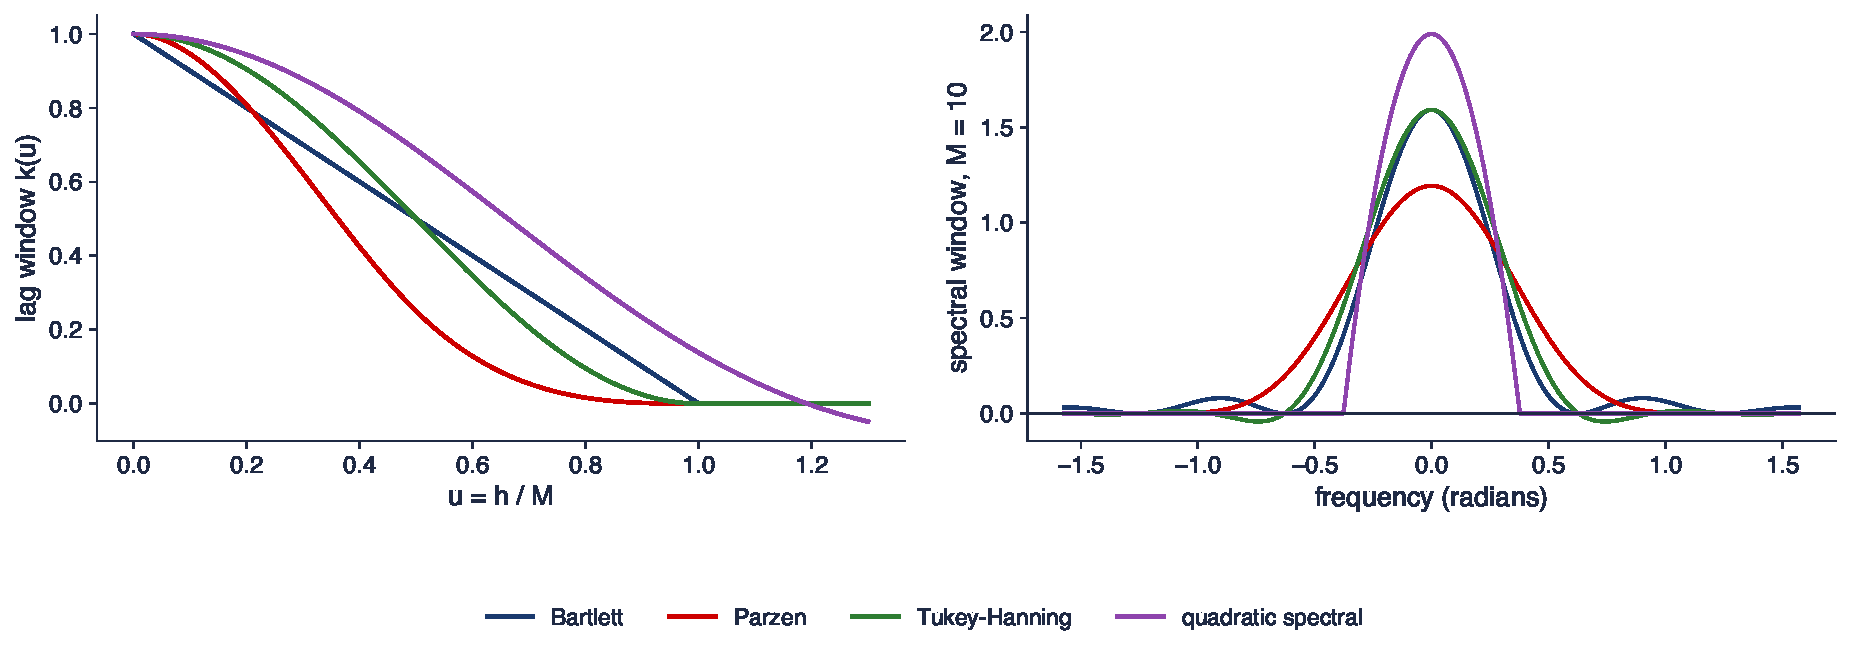
\includegraphics[width=0.97\textwidth,height=0.5\textheight,keepaspectratio]{ats_ch11_kernels.pdf}
\end{center}
\vspace{-0.25cm}
\begin{itemize}
    \item Left: $k(u)$; right: the spectral window $W_M(\omega)$ for $M = 10$, the weights that each estimator gives to the periodogram around $\omega$
\end{itemize}
\quantlet{ATS\_ch11\_spectral\_estimation}{\qlurl{ATS_ch11_spectral_estimation}}
\end{frame}

\begin{frame}{Interpreting the windows}
\itemsize{\small}
\begin{itemize}
    \item A narrow $W_M$ means low bias and high variance; Parzen is the widest at $M = 10$ (its $\int k^2 = 0.54$ is the smallest), QS the narrowest
    \item Bartlett has side lobes (leakage through the window itself); Tukey--Hanning has negative weights
    \item Comparing kernels at the same $M$ is misleading: compare them at the same variance (the same equivalent degrees of freedom)
    \item The QS kernel is optimal in MSE among kernels with non-negative estimates \refAnd
\end{itemize}
\end{frame}

\begin{frame}{Bias, variance and the optimal bandwidth (1/2)}
\itemsize{\small}
\begin{itemize}
    \item If $M \to \infty$ and $M/n \to 0$: $\hat f(\omega) \to_p f(\omega)$ (\textbf{consistency}) \refPar; variance and bias
    \[ \Var\hat f(\omega) \approx \frac{M}{n}f(\omega)^2\int k^2(u)\,du, \qquad \E\hat f(\omega) - f(\omega) \approx -k_qM^{-q}f^{(q)}(\omega) \]
    \begin{itemize}
        \item the variance grows with $M$ (doubled at $\omega = 0, \pm\pi$); the bias falls with $M$
        \item $f^{(q)}(\omega) = \frac{1}{2\pi}\sum_h|h|^q\gamma(h)e^{-i\omega h}$: a generalised $q$-th derivative of $f$, large where the spectrum is curved (peaks)
    \end{itemize}
\end{itemize}
\end{frame}

\begin{frame}{Bias, variance and the optimal bandwidth (2/2)}
\itemsize{\small}
\begin{itemize}
    \item Minimising MSE = squared bias + variance over $M$
    \[ M^* = \Big(\frac{qk_q^2f^{(q)}(\omega)^2\,n}{f(\omega)^2\int k^2}\Big)^{1/(2q+1)} \propto n^{1/(2q+1)}, \qquad \mathrm{MSE} \propto n^{-2q/(2q+1)} \]
    \begin{itemize}
        \item $q = 2$ kernels converge faster ($n^{-4/5}$) than Bartlett ($n^{-2/3}$)
    \end{itemize}
    \item Inference: a scaled $\chi^2$ with equivalent degrees of freedom $\nu$
    \[ \frac{\nu\hat f(\omega)}{f(\omega)} \approx \chi^2_\nu, \qquad \nu = \frac{2n}{M\int k^2} \]
    \begin{itemize}
        \item the confidence band $[\nu\hat f/\chi^2_{\nu,0.975}, \nu\hat f/\chi^2_{\nu,0.025}]$ has constant width in log scale
    \end{itemize}
\end{itemize}
\end{frame}

\begin{frame}{The bias--variance trade-off at a spectral peak}
\itemsize{\footnotesize}
\begin{center}
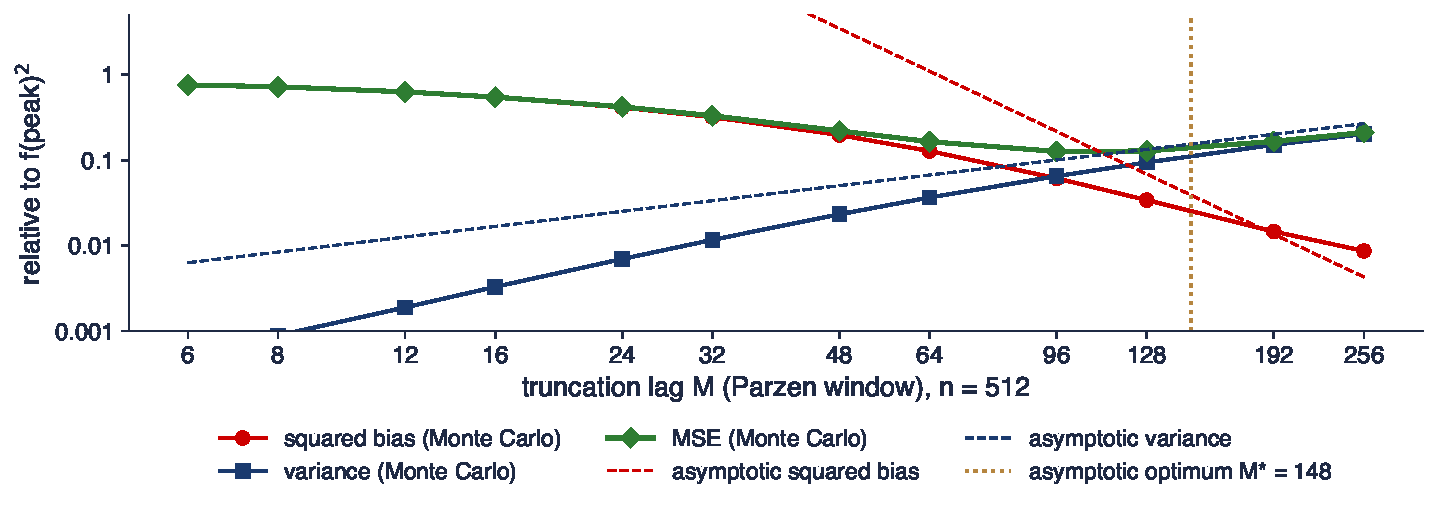
\includegraphics[width=0.97\textwidth,height=0.5\textheight,keepaspectratio]{ats_ch11_bias_variance.pdf}
\end{center}
\vspace{-0.25cm}
\begin{itemize}
    \item Parzen estimator at the peak (period 11.1) of $X_t = 1.6X_{t-1} - 0.9X_{t-2} + \varepsilon_t$, $n = 512$, 400 simulations; curves divided by $f(\mathrm{peak})^2$; dashed: the asymptotic formulas
\end{itemize}
\quantlet{ATS\_ch11\_spectral\_estimation}{\qlurl{ATS_ch11_spectral_estimation}}
\end{frame}

\begin{frame}{Interpreting the trade-off}
\itemsize{\small}
\begin{itemize}
    \item With $M = 12$ the relative RMSE is 0.79, almost all of it bias (0.79): heavy smoothing flattens the peak
    \item The Monte Carlo optimum is $M = 96$ (relative RMSE 0.36); the asymptotic formula gives $M^* = 148$: same order, but the formula ignores higher-order bias terms
    \item The asymptotic variance is accurate only once the window is narrower than the peak; the asymptotic bias explodes for small $M$
    \item A sharp spectral peak needs a much larger $M$ than the HAC rule for $\omega = 0$ would suggest: bandwidth is local
\end{itemize}
\end{frame}

\begin{frame}{Choosing the bandwidth}
\itemsize{\small}
\begin{itemize}
    \item \textbf{Plug-in} \refAnd: approximate $f^{(q)}/f$ by a parametric (AR(1)) model, then use $M^*$
    \[ M = 1.1447\,(\hat\alpha(1)\,n)^{1/3} \ \text{(Bartlett)}, \qquad M = 1.3221\,(\hat\alpha(2)\,n)^{1/5} \ \text{(QS)}, \qquad \omega = 0 \]
    \begin{itemize}
        \item $\hat\alpha(q)$: the ratio $(f^{(q)}(0)/f(0))^2$ computed from the fitted AR(1), e.g.\ $\hat\alpha(2) = 4\hat\rho^2/(1 - \hat\rho)^4$ ($\hat\rho$: AR coefficient)
        \item good for long-run variances (\atschlink{https://danpele.github.io/Advanced-Time-Series/EN/Courses/chapter0_refresher_inference.pdf}{Chapter 0}); poor near sharp peaks, where the AR(1) approximation is wrong
    \end{itemize}
    \item \textbf{Cross-validation} \refHur: minimise over $M$ a leave-one-out Whittle criterion
    \[ \mathrm{CV}(M) = \sum_j\Big[\log\hat f_{-j}(\omega_j) + \frac{I(\omega_j)}{\hat f_{-j}(\omega_j)}\Big] \]
    \begin{itemize}
        \item $\hat f_{-j}$: the smoothed estimate computed without the ordinate $I(\omega_j)$
    \end{itemize}
    \item \textbf{Resolution}: two peaks closer than the bandwidth (about $1/M$ cycles) merge; decide the resolution you need before looking at the data
    \begin{itemize}
        \item report the estimate for two or three bandwidths: conclusions that depend on $M$ are not conclusions
    \end{itemize}
\end{itemize}
\end{frame}

\begin{frame}{Multitaper estimation (1/2): Slepian tapers}
\itemsize{\small}
\begin{itemize}
    \item \textbf{Slepian (DPSS) tapers} $v^{(k)}$, $k = 0, \dots, K - 1$ \refTho
    \begin{itemize}
        \item orthonormal weight sequences of length $n$ that maximise the share $\lambda_k$ of their spectral energy inside $[-W, W]$; $W$: half-bandwidth in cycles
        \item about $2nW$ of them have $\lambda_k \approx 1$; usually $K = 2NW - 1$ with $NW = nW$ (e.g.\ $NW = 4$, $K = 7$)
    \end{itemize}
    \item Eigenspectra: one tapered periodogram per taper; the estimate is their average
    \[ \hat S_k(\omega) = \frac{1}{2\pi}\Big|\sum_tv_t^{(k)}x_te^{-i\omega t}\Big|^2, \qquad \hat f^{\mathrm{mt}}(\omega) = \frac1K\sum_{k=0}^{K-1}\hat S_k(\omega) \]
    \begin{itemize}
        \item the $\hat S_k$ are nearly uncorrelated: $2K\hat f^{\mathrm{mt}}/f \approx \chi^2_{2K}$; variance $f^2/K$, bias controlled by the taper concentration
    \end{itemize}
\end{itemize}
\end{frame}

\begin{frame}{Multitaper estimation (2/2): adaptive weights}
\itemsize{\small}
\begin{itemize}
    \item \textbf{Adaptive weights} \refPWa: down-weight leaky tapers where $f$ is small
    \[ d_k(\omega) = \frac{\sqrt{\lambda_k}\,f(\omega)}{\lambda_kf(\omega) + (1 - \lambda_k)\sigma^2} \]
    \begin{itemize}
        \item $\sigma^2$: the variance of the series; $1 - \lambda_k$: the leakage of taper $k$; the weights depend on the unknown $f$, so they are iterated from $\hat f^{\mathrm{mt}}$
    \end{itemize}
    \item Alternatives with the same logic: sine tapers \refRS; Welch's averaging of tapered segments \refWel
\end{itemize}
\end{frame}

\begin{frame}{Slepian tapers}
\itemsize{\footnotesize}
\begin{center}
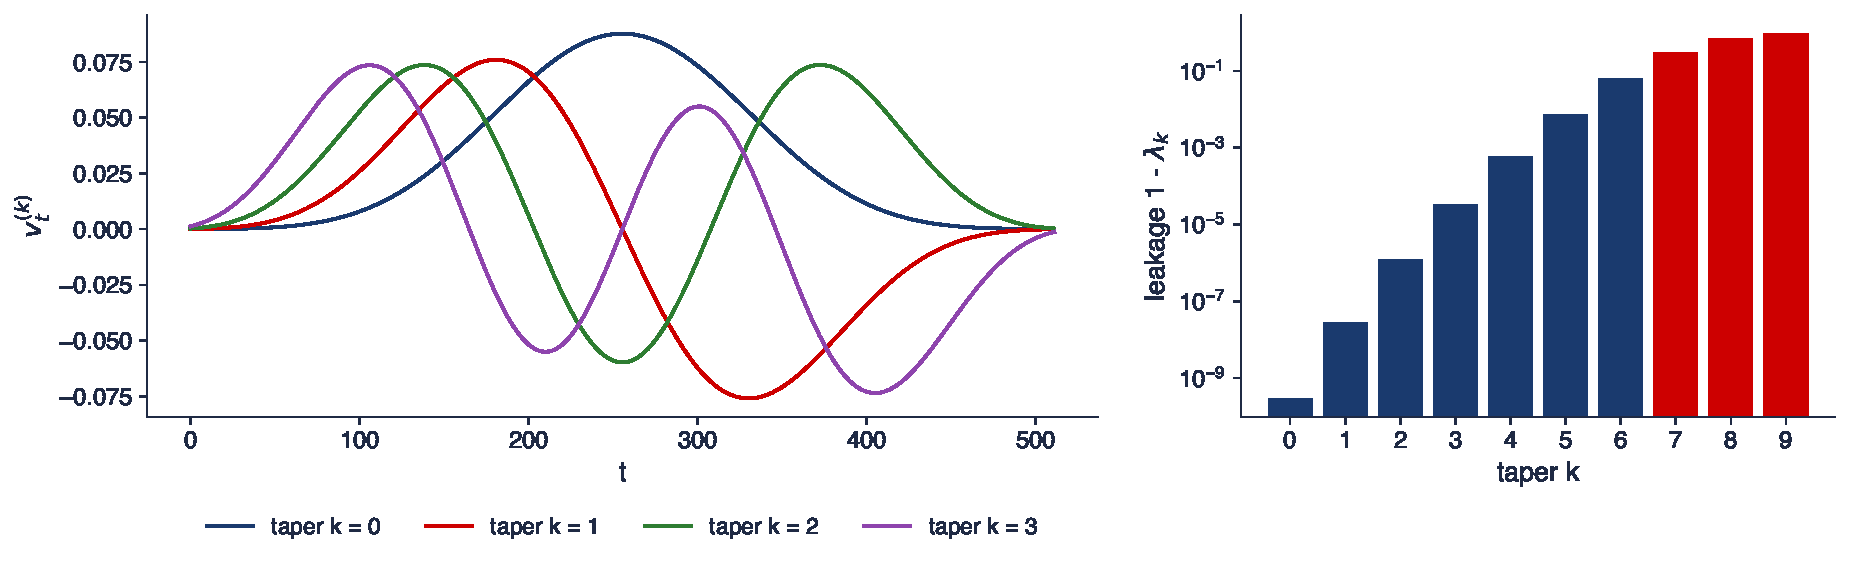
\includegraphics[width=0.97\textwidth,height=0.48\textheight,keepaspectratio]{ats_ch11_dpss.pdf}
\end{center}
\vspace{-0.25cm}
\begin{itemize}
    \item $n = 512$, $NW = 4$: the first four tapers and the leakage $1 - \lambda_k$ of the first ten (blue: $k < 2NW - 1$)
\end{itemize}
\quantlet{ATS\_ch11\_spectral\_estimation}{\qlurl{ATS_ch11_spectral_estimation}}
\end{frame}

\begin{frame}{Interpreting the tapers}
\itemsize{\small}
\begin{itemize}
    \item Taper $k$ has $k$ zero crossings: higher tapers weight the ends of the sample, so together they use all the data
    \item Leakage grows fast with $k$: $\lambda_6 = 0.937$, but $\lambda_7 = 0.70$ and $\lambda_8 = 0.30$; beyond $2NW - 1$ the tapers are useless
    \item The single Hann taper throws away the ends; multitapering recovers that information as extra degrees of freedom
    \item $NW$ is the only tuning choice: it fixes the resolution $2W = 2NW/n$ and the variance $f^2/K$ together
\end{itemize}
\end{frame}

\begin{frame}{Leakage on a spectrum with a high dynamic range}
\itemsize{\footnotesize}
\begin{center}
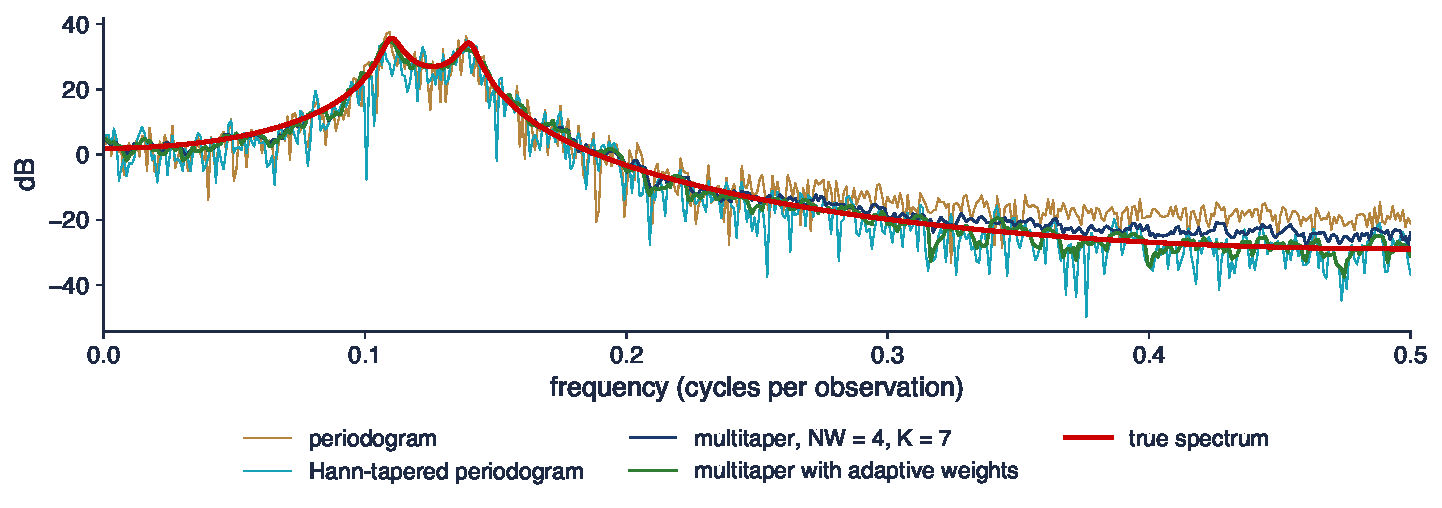
\includegraphics[width=0.97\textwidth,height=0.5\textheight,keepaspectratio]{ats_ch11_leakage.pdf}
\end{center}
\vspace{-0.25cm}
\begin{itemize}
    \item The AR(4) of Percival and Walden (1993), $n = 1024$, range of 65 dB between peak and trough; one simulated path (median leakage of 21)
\end{itemize}
\quantlet{ATS\_ch11\_spectral\_estimation}{\qlurl{ATS_ch11_spectral_estimation}}
\end{frame}

\begin{frame}{Interpreting leakage}
\itemsize{\small}
\begin{itemize}
    \item Mean bias at frequencies above 0.3 cycles (200 simulations): periodogram +11.2 dB, Hann taper \ensuremath{-}2.5 dB, multitaper +6.3 dB, adaptive multitaper \ensuremath{-}0.8 dB
    \item The raw periodogram fills the trough with power leaked from the peaks: averaging it more would not help, the bias is in each ordinate
    \item With equal weights the leaky high-order tapers still contaminate the trough; the adaptive weights remove it
    \item Economic data rarely have 60 dB ranges, but spectra of levels with a unit-root-like peak at zero do: taper or prewhiten before estimating
\end{itemize}
\end{frame}

\begin{frame}{Five estimators in a Monte Carlo}
\itemsize{\footnotesize}
\begin{center}
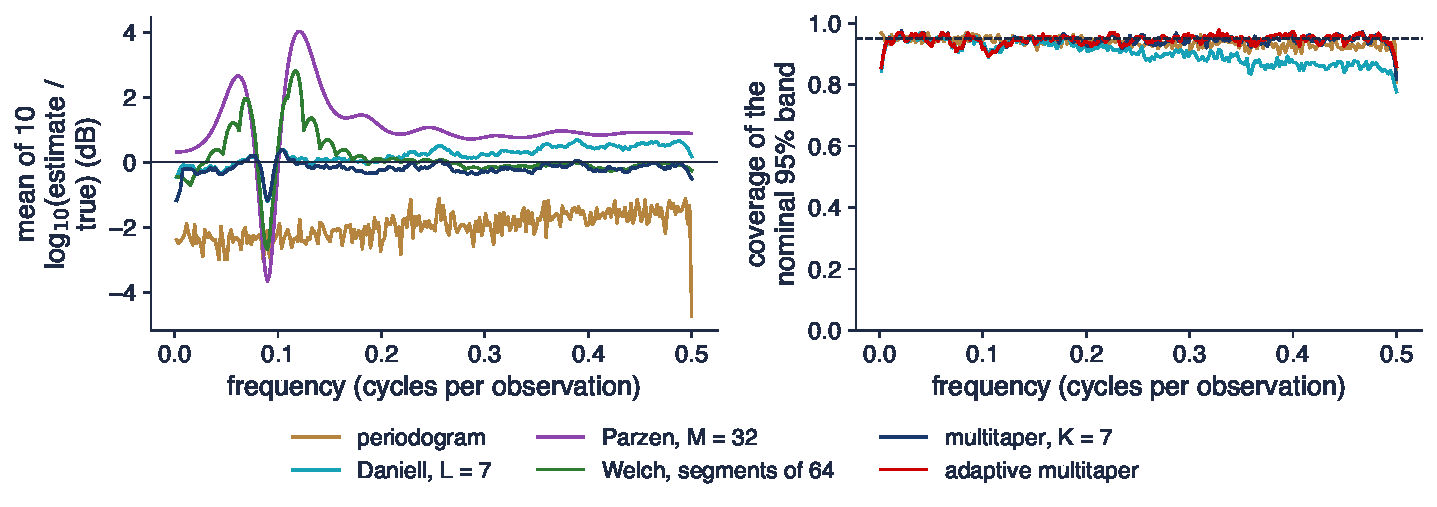
\includegraphics[width=0.97\textwidth,height=0.5\textheight,keepaspectratio]{ats_ch11_mt_mc.pdf}
\end{center}
\vspace{-0.25cm}
\begin{itemize}
    \item $X_t = 1.6X_{t-1} - 0.9X_{t-2} + \varepsilon_t$, $n = 512$, 400 simulations: mean log-bias by frequency and coverage of the nominal 95\% $\chi^2$ bands
\end{itemize}
\quantlet{ATS\_ch11\_spectral\_estimation}{\qlurl{ATS_ch11_spectral_estimation}}
\end{frame}

\begin{frame}{Interpreting the Monte Carlo}
\itemsize{\small}
\begin{itemize}
    \item Standard deviation of $10\log_{10}(\hat f/f)$: periodogram 5.6 dB, Daniell 1.8, multitaper 1.7, Parzen 0.9, Welch 1.1
    \item At the peak: Parzen \ensuremath{-}2.3 dB, Welch \ensuremath{-}1.4 dB, multitaper \ensuremath{-}0.5 dB; the periodogram's \ensuremath{-}2.0 dB is the mean of $\log\chi^2_2/2$, not a bias in levels
    \item Coverage of the 95\% band: multitaper 94.3\%, adaptive 94.6\%, Daniell 90.3\% (its band ignores the bias on the slopes)
    \item Multitaper is the only estimator here with small bias, small variance and honest bands at once
\end{itemize}
\end{frame}

\begin{frame}{Industrial production: Romania and the euro area}
\itemsize{\footnotesize}
\begin{center}
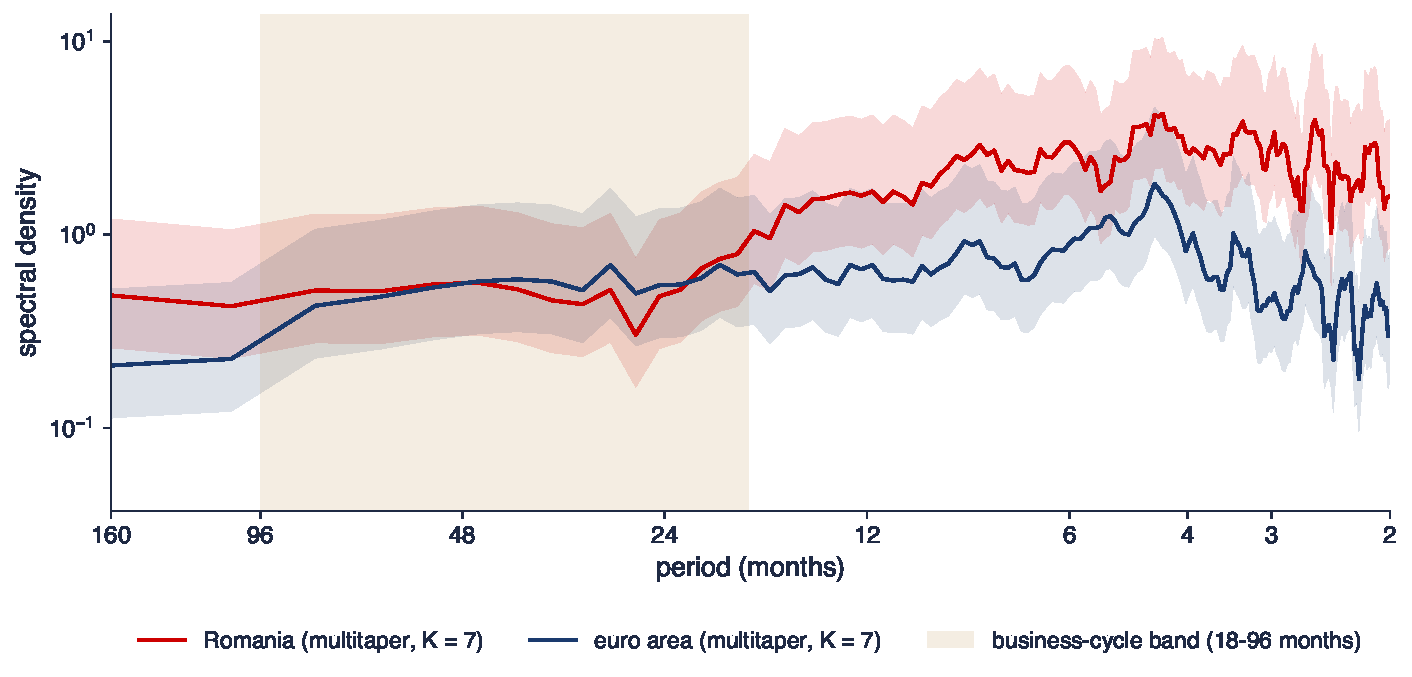
\includegraphics[width=0.97\textwidth,height=0.5\textheight,keepaspectratio]{ats_ch11_ip_spectrum.pdf}
\end{center}
\vspace{-0.25cm}
\begin{itemize}
    \item Monthly growth of industrial production (seasonally and calendar adjusted), February 2000 -- July 2026, 318 months; multitaper $NW = 4$ with 95\% bands
\end{itemize}
\quantlet{ATS\_ch11\_ip\_spectrum}{\qlurl{ATS_ch11_ip_spectrum}}
\end{frame}

\begin{frame}{Interpreting the industrial production spectra}
\itemsize{\small}
\begin{itemize}
    \item Monthly growth is dominated by short periods: cycles under 6 months carry 77\% of the variance in Romania and 69\% in the euro area
    \item The business-cycle band (18--96 months) holds 2.1\% (Romania) and 7.3\% (euro area): growth rates hide cycles that levels show (the first-difference gain)
    \item Romania is more volatile (standard deviation 3.61 against 1.98), and the excess is at high frequencies, where the bands do not overlap: noise, revisions and residual calendar effects
    \item At periods above 12 months the two spectra cannot be told apart within the bands
\end{itemize}
\end{frame}

\begin{frame}{Lines in the spectrum: Thomson's F test (1/2)}
\itemsize{\small}
\begin{itemize}
    \item Model: a sinusoid plus noise with a smooth spectrum \refTho
    \[ x_t = \mu\cos(\omega_0t + \phi) + e_t \]
    \begin{itemize}
        \item $\mu$: amplitude; $\omega_0$: frequency of the line; $\phi$: phase; $e_t$: stationary noise
        \item under a line, each tapered DFT is $Y_k(\omega_0) \approx \mu\,U_k(0)$, with $U_k(0) = \sum_tv^{(k)}_t$ the sum of taper $k$
    \end{itemize}
    \item A regression of the eigencoefficients $Y_k$ on the taper sums $U_k(0)$, frequency by frequency: it separates a deterministic line from a stochastic peak, which Fisher's test (TSA) cannot
\end{itemize}
\end{frame}

\begin{frame}{Lines in the spectrum: Thomson's F test (2/2)}
\itemsize{\small}
\begin{itemize}
    \item Estimated amplitude and the F statistic: explained against residual variation
    \[ \hat\mu(\omega) = \frac{\sum_kU_k(0)Y_k(\omega)}{\sum_kU_k(0)^2}, \qquad F(\omega) = \frac{(K - 1)\,|\hat\mu|^2\sum_kU_k(0)^2}{\sum_k|Y_k - \hat\mu U_k(0)|^2} \sim F_{2, 2K - 2} \]
    \begin{itemize}
        \item a large $F(\omega)$: a line at $\omega$; $K$: number of tapers
    \end{itemize}
    \item Application: residual seasonality is a set of lines at $k/12$ cycles per month; trading-day effects are lines at 0.348 and 0.432 cycles per month
    \item Testing at hundreds of frequencies: expect about 1\% false rejections at the 1\% level; test only pre-specified frequencies
\end{itemize}
\end{frame}

\begin{frame}{Residual seasonality in Romanian industrial production}
\itemsize{\footnotesize}
\begin{center}
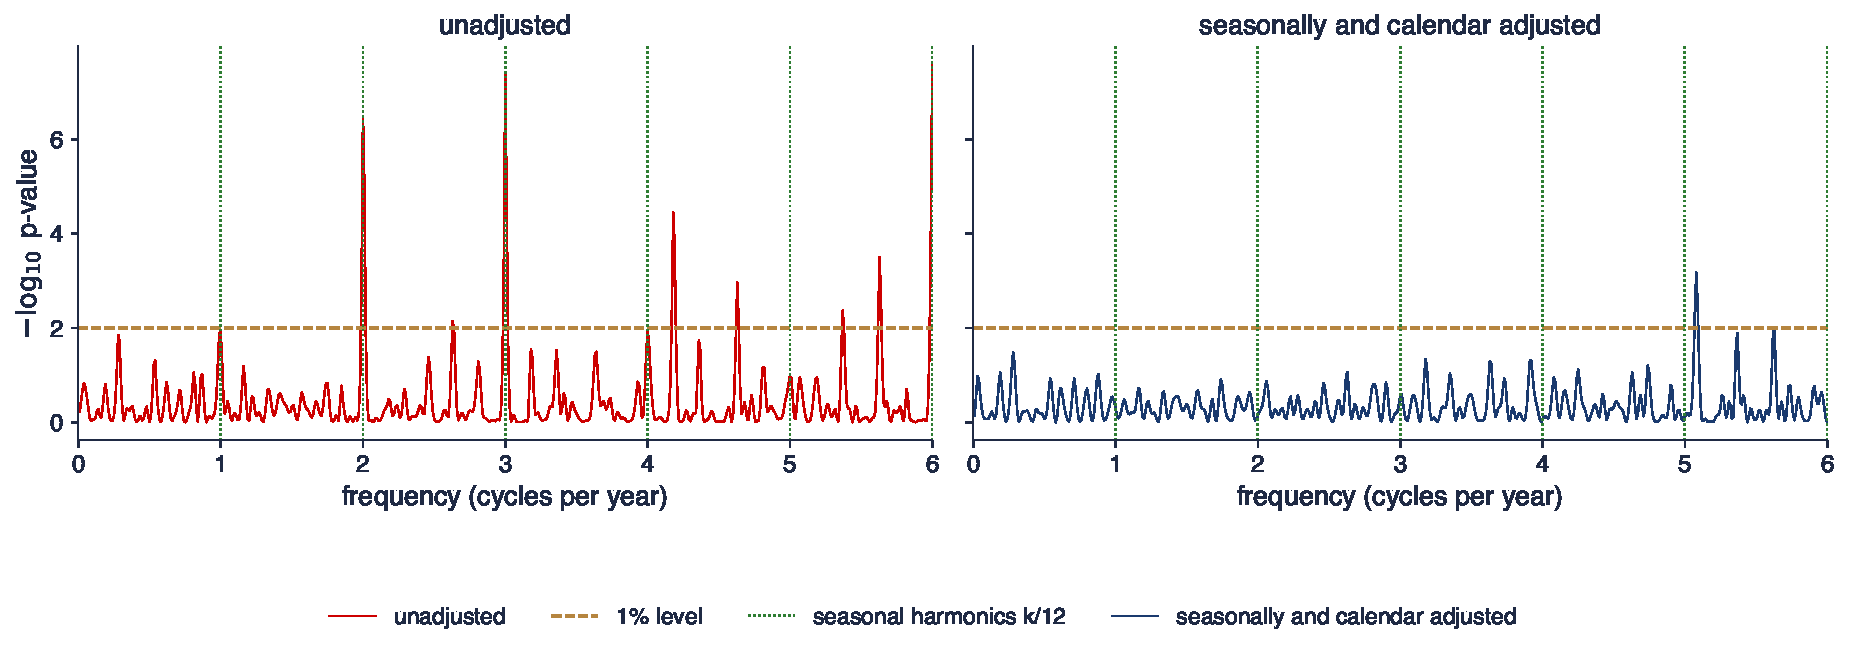
\includegraphics[width=0.97\textwidth,height=0.5\textheight,keepaspectratio]{ats_ch11_ftest.pdf}
\end{center}
\vspace{-0.25cm}
\begin{itemize}
    \item Harmonic F test ($NW = 4$, $K = 7$) on monthly growth, unadjusted and adjusted series; dotted lines: the six seasonal frequencies
\end{itemize}
\quantlet{ATS\_ch11\_ip\_spectrum}{\qlurl{ATS_ch11_ip_spectrum}}
\end{frame}

\begin{frame}{Interpreting the F test}
\itemsize{\small}
\begin{itemize}
    \item Unadjusted: 3 of 6 seasonal harmonics are lines at 1\% ($p$ $<$ 0.0001 and $<$ 0.0001 at 2 and 3 cycles per year); the annual harmonic is borderline ($p$ = 0.012)
    \item A strong line at 4.18 cycles per year ($p$ $<$ 0.0001): the trading-day frequency, a calendar effect, not seasonality
    \item Adjusted series: none of the six harmonics is significant, and there is no line at the trading-day frequency ($p$ = 0.22): the adjustment passes this check
    \item The annual harmonic is weak because Romanian seasonality is not a pure sinusoid: its power sits at the higher harmonics
\end{itemize}
\end{frame}

\begin{frame}{Recap: Spectral estimation theory}
\itemsize{\small}
\begin{itemize}
    \item The periodogram is unbiased in the limit but inconsistent and leaky; smoothing buys consistency, tapering buys low bias
    \item Bandwidth is a bias--variance choice with $M^* \propto n^{1/(2q+1)}$; peaks need narrow windows
    \item Multitaper: $\chi^2_{2K}$ bands that hold, adaptive weights against leakage, and an F test for lines
\end{itemize}
\end{frame}


%=============================================================================
\section{Two series: coherence, phase and causality}
%=============================================================================

\begin{frame}{Coherence, phase and gain (1/2): coherence}
\itemsize{\small}
\begin{itemize}
    \item \textbf{Squared coherence}: the $R^2$ of the regression of $dZ_y(\omega)$ on $dZ_x(\omega)$
    \[ \kappa^2_{xy}(\omega) = \frac{|f_{xy}(\omega)|^2}{f_x(\omega)f_y(\omega)} \in [0, 1] \]
    \begin{itemize}
        \item $f_x$, $f_y$: the two spectra; $f_{xy}$: the cross-spectrum; $\kappa^2 = 1$: $y$ is an exact linear filter of $x$ at frequency $\omega$; $\kappa^2 = 0$: no linear relation at that frequency
        \item invariant to filtering each series by an invertible filter: coherence does not depend on how the series are transformed (\atsapplink{atsapp2}{atssrc1}{Appendix})
    \end{itemize}
    \item \textbf{Gain} $|f_{xy}(\omega)|/f_x(\omega)$: the regression coefficient of $y$ on $x$ at frequency $\omega$
\end{itemize}
\end{frame}

\begin{frame}{Coherence, phase and gain (2/2): phase}
\itemsize{\small}
\begin{itemize}
    \item \textbf{Phase}: the angle of the cross-spectrum, with $\gamma_{xy}(h) = \Cov(x_{t+h}, y_t)$
    \[ \phi_{xy}(\omega) = \arg f_{xy}(\omega) \]
    \begin{itemize}
        \item example: if $y_t = x_{t-d}$, then $f_{xy} = e^{i\omega d}f_x$, phase $\omega d > 0$: $x$ leads by $\phi/\omega$ periods
        \item the phase is defined modulo $2\pi$: a lead of $d$ and a lag of $2\pi/\omega - d$ are the same phase
    \end{itemize}
    \item Interpret the phase only where coherence is significant
\end{itemize}
\end{frame}

\begin{frame}{Inference on coherence and phase}
\itemsize{\small}
\begin{itemize}
    \item The raw cross-periodogram gives $\hat\kappa^2 \equiv 1$ at every frequency: coherence \textbf{must} be smoothed (here: averaged over $K$ tapers)
    \[ \Pr(\hat\kappa^2 > c \mid \kappa^2 = 0) = (1 - c)^{L-1} \ \Rightarrow\ c_{0.05} = 1 - 0.05^{1/(L-1)} \]
    \begin{itemize}
        \item $L$: number of independent ordinates averaged ($L = K$ for multitaper); $c$: threshold; $\hat\kappa^2$ above $c_{0.05}$ is significant at 5\%
    \end{itemize}
    \item $\hat\kappa^2$ is biased upwards when $\kappa^2$ is small; confidence intervals via the Fisher transform $\tanh^{-1}\hat\kappa$ \refSS
    \begin{itemize}
        \item phase: $\mathrm{se}(\hat\phi) \approx \sqrt{(1/\hat\kappa^2 - 1)/(2L)}$; it explodes as coherence falls
    \end{itemize}
    \item Misalignment bias: a long delay $d$ rotates the phase within the smoothing band and lowers $\hat\kappa^2$; align the series (or prewhiten) first
\end{itemize}
\end{frame}

\begin{frame}{Romania and the euro area: coherence, phase and gain}
\itemsize{\footnotesize}
\begin{center}
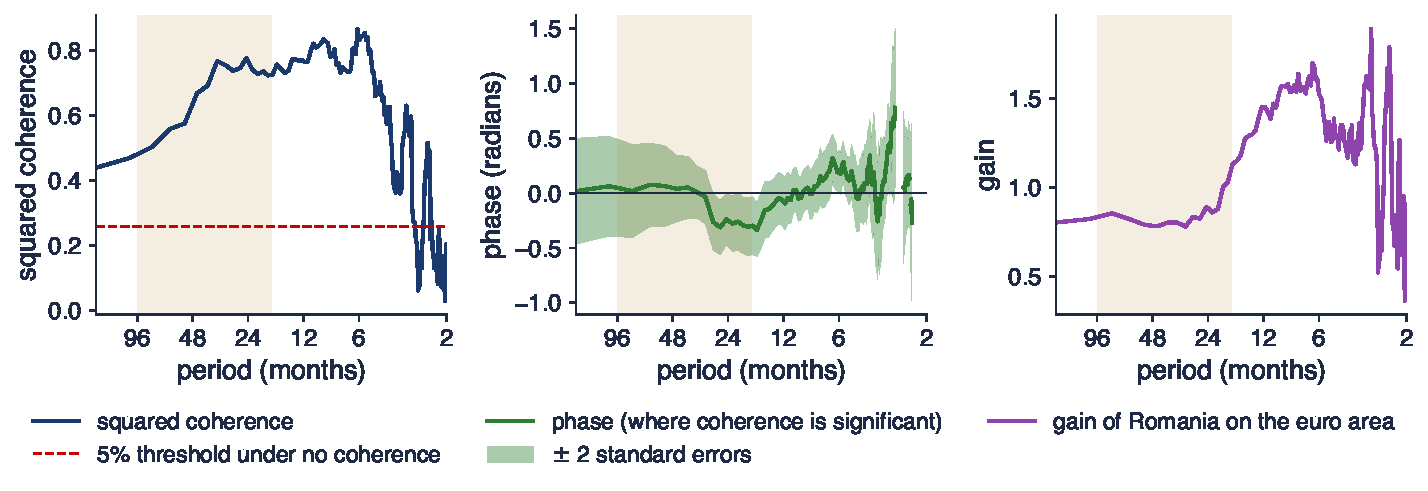
\includegraphics[width=0.97\textwidth,height=0.48\textheight,keepaspectratio]{ats_ch11_coherence.pdf}
\end{center}
\vspace{-0.25cm}
\begin{itemize}
    \item Monthly industrial production growth, euro area ($x$) and Romania ($y$); multitaper $NW = 6$, $K = 11$; shaded: 18--96 months
\end{itemize}
\quantlet{ATS\_ch11\_cross\_spectrum}{\qlurl{ATS_ch11_cross_spectrum}}
\end{frame}

\begin{frame}{Interpreting the cross-spectrum}
\itemsize{\small}
\begin{itemize}
    \item Coherence averages 0.69 in the business-cycle band and 0.47 below 12 months; the 5\% threshold is 0.26: significant at 100\% of business-cycle frequencies and 71\% of short ones
    \item The phase is near zero: the median implied lead is 0.5 months, inside two standard errors: Romanian industry moves with the euro area within the month
    \item Gain 0.85 at business-cycle frequencies, 1.24 at short ones: Romania amplifies euro-area shocks only at high frequencies
    \item The simple correlation (0.66) mixes these bands; the coherence separates where co-movement is strong from where it is noise
\end{itemize}
\end{frame}

\begin{frame}{Dynamic correlation}
\itemsize{\small}
\begin{itemize}
    \item \refCFR: the correlation of the in-phase (real) components at frequency $\omega$
    \[ \rho_{xy}(\omega) = \frac{c_{xy}(\omega)}{\sqrt{f_x(\omega)f_y(\omega)}} \in [-1, 1] \]
    \[ \kappa^2 = \rho^2 + \Big(\frac{q_{xy}}{\sqrt{f_xf_y}}\Big)^2 \]
    \begin{itemize}
        \item $c_{xy}$, $q_{xy}$: co-spectrum and quadrature spectrum; unlike coherence, $\rho_{xy}$ has a \textbf{sign} and is not increased by out-of-phase movement
    \end{itemize}
    \item Over a band $\Lambda$ of frequencies
    \[ \rho_{xy}(\Lambda) = \frac{\int_\Lambda c_{xy}}{\sqrt{\int_\Lambda f_x\int_\Lambda f_y}} \]
    \begin{itemize}
        \item over $[0, \pi]$ it is the ordinary correlation; over a band it equals the correlation of the band-pass filtered series (Section 4)
    \end{itemize}
    \item \textbf{Cohesion}: a weighted average of pairwise $\rho_{xy}(\omega)$ inside a group of countries; CFR use it for euro-area business cycles
\end{itemize}
\end{frame}

\begin{frame}{Granger causality by frequency (1/2): the Geweke measure}
\itemsize{\footnotesize}
\begin{itemize}
    \item \refGew: in a bivariate VAR, normalise the innovations so that $x$'s innovation is uncorrelated with the transformed $y$ innovation; then
    \[ f_x(\omega) = \frac{1}{2\pi}\Big(|\tilde H_{xx}(\omega)|^2\tilde\sigma_{xx} + |\tilde H_{xy}(\omega)|^2\tilde\sigma_{yy}\Big) \]
    \begin{itemize}
        \item $\tilde H$: the transfer function (moving-average representation) of the normalised VAR; $\tilde\sigma_{xx}$, $\tilde\sigma_{yy}$: variances of the two orthogonal innovations
    \end{itemize}
    \item The share of $f_x(\omega)$ that comes from $y$
    \[ M_{y \to x}(\omega) = \ln\frac{2\pi f_x(\omega)}{|\tilde H_{xx}(\omega)|^2\tilde\sigma_{xx}} \ge 0 \]
    \[ \frac{1}{\pi}\int_0^\pi M_{y \to x}(\omega)\,d\omega = \ln\frac{\sigma^2_{x|x}}{\sigma^2_{x|x,y}} \]
    \begin{itemize}
        \item the integral is the time-domain Granger measure (under a mild condition): $\sigma^2_{x|x}$, $\sigma^2_{x|x,y}$ are the one-step forecast variances of $x$ without and with the past of $y$
    \end{itemize}
\end{itemize}
\end{frame}

\begin{frame}{Granger causality by frequency (2/2): the Breitung--Candelon test}
\itemsize{\small}
\begin{itemize}
    \item \refBC: no causality at frequency $\omega$ is two linear restrictions on the coefficients of $y$ in the $x$ equation
    \[ M_{y \to x}(\omega) = 0 \iff \sum_{j=1}^p\psi_j\cos(j\omega) = 0 \ \text{ and } \ \sum_{j=1}^p\psi_j\sin(j\omega) = 0 \]
    \begin{itemize}
        \item $\psi_j$: coefficient of $y_{t-j}$ in the $x$ equation; $p$: VAR order; an $F(2, T - 2p - 1)$ test at each $\omega$, $T$: number of observations
        \item with $p \le 2$ the two restrictions fix all $\psi_j$, so the test is the same at every frequency
    \end{itemize}
    \item BC show that the test extends to cointegrated VARs (long-run causality at $\omega = 0$); pointwise tests across frequencies are not a joint test
\end{itemize}
\end{frame}

\begin{frame}{Does the euro area cause Romanian industry, and at which frequencies?}
\itemsize{\footnotesize}
\begin{center}
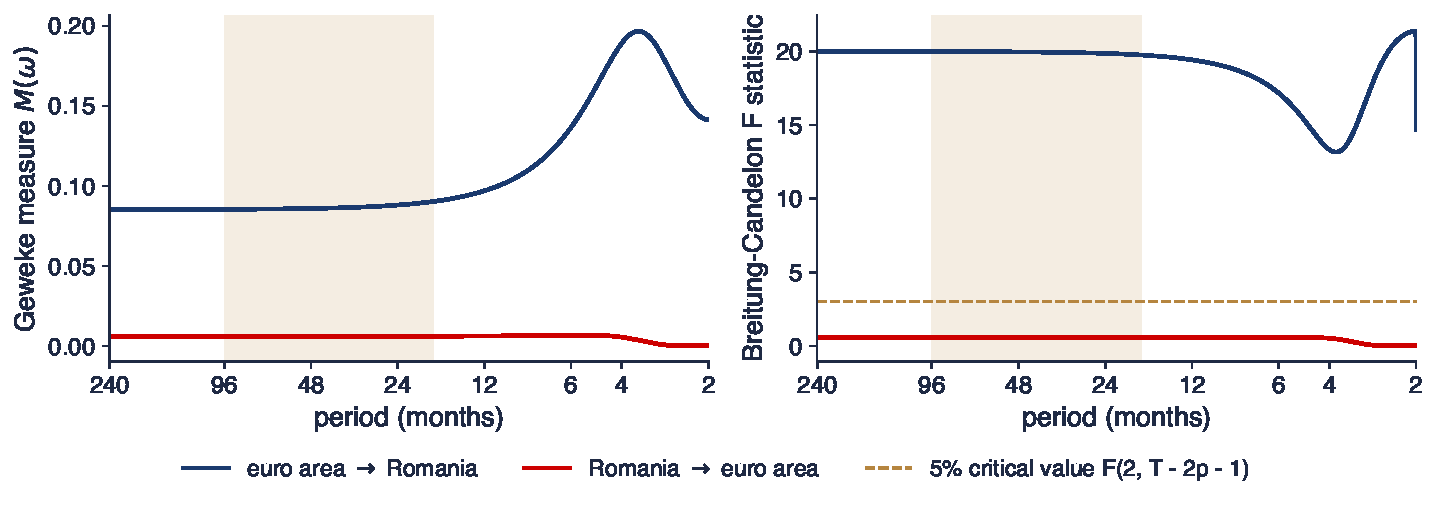
\includegraphics[width=0.97\textwidth,height=0.48\textheight,keepaspectratio]{ats_ch11_causality.pdf}
\end{center}
\vspace{-0.25cm}
\begin{itemize}
    \item VAR(3) in monthly industrial production growth (order by AIC, at least 3); left: Geweke measures; right: Breitung--Candelon $F$ with its 5\% critical value 3.03
\end{itemize}
\quantlet{ATS\_ch11\_causality}{\qlurl{ATS_ch11_causality}}
\end{frame}

\begin{frame}{Interpreting frequency-domain causality}
\itemsize{\small}
\begin{itemize}
    \item Euro area $\to$ Romania: total Geweke measure 0.146 (integral of the curve: 0.145); Romania $\to$ euro area: 0.004
    \item The measure is 0.087 in the business-cycle band and 0.168 at periods under 6 months: past euro-area growth predicts Romanian growth mostly at short horizons
    \item The BC test rejects at 100\% of frequencies for euro area $\to$ Romania and at no frequency in the other direction
    \item A small open economy follows its main market, not the reverse; the frequency profile says which kind of shock transmits fastest
\end{itemize}
\end{frame}

\begin{frame}{Recap: Two series}
\itemsize{\small}
\begin{itemize}
    \item Coherence is an $R^2$ by frequency; it must be smoothed and tested against $1 - \alpha^{1/(L-1)}$
    \item Phase gives leads and lags, modulo $2\pi$, only where coherence is significant; dynamic correlation keeps the sign
    \item Geweke decomposes Granger causality by frequency; Breitung--Candelon tests it with two linear restrictions
\end{itemize}
\end{frame}


%=============================================================================
\section{Filters and the business cycle}
%=============================================================================

\begin{frame}{Band-pass filters}
\itemsize{\small}
\begin{itemize}
    \item Ideal filter for periods $[p_l, p_u]$: gain 1 on the frequencies $[\omega_1, \omega_2] = [2\pi/p_u, 2\pi/p_l]$, 0 elsewhere; its weights are infinitely many
    \[ b_0 = \frac{\omega_2 - \omega_1}{\pi}, \qquad b_j = \frac{\sin j\omega_2 - \sin j\omega_1}{\pi j}, \quad j = \pm1, \pm2, \dots \]
    \item \refBK: truncate at $K$ lags and add a constant so that $\sum_{j=-K}^Ka_j = 0$
    \begin{itemize}
        \item $a_j$: the adjusted weights; the zero sum removes a unit root and a linear trend; symmetric, no phase shift
        \item quarterly recommendation: BK(6, 32, $K = 12$); the price: $K$ observations lost at each end; $a_0 = 0.28$
    \end{itemize}
    \item \refCF: minimise $\E[(y^{\mathrm{ideal}}_t - \hat y_t)^2 \mid y_1, \dots, y_n]$ assuming a random walk
    \begin{itemize}
        \item $y^{\mathrm{ideal}}_t$: the ideal band-pass component; asymmetric, time-varying weights that use the whole sample: no lost observations, but phase shifts near the ends
    \end{itemize}
    \item The business-cycle band of 6--32 quarters (1.5--8 years) follows Burns and Mitchell, as adopted by \refBK
\end{itemize}
\end{frame}

\begin{frame}{The Hodrick--Prescott filter}
\itemsize{\footnotesize}
\begin{columns}[T]
\begin{column}{0.27\textwidth}
\centering
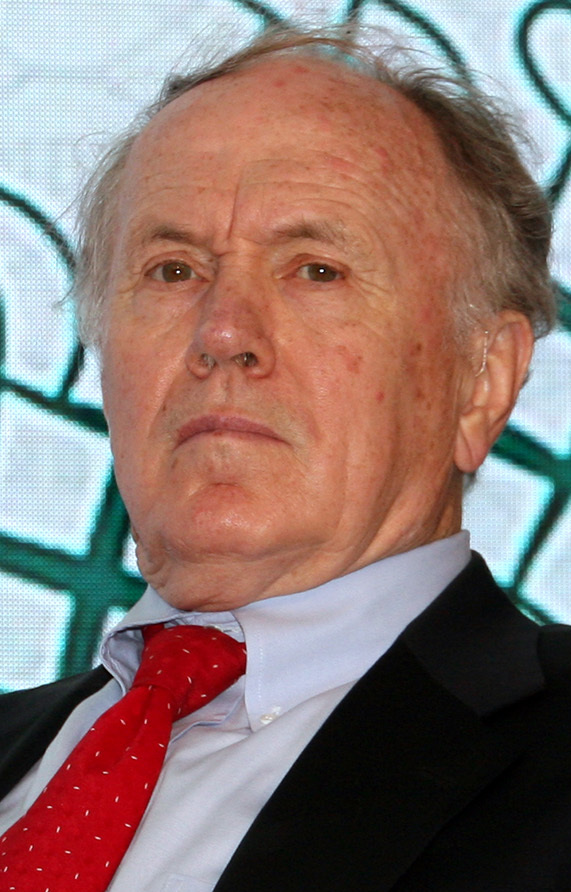
\includegraphics[height=0.4\textheight]{ch11_prescott_2015.jpg}\\[1mm]
\imgcap{Edward C.\ Prescott, 2015}
\imgcredit{https://commons.wikimedia.org/wiki/File:Edward_C_Prescott_2015_(cropped).jpg}{Photo: Narodowy Bank Polski (2015); CC BY-SA 2.0; Wikimedia Commons}
\end{column}
\begin{column}{0.71\textwidth}
\begin{itemize}
    \item \refHP: the trend balances fit against smoothness
    \[ \hat\tau = \arg\min_\tau\sum_t(y_t - \tau_t)^2 + \lambda\sum_t(\Delta^2\tau_t)^2 = (I + \lambda D'D)^{-1}y \]
    \begin{itemize}
        \item $\tau_t$: trend; $\Delta^2\tau_t$: its second difference; $\lambda$: smoothness penalty; $D$: the second-difference matrix; cycle $y_t - \hat\tau_t$
    \end{itemize}
    \item Infinite-sample gain of the cycle: a high-pass filter
    \[ G(\omega) = \frac{4\lambda(1 - \cos\omega)^2}{1 + 4\lambda(1 - \cos\omega)^2} \]
    \begin{itemize}
        \item the Kalman smoother of a local linear trend with signal-to-noise ratio $1/\lambda$ (\atschlink{https://danpele.github.io/Advanced-Time-Series/EN/Courses/chapter6_state_space_models_bayesian_filtering.pdf}{Chapter 6}); $\lambda = 1600$ for quarters; Ravn--Uhlig scaling $\lambda \propto s^4$ ($s$: observations per quarter): 129\,600 for months, 6.25 for years \refRU
    \end{itemize}
\end{itemize}
\end{column}
\end{columns}
\end{frame}

\begin{frame}{Hamilton's critique}
\itemsize{\small}
\begin{itemize}
    \item \refHam: ``why you should never use the HP filter''
    \begin{itemize}
        \item (1) applied to a random walk, HP produces a cycle with dynamics that are artefacts of the filter \refCN
        \item (2) end-of-sample values are very different from the values the same filter gives once more data arrive (one-sided against two-sided)
        \item (3) the $\lambda$ implied by a statistical model fitted to the data is far from 1600
    \end{itemize}
    \item Alternative: the \textbf{regression filter}, the cycle is the error of an $h$-step-ahead regression forecast
    \[ y_{t+h} = \beta_0 + \beta_1y_t + \dots + \beta_py_{t-p+1} + v_{t+h}, \qquad \text{cycle}_{t+h} = \hat v_{t+h} \]
    \begin{itemize}
        \item quarterly $h = 8$, $p = 4$; one-sided by construction; for a random walk $v_{t+h} = y_{t+h} - y_t$
    \end{itemize}
    \item Replies: boosting the HP filter \refPS; a modified Hamilton filter for real time \refQW; the debate is about which gain you want
\end{itemize}
\end{frame}

\begin{frame}{Filters judged by their gain}
\itemsize{\footnotesize}
\begin{center}
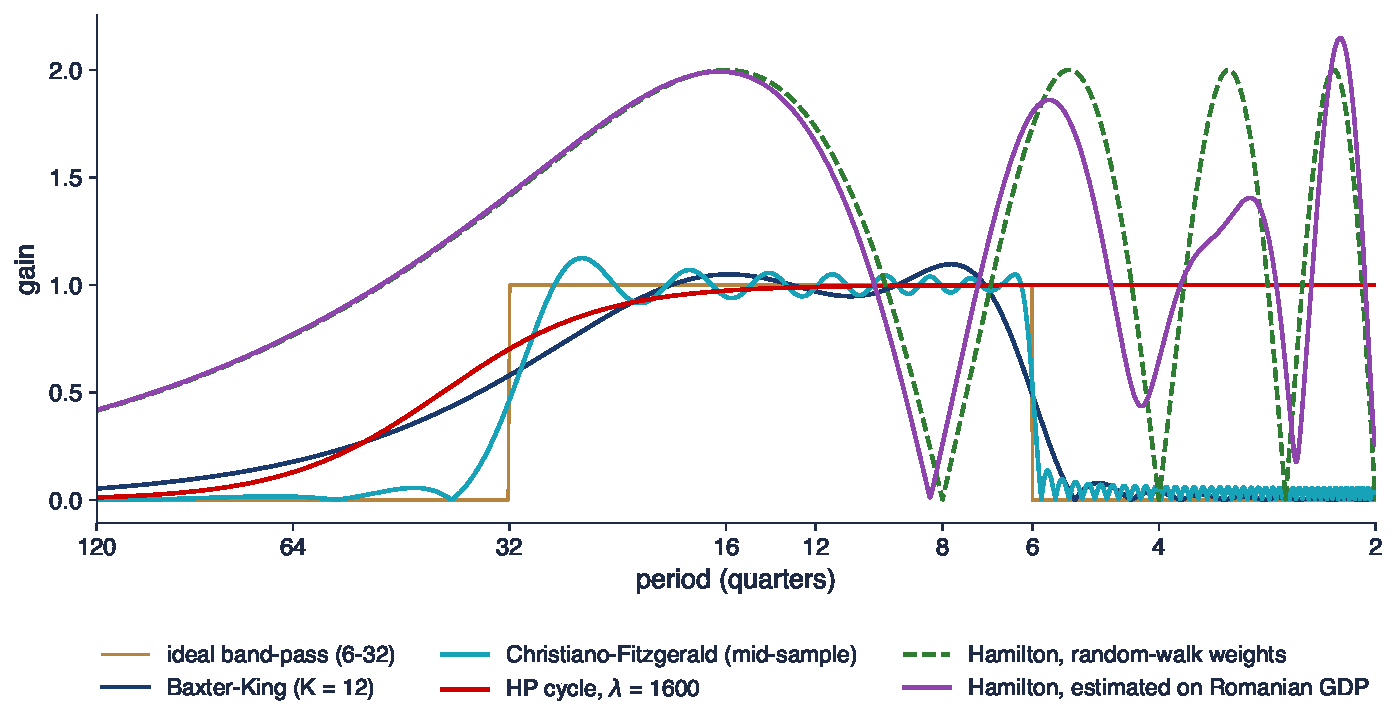
\includegraphics[width=0.97\textwidth,height=0.5\textheight,keepaspectratio]{ats_ch11_gains.pdf}
\end{center}
\vspace{-0.25cm}
\begin{itemize}
    \item Gain from the level to the cycle, by period in quarters; Christiano--Fitzgerald: the weights in the middle of a 126-quarter sample; Hamilton: $h = 8$, $p = 4$
\end{itemize}
\quantlet{ATS\_ch11\_filters}{\qlurl{ATS_ch11_filters}}
\end{frame}

\begin{frame}{Interpreting the gains}
\itemsize{\small}
\begin{itemize}
    \item HP is a high-pass filter: gain 0.70 at 32 quarters, 0.49 at 40 and still 0.16 at 60: the ``HP cycle'' contains cycles longer than 8 years
    \item BK ripples around 1 (maximum 1.10) and lets in 0.41 of the 40-quarter cycle; CF is closer to the ideal shape in mid-sample
    \item Hamilton's filter is not a band-pass: gain 2.00 at 16 quarters and 0.00 at 8 (for random-walk weights); the estimated Romanian weights (sum 0.97) give 1.99 and 0.26
    \item Every filter defines its own cycle: compare cycles only after comparing gains
\end{itemize}
\end{frame}

\begin{frame}{A cycle made by the filter}
\itemsize{\footnotesize}
\begin{center}
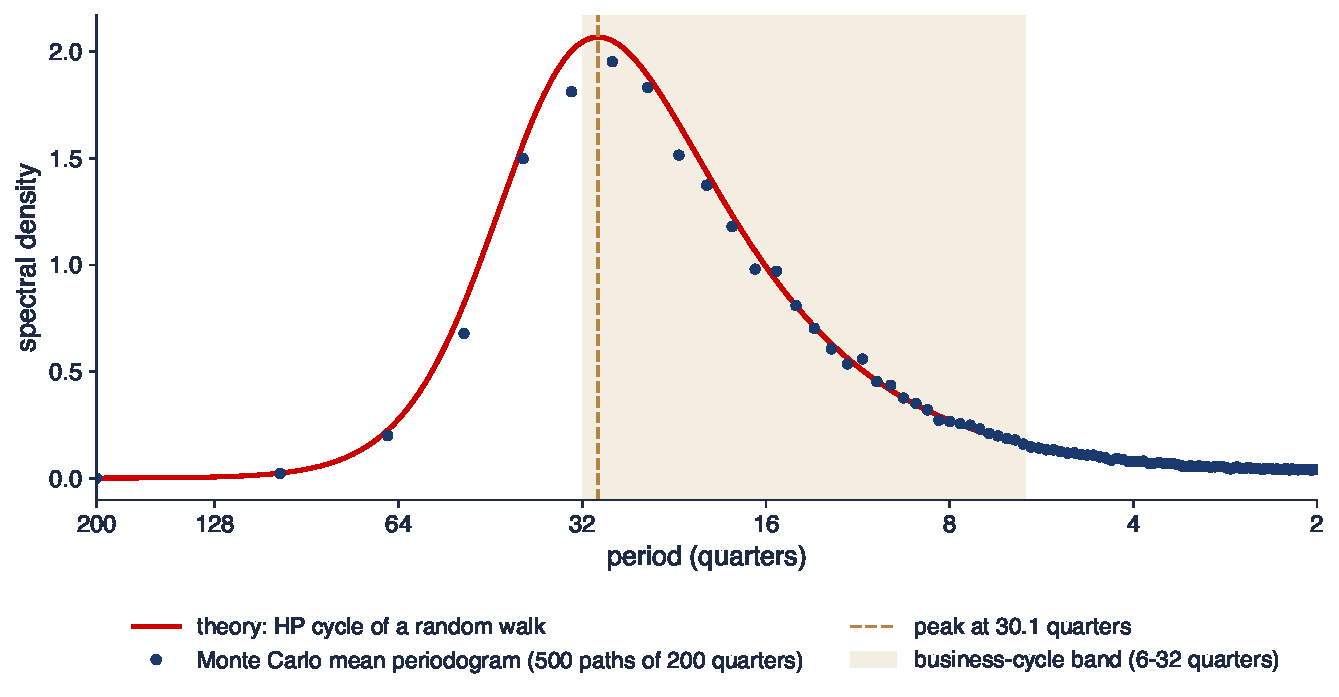
\includegraphics[width=0.97\textwidth,height=0.5\textheight,keepaspectratio]{ats_ch11_cogley_nason.pdf}
\end{center}
\vspace{-0.25cm}
\begin{itemize}
    \item Spectrum of the HP ($\lambda = 1600$) cycle of a random walk: $G(\omega)^2/(2\pi\cdot2(1 - \cos\omega))$, and the average periodogram of HP-filtered simulated random walks
\end{itemize}
\quantlet{ATS\_ch11\_filters}{\qlurl{ATS_ch11_filters}}
\end{frame}

\begin{frame}{Interpreting the spurious cycle}
\itemsize{\small}
\begin{itemize}
    \item A random walk has no cycle, yet its HP cycle peaks at a period of 30.1 quarters (7.5 years); simulation: 28.6
    \item Derivation (Seminar 11, A1): maximise $u^3/(1 + 4\lambda u^2)^2$ in $u = 1 - \cos\omega$: $u^* = \sqrt{3/(4\lambda)}$; replicates \refCN
    \item The peak sits inside the business-cycle band: ``stylised facts'' computed from HP cycles can be properties of the filter
    \item Ravn--Uhlig scaling keeps the peak near 7.5 years at monthly and annual frequency too (Seminar 11, A2)
\end{itemize}
\end{frame}

\begin{frame}{Romanian business cycles by four filters}
\itemsize{\footnotesize}
\begin{center}
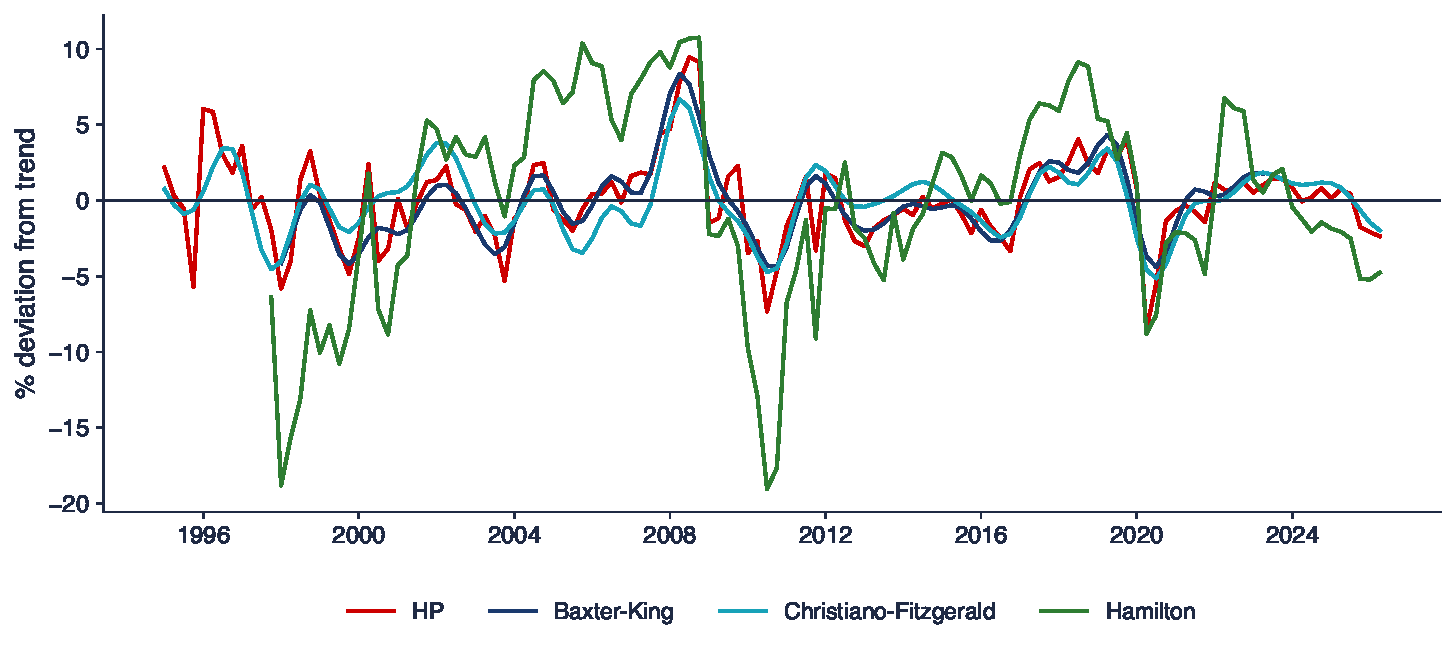
\includegraphics[width=0.97\textwidth,height=0.5\textheight,keepaspectratio]{ats_ch11_ro_cycles.pdf}
\end{center}
\vspace{-0.25cm}
\begin{itemize}
    \item 100 $\times$ log real GDP of Romania, 1995Q1 -- 2026Q2; HP ($\lambda = 1600$), BK(6, 32, 12), CF(6, 32, random walk with drift), Hamilton ($h = 8$, $p = 4$)
\end{itemize}
\quantlet{ATS\_ch11\_filters}{\qlurl{ATS_ch11_filters}}
\end{frame}

\begin{frame}{Interpreting the Romanian cycles}
\itemsize{\footnotesize}
\begin{itemize}
    \item All four place the 2008 peak (HP 9.5\%, BK 8.4\%) and the trough of 2010Q3 (HP \ensuremath{-}7.3\%, BK \ensuremath{-}4.4\%) at the same time
    \item Amplitudes differ: standard deviation HP 2.9, BK 2.5, CF 2.2, Hamilton 6.6; the Hamilton cycle is an 8-quarter forecast error, with a trough of \ensuremath{-}19.0\%
    \item Correlations: BK--HP 0.84, BK--CF 0.84, HP--Hamilton 0.69, CF--Hamilton 0.49
    \item Today's position is uncertain: HP \ensuremath{-}2.4\%, CF \ensuremath{-}2.0\%, Hamilton \ensuremath{-}4.8\% in 2026Q2; BK stops at 2023Q2
\end{itemize}
\end{frame}

\begin{frame}{The end-point problem}
\itemsize{\footnotesize}
\begin{center}
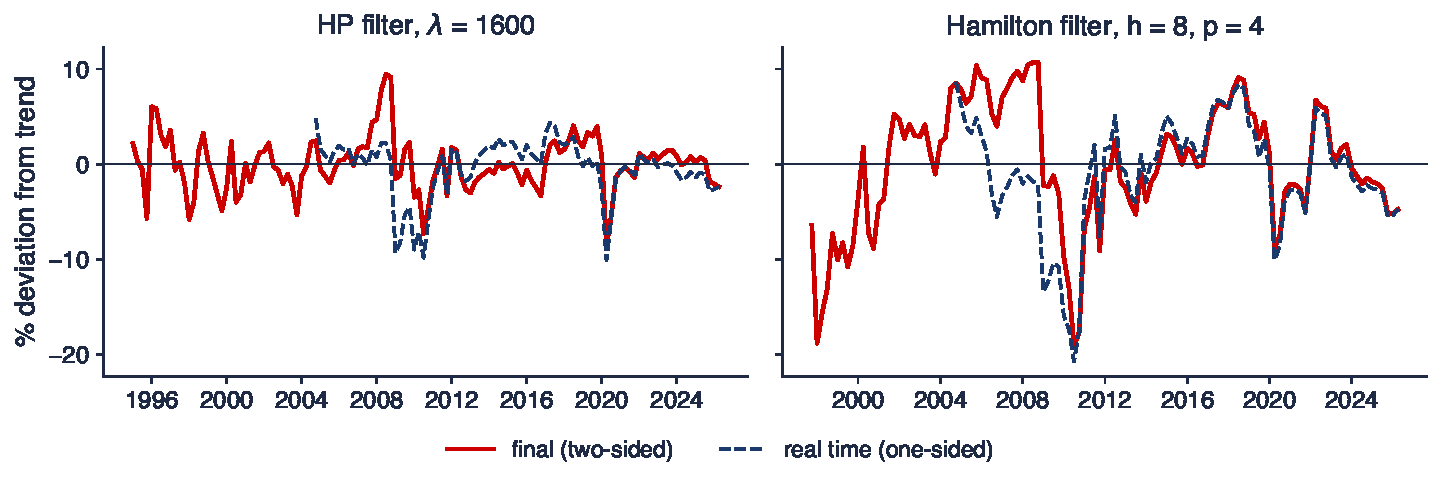
\includegraphics[width=0.97\textwidth,height=0.5\textheight,keepaspectratio]{ats_ch11_endpoint.pdf}
\end{center}
\vspace{-0.25cm}
\begin{itemize}
    \item Romanian GDP: the cycle at each date computed with the data available at that date (real time) and with the full sample (final), from 2004Q4
\end{itemize}
\quantlet{ATS\_ch11\_filters}{\qlurl{ATS_ch11_filters}}
\end{frame}

\begin{frame}{Interpreting the real-time revisions}
\itemsize{\footnotesize}
\begin{itemize}
    \item HP: root mean square revision 2.8 points, as large as the cycle itself (standard deviation 2.8); correlation of real-time and final cycles 0.57; sign wrong in 38\% of quarters
    \item Hamilton: correlation 0.76, sign wrong in 24\% of quarters; but the revision is 4.6 points, because the regression is re-estimated on short samples in a transition economy
    \item The real-time HP filter saw only a small part of the 2008 boom: the output gap that policy needed was the one it measured worst
    \item Report real-time properties of any gap estimate; the final estimate is not information that anyone had
\end{itemize}
\end{frame}

\begin{frame}{Measuring business-cycle synchronisation}
\itemsize{\small}
\begin{itemize}
    \item Correlation of filtered cycles; it depends on the filter (gain) and on a few large episodes
    \item \textbf{Concordance} \refHPa: the share of periods in which the two economies are in the same phase
    \[ C = \frac1T\sum_t\big[S_{xt}S_{yt} + (1 - S_{xt})(1 - S_{yt})\big] \]
    \begin{itemize}
        \item $S_{xt} = 1$ if $x$ is in expansion (here: cycle above trend), 0 otherwise; under independence $\E C = p_xp_y + (1 - p_x)(1 - p_y)$, $p_x$, $p_y$: shares of expansion periods
    \end{itemize}
    \item Dynamic correlation over the business-cycle band \refCFR, which needs no filter
    \item Evidence for Central and Eastern Europe: a meta-analysis of 35 publications finds that some countries already had high correlations with the euro area and that the estimation method changes the correlation significantly \refFK
\end{itemize}
\end{frame}

\begin{frame}{Romania and the euro area: synchronisation over time}
\itemsize{\footnotesize}
\begin{center}
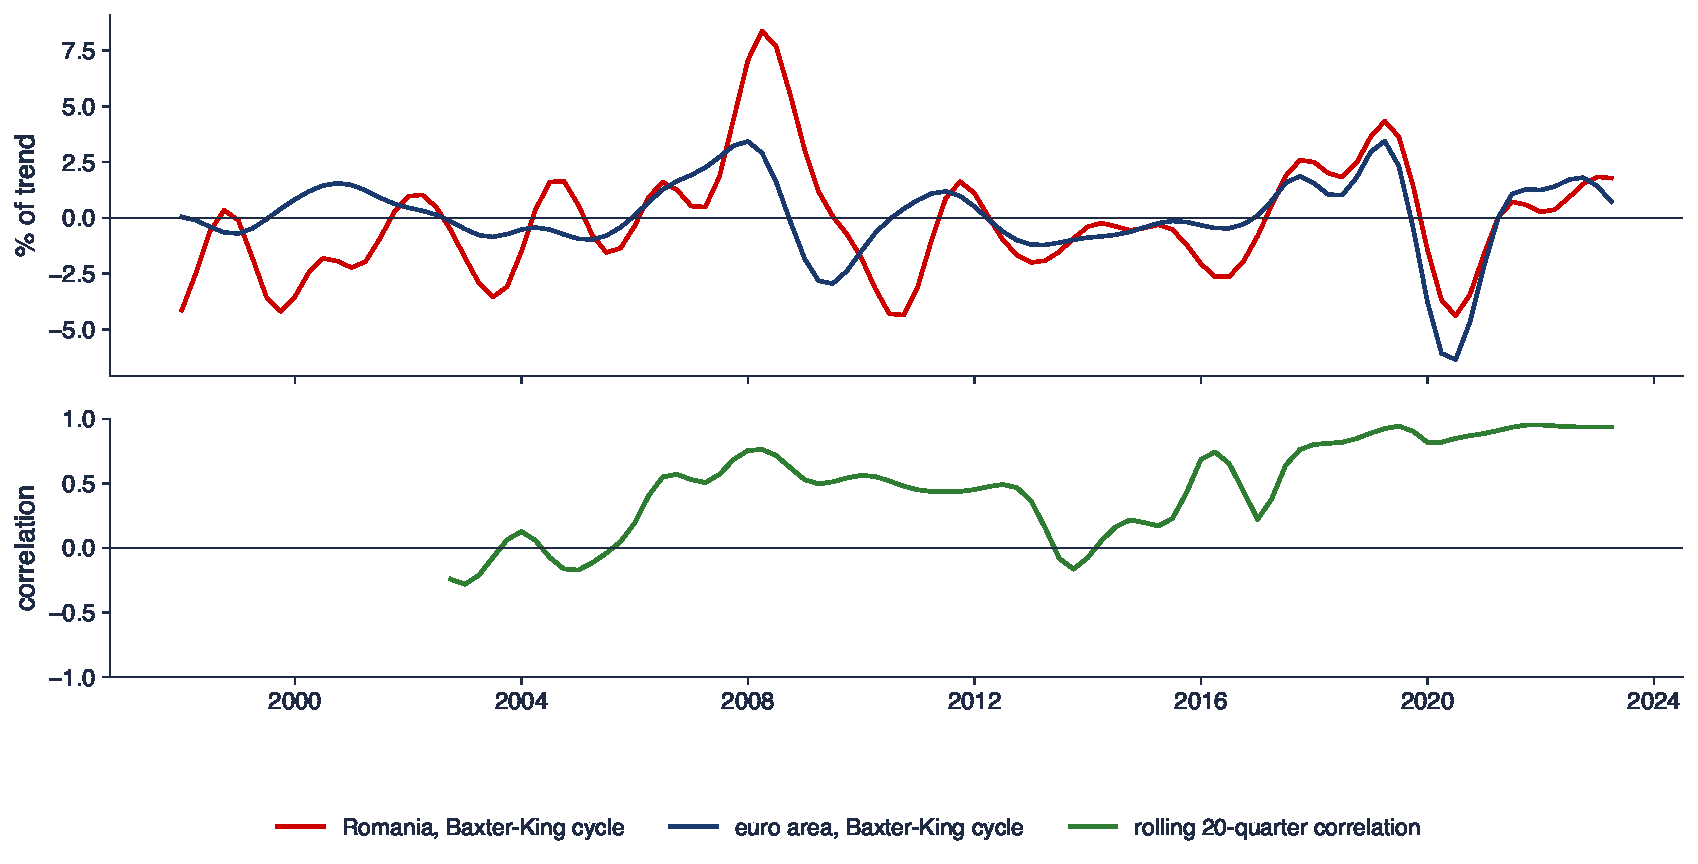
\includegraphics[width=0.97\textwidth,height=0.5\textheight,keepaspectratio]{ats_ch11_sync.pdf}
\end{center}
\vspace{-0.25cm}
\begin{itemize}
    \item Baxter--King cycles of real GDP, 1998Q1 -- 2023Q2, and their rolling 20-quarter correlation
\end{itemize}
\quantlet{ATS\_ch11\_filters}{\qlurl{ATS_ch11_filters}}
\end{frame}

\begin{frame}{Interpreting synchronisation}
\itemsize{\small}
\begin{itemize}
    \item Correlation of the cycles: 0.54 over the whole sample; 0.34 before 2008, 0.47 in 2008--2012, 0.90 in 2013--2019, 0.96 from 2020
    \item Concordance 0.75 against 0.50 under independence: the two economies are above or below trend together most of the time
    \item The Romanian cycle is larger (standard deviation 2.5 against 1.7): synchronised in timing, not in amplitude
    \item The post-2020 correlation is driven by one common shock (the pandemic): a few quarters can make a decade look synchronised
\end{itemize}
\end{frame}

\begin{frame}{Dynamic correlation with the euro area}
\itemsize{\footnotesize}
\begin{center}
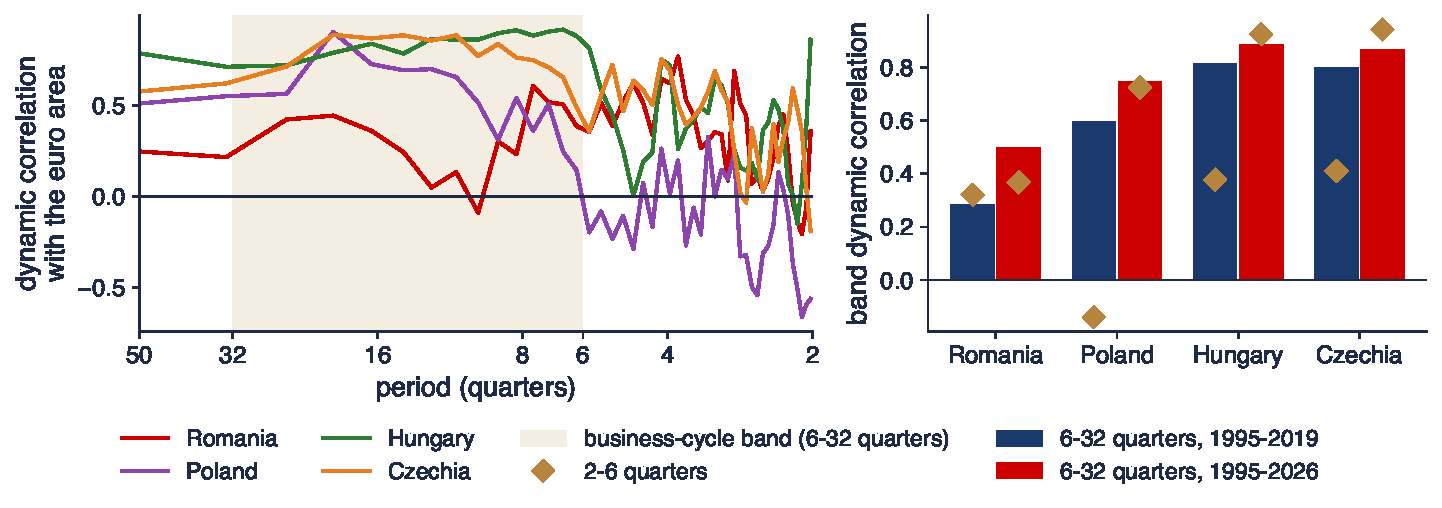
\includegraphics[width=0.97\textwidth,height=0.48\textheight,keepaspectratio]{ats_ch11_dyncorr.pdf}
\end{center}
\vspace{-0.25cm}
\begin{itemize}
    \item Quarterly GDP growth, multitaper $NW = 3$; left: $\rho(\omega)$ for 1995--2019; right: band averages for 6--32 quarters (bars) and 2--6 quarters (diamonds), without and with 2020--2026
\end{itemize}
\quantlet{ATS\_ch11\_cross\_spectrum}{\qlurl{ATS_ch11_cross_spectrum}}
\end{frame}

\begin{frame}{Interpreting the dynamic correlations}
\itemsize{\small}
\begin{itemize}
    \item Before 2020, business-cycle dynamic correlation: Hungary 0.81, Czechia 0.80, Poland 0.60, Romania 0.28
    \item Poland's short-run correlation is \ensuremath{-}0.14: its growth co-moved with the euro area only through the business cycle
    \item With 2020--2026 every number rises (Romania 0.50, Poland 0.75): the pandemic quarter dominates every cross-periodogram
    \item Report synchronisation with and without extreme common shocks; robust (trimmed or rank-based) spectra are a research topic
\end{itemize}
\end{frame}

\begin{frame}{Recap: Filters and the business cycle}
\itemsize{\small}
\begin{itemize}
    \item A cycle is defined by a gain: HP is high-pass, BK and CF approximate a band-pass, Hamilton's regression filter is neither
    \item HP creates a 30-quarter cycle from a random walk and is unreliable in real time
    \item Romania is synchronised with the euro area in timing since 2010, with a larger amplitude
\end{itemize}
\end{frame}


%=============================================================================
\section{Spectra that change over time}
%=============================================================================

\begin{frame}{Evolutionary spectra and local stationarity}
\itemsize{\small}
\begin{itemize}
    \item \refPri: Cramér's representation with a slowly changing amplitude
    \[ X_t = \int A_t(\omega)e^{i\omega t}\,dZ(\omega), \qquad f_t(\omega) = |A_t(\omega)|^2f(\omega) \]
    \begin{itemize}
        \item $A_t(\omega)$: time-varying amplitude; $f_t(\omega)$: the \textbf{evolutionary spectrum} at time $t$
    \end{itemize}
    \item \refDah: \textbf{locally stationary} processes $X_{t,T}$ with $A(t/T, \omega)$ smooth in rescaled time $u = t/T$
    \begin{itemize}
        \item $T$: sample size; a time-varying spectrum $f(u, \omega)$ that can be estimated consistently by a tapered spectrum on a moving window (spectrogram)
    \end{itemize}
    \item \textbf{Uncertainty principle}: a window of length $L$ resolves frequencies only to about $1/L$; long windows blur time, short windows blur frequency
    \item Wavelets (next sections) let the window length change with the frequency: short for high frequencies, long for low ones
\end{itemize}
\end{frame}

\begin{frame}{A spectrum that drifts}
\itemsize{\footnotesize}
\begin{center}
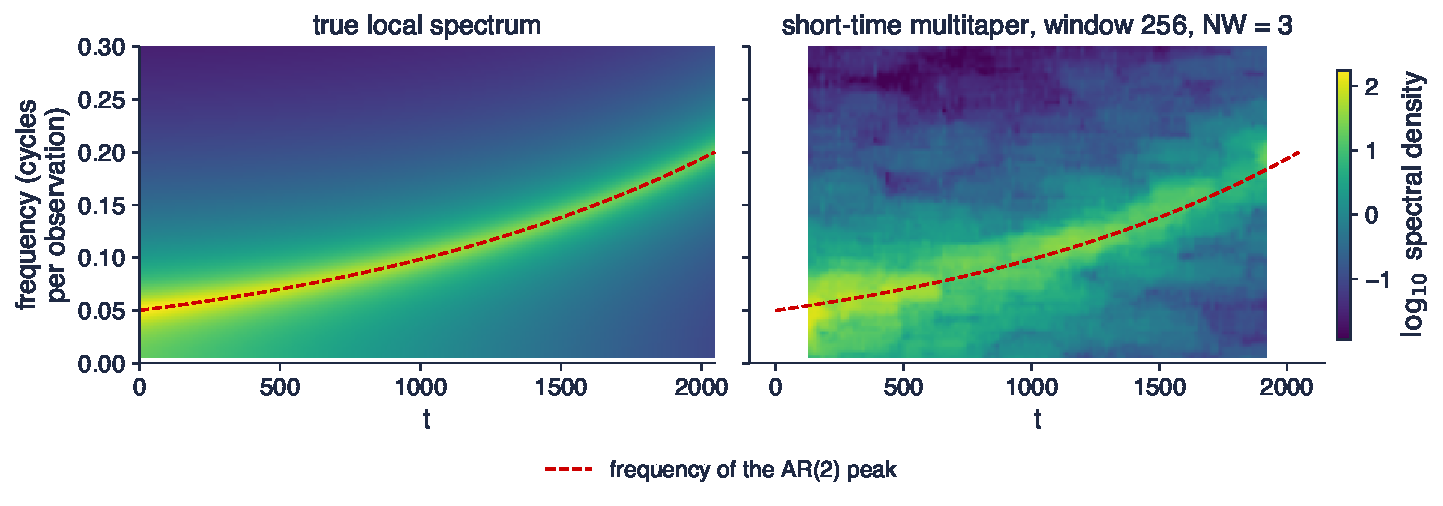
\includegraphics[width=0.97\textwidth,height=0.5\textheight,keepaspectratio]{ats_ch11_spectrogram.pdf}
\end{center}
\vspace{-0.25cm}
\begin{itemize}
    \item $X_t = 2r\cos(\theta_t)X_{t-1} - r^2X_{t-2} + \varepsilon_t$, $r = 0.95$, peak period moving from 20 to 5 over 2048 observations; short-time multitaper on windows of 256 (step 16)
\end{itemize}
\quantlet{ATS\_ch11\_evolutionary}{\qlurl{ATS_ch11_evolutionary}}
\end{frame}

\begin{frame}{Interpreting the spectrogram}
\itemsize{\small}
\begin{itemize}
    \item The spectrogram follows the moving peak: a single spectrum of the whole sample would show a smeared band from 0.05 to 0.2 cycles
    \item Resolution $2NW/L = 0.023$ cycles: fine at high frequencies, coarse for the long periods at the start
    \item The first and last 128 observations have no estimate: every time--frequency method loses the edges (the cone of influence of wavelets)
    \item Economic examples: changing business-cycle length, the shortening of trading cycles, regime changes in volatility
\end{itemize}
\end{frame}

\begin{frame}{Singular spectrum analysis in one slide}
\itemsize{\small}
\begin{itemize}
    \item Embed $x_1, \dots, x_n$ in the $L \times (n - L + 1)$ trajectory (Hankel) matrix $\mathbf X$; SVD $\mathbf X = \sum_i\sigma_i\mathbf u_i\mathbf v_i'$ \refVG
    \item Group eigentriples (trend: slowly varying $\mathbf u_i$; oscillations: pairs with equal $\sigma_i$ and shifted sines) and reconstruct each group by averaging anti-diagonals
    \item Data-adaptive basis instead of fixed sinusoids or wavelets; no model, no stationarity assumption; inference is less developed
    \item A code sketch (\texttt{ssa}) is in the Quantlet engine of this chapter; it is a natural benchmark for wavelet multiresolution
\end{itemize}
\end{frame}

\begin{frame}{Recap: Spectra that change over time}
\itemsize{\small}
\begin{itemize}
    \item Priestley and Dahlhaus give a meaning to a time-varying spectrum
    \item A fixed window trades time against frequency resolution
    \item Wavelets adapt the window to the frequency; SSA adapts the basis to the data
\end{itemize}
\end{frame}


%=============================================================================
\section{Wavelets: decomposition by scale}
%=============================================================================

\begin{frame}{From sinusoids to wavelets}
\itemsize{\footnotesize}
\begin{columns}[T]
\begin{column}{0.28\textwidth}
\centering
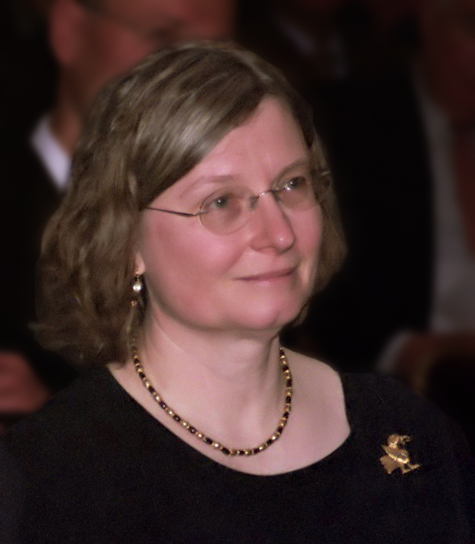
\includegraphics[height=0.36\textheight]{ch11_daubechies_2005.jpg}\\[1mm]
\imgcap{Ingrid Daubechies, 2005}
\imgcredit{https://commons.wikimedia.org/wiki/File:Ingrid_Daubechies_(2005)_(cropped).jpg}{Photo: own work of the uploader (2005); public domain; Wikimedia Commons}
\end{column}
\begin{column}{0.7\textwidth}
\begin{itemize}
    \item A \textbf{wavelet} $\psi$: a short wave, localised in time and frequency \refGM
    \begin{itemize}
        \item $\int\psi = 0$, $\int\psi^2 = 1$; admissible if $C_\psi = \int|\hat\psi(\omega)|^2/|\omega|\,d\omega < \infty$, with $\hat\psi$ the Fourier transform of $\psi$
    \end{itemize}
    \item Continuous wavelet transform (CWT): correlate the series with stretched and shifted copies of $\psi$
    \[ W(s, \tau) = \int x(t)\,\frac{1}{\sqrt s}\,\psi^*\Big(\frac{t - \tau}{s}\Big)dt \]
    \begin{itemize}
        \item $s > 0$: scale (inversely related to frequency); $\tau$: location in time; $\psi^*$: complex conjugate
    \end{itemize}
    \item Compactly supported orthonormal wavelets \refDau{} and the pyramid algorithm \refMal{} give the DWT: $n$ coefficients for $n$ observations; applications: \refCro; \refGSWb; \refACS
\end{itemize}
\end{column}
\end{columns}
\end{frame}

\begin{frame}{DWT, MODWT and multiresolution (1/2)}
\itemsize{\small}
\begin{itemize}
    \item Two filters of length $L$ \refPWb
    \[ \text{scaling (low-pass): } g_l, \qquad \text{wavelet (high-pass): } h_l = (-1)^lg_{L-1-l} \]
    \begin{itemize}
        \item Haar $L = 2$; Daubechies least-asymmetric LA(8) $L = 8$; level $j$ captures periods $[2^j, 2^{j+1}]$: an \textbf{octave} band; $J$ levels plus a smooth
    \end{itemize}
    \item \textbf{MODWT} (maximal overlap DWT): no downsampling, rescaled filters
    \[ \tilde h = h/\sqrt2, \quad \tilde g = g/\sqrt2, \qquad \tilde W_{j,t} = \sum_l\tilde h_{j,l}X_{t-l \bmod n} \]
    \begin{itemize}
        \item $\tilde h_{j,l}$: the level-$j$ wavelet filter; $\tilde W_{j,t}$: wavelet coefficient of level $j$ at time $t$; $\bmod n$: the sample is treated as circular
    \end{itemize}
\end{itemize}
\end{frame}

\begin{frame}{DWT, MODWT and multiresolution (2/2)}
\itemsize{\small}
\begin{itemize}
    \item MODWT properties
    \begin{itemize}
        \item any sample size, shift-invariant (moving the start date does not change the coefficients), $J \times n$ coefficients
        \item energy preserved: $\|X\|^2 = \sum_j\|\tilde W_j\|^2 + \|\tilde V_J\|^2$, with $\tilde V_J$ the scaling (smooth) coefficients
    \end{itemize}
    \item \textbf{Multiresolution analysis (MRA)}: the series is the sum of its details and a smooth
    \[ X_t = \sum_{j=1}^J\mathcal D_{j,t} + \mathcal S_{J,t} \]
    \begin{itemize}
        \item $\mathcal D_j$: the inverse MODWT of level $j$ alone; $\mathcal S_J$: the smooth; zero-phase, aligned with the data
    \end{itemize}
    \item Boundary: the first $L_j - 1 = (2^j - 1)(L - 1)$ coefficients wrap around the sample (circular filtering) and are excluded from estimation
\end{itemize}
\end{frame}

\begin{frame}{Wavelet filters and the Morlet wavelet}
\itemsize{\footnotesize}
\begin{center}
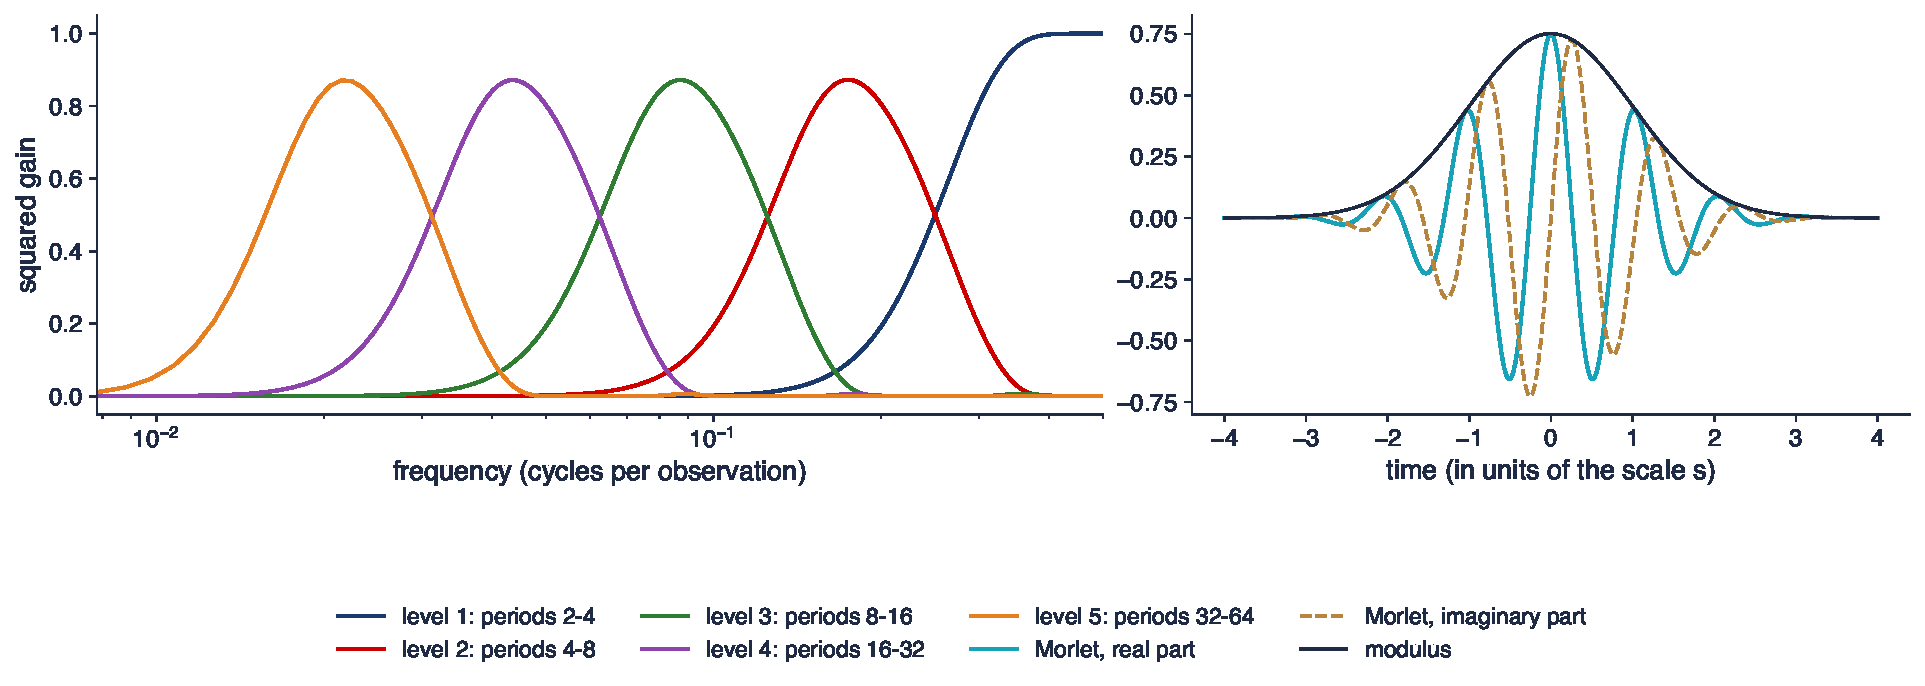
\includegraphics[width=0.97\textwidth,height=0.48\textheight,keepaspectratio]{ats_ch11_wavelets.pdf}
\end{center}
\vspace{-0.25cm}
\begin{itemize}
    \item Left: squared gains of the MODWT LA(8) filters of levels 1--5; right: the Morlet wavelet $\psi_0(\eta) = \pi^{-1/4}e^{i\omega_0\eta}e^{-\eta^2/2}$, $\omega_0 = 6$
\end{itemize}
\quantlet{ATS\_ch11\_wavelets}{\qlurl{ATS_ch11_wavelets}}
\end{frame}

\begin{frame}{Interpreting the wavelet filters}
\itemsize{\small}
\begin{itemize}
    \item Each MODWT level is an approximate band-pass filter for one octave; the bands overlap, so leakage between neighbouring levels is part of the design
    \item The bandwidth grows with frequency: fine frequency resolution for long cycles, fine time resolution for short ones
    \item Morlet is complex: its modulus gives amplitude, its argument gives phase; Fourier period $= 1.033\times$ scale for $\omega_0 = 6$
    \item Orthonormal filters (MODWT) serve variance decomposition and correlation by scale; the Morlet CWT serves time--frequency maps and phase
\end{itemize}
\end{frame}

\begin{frame}{The BET return decomposed by scale}
\itemsize{\footnotesize}
\begin{center}
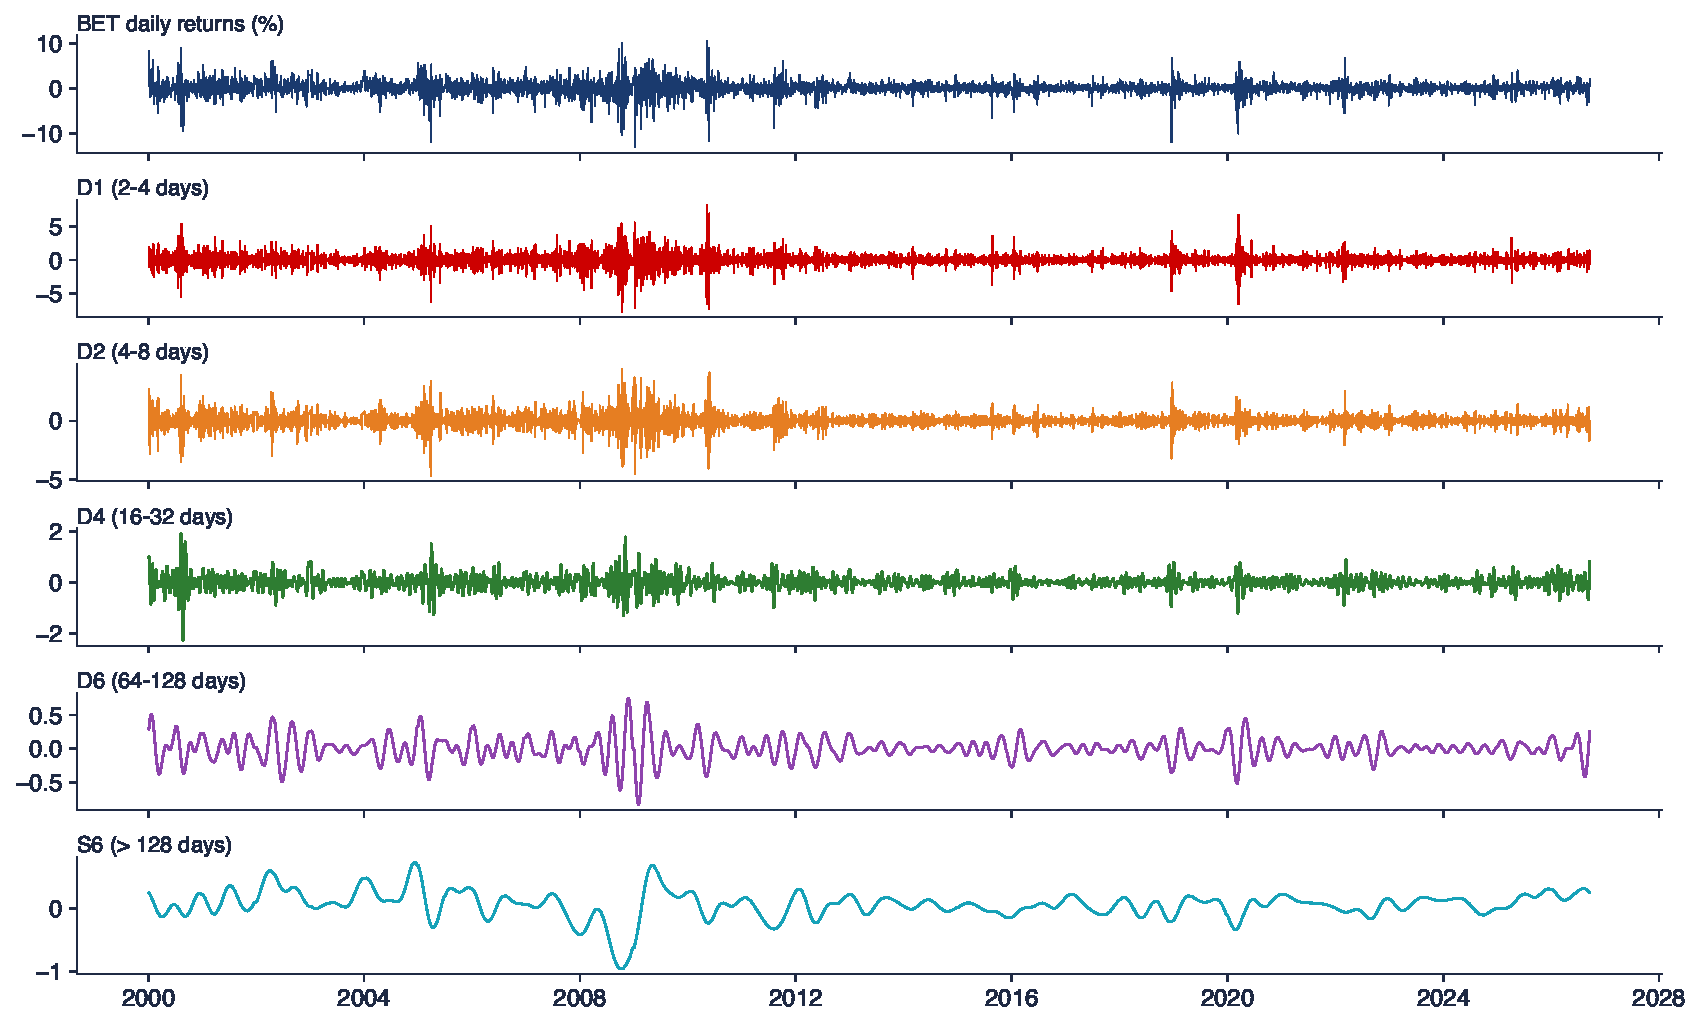
\includegraphics[width=0.97\textwidth,height=0.68\textheight,keepaspectratio]{ats_ch11_mra.pdf}
\end{center}
\vspace{-0.25cm}
\begin{itemize}
    \item MODWT multiresolution analysis, LA(8), $J = 6$, daily BET returns 2000--2026 (6\,670 days); four of the six details and the smooth
\end{itemize}
\quantlet{ATS\_ch11\_wavelets}{\qlurl{ATS_ch11_wavelets}}
\end{frame}

\begin{frame}{Interpreting the multiresolution analysis}
\itemsize{\small}
\begin{itemize}
    \item Energy shares of levels 1--6: 43.0, 26.6, 15.0, 6.8, 3.5, 2.3\%; white noise would give 50.0, 25.0, 12.5, 6.2, 3.1, 1.6\%
    \item Less energy at the shortest scale and more at the longer ones than white noise: positive autocorrelation of BET returns at short horizons
    \item Volatility clustering appears at every scale in 2008 and 2020, but the slow components ($\mathcal D_6$, $\mathcal S_6$) move only in the 2008--2009 crisis
    \item The details add up exactly to the series: a lossless, zero-phase decomposition
\end{itemize}
\end{frame}

\begin{frame}{Wavelet variance, correlation and beta by scale (1/2)}
\itemsize{\small}
\begin{itemize}
    \item \textbf{Wavelet variance}: the variance of the level-$j$ coefficients; the levels add up to the variance of the series \refPer
    \[ \nu_X^2(\tau_j) = \Var\tilde W_{j,t}, \qquad \sum_j\nu^2_X(\tau_j) = \Var X \]
    \begin{itemize}
        \item $\tau_j = 2^{j-1}$: the scale of level $j$; an octave-band version of the spectrum; white noise: $\nu^2(\tau_j) = \sigma^2/2^j$, halving at each level
        \item unbiased estimator: average of $\tilde W^2_{j,t}$ over the $M_j = n - L_j + 1$ non-boundary coefficients; $\eta\hat\nu^2/\nu^2 \approx \chi^2_\eta$, $\eta = \max(M_j/2^j, 1)$ equivalent degrees of freedom
    \end{itemize}
\end{itemize}
\end{frame}

\begin{frame}{Wavelet variance, correlation and beta by scale (2/2)}
\itemsize{\small}
\begin{itemize}
    \item \textbf{Wavelet correlation} \refWGP\ and \textbf{wavelet beta} \refGSW
    \[ \rho_{XY}(\tau_j) = \frac{\Cov(\tilde W^X_j, \tilde W^Y_j)}{\nu_X(\tau_j)\nu_Y(\tau_j)} \]
    \[ \beta(\tau_j) = \frac{\Cov(\tilde W^r_j, \tilde W^m_j)}{\Var\tilde W^m_j} \]
    \begin{itemize}
        \item $\tilde W^r_j$, $\tilde W^m_j$: coefficients of an asset return and of the market return; $\beta(\tau_j)$: systematic risk at the investment horizon $\tau_j$
        \item 95\% interval for the correlation: $\tanh\big(\tanh^{-1}\hat\rho \pm z/\sqrt{M_j/2^j - 3}\big)$, $z = 1.96$
    \end{itemize}
    \item Effective sample size falls by half at each level: long-scale estimates are wide even with 25 years of daily data
\end{itemize}
\end{frame}

\begin{frame}{Wavelet variance of three equity indices}
\itemsize{\footnotesize}
\begin{center}
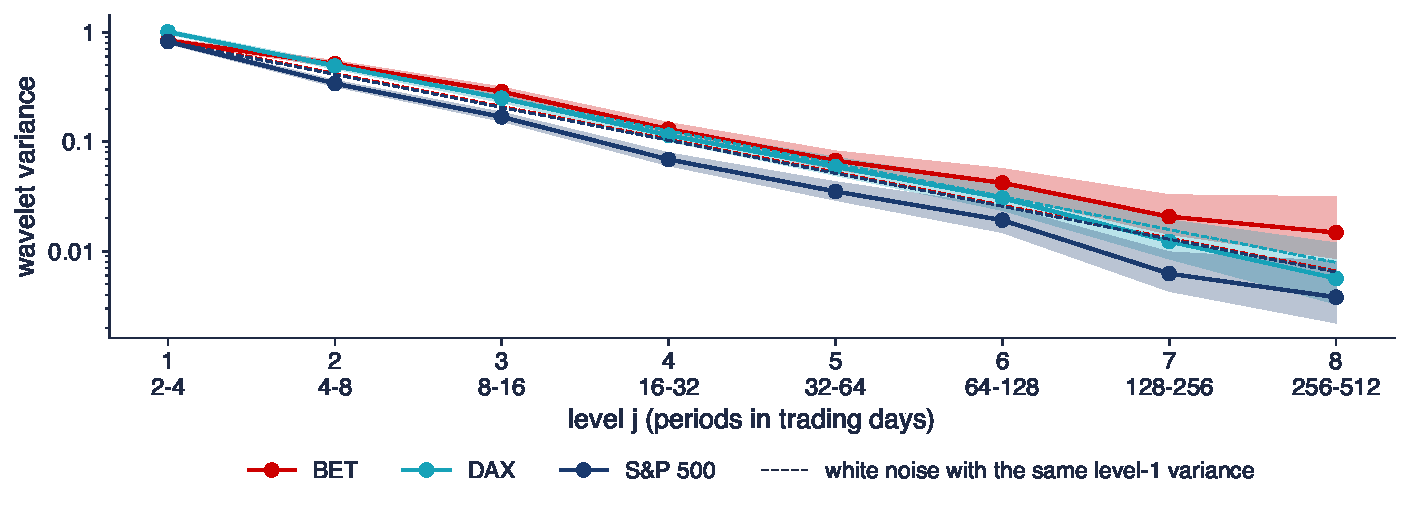
\includegraphics[width=0.97\textwidth,height=0.5\textheight,keepaspectratio]{ats_ch11_wvar.pdf}
\end{center}
\vspace{-0.25cm}
\begin{itemize}
    \item Daily log returns 2000--2026, MODWT LA(8), levels 1--8 with 95\% intervals; dashed: white noise with the same level-1 variance
\end{itemize}
\quantlet{ATS\_ch11\_wavelets}{\qlurl{ATS_ch11_wavelets}}
\end{frame}

\begin{frame}{Interpreting the wavelet variances}
\itemsize{\small}
\begin{itemize}
    \item Ratio of the variance at level 6 (64--128 days) to the white-noise line: BET 1.60, DAX 0.97, S\&P 500 0.75
    \item BET has more long-horizon variance than its daily variance implies (level 8: 2.25): momentum, a thin market; the S\&P 500 has less (0.59): mean reversion of daily moves
    \item This is the variance-ratio test of market efficiency, done scale by scale with valid intervals
    \item Risk measured on daily data and scaled by $\sqrt{h}$ understates BET risk at long horizons
\end{itemize}
\end{frame}

\begin{frame}{Co-movement by scale: BET, DAX and S\&P 500}
\itemsize{\footnotesize}
\begin{center}
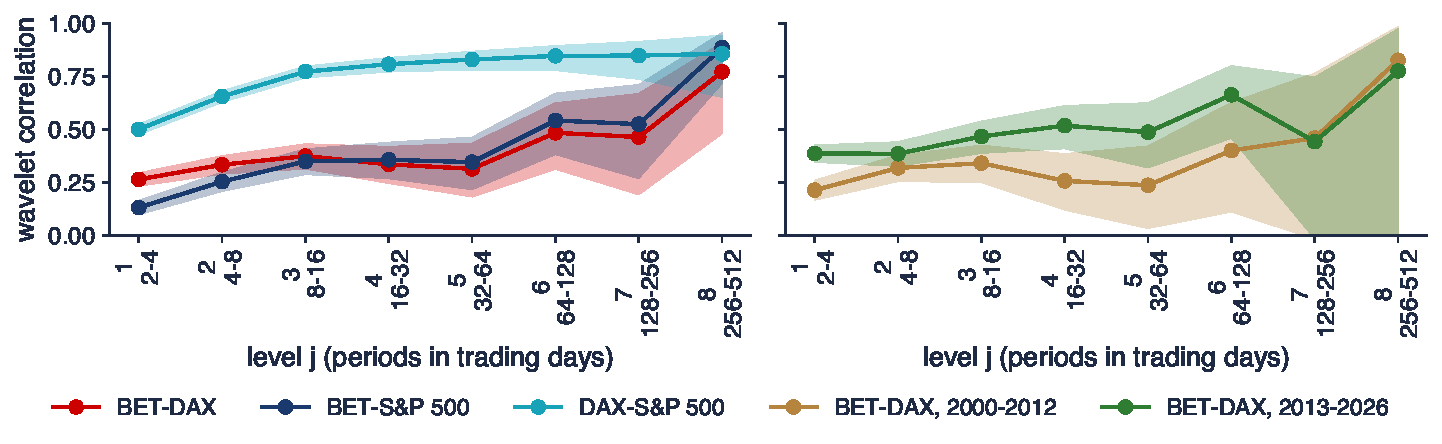
\includegraphics[width=0.97\textwidth,height=0.5\textheight,keepaspectratio]{ats_ch11_wcorr.pdf}
\end{center}
\vspace{-0.25cm}
\begin{itemize}
    \item Daily returns on 6\,433 common trading days, MODWT LA(8); left: three pairs, 2000--2026; right: BET--DAX in two halves; 95\% Fisher-$z$ intervals
\end{itemize}
\quantlet{ATS\_ch11\_wavelets}{\qlurl{ATS_ch11_wavelets}}
\end{frame}

\begin{frame}{Interpreting the wavelet correlations}
\itemsize{\footnotesize}
\begin{itemize}
    \item BET--DAX rises from 0.26 (2--4 days) to 0.77 (256--512 days); the daily correlation (0.31) understates long-run integration
    \item BET--S\&P 500 at level 1 is only 0.13, DAX--S\&P 500 0.50: New York closes after Europe, so daily co-movement shows up a day late; it vanishes at longer scales
    \item BET--DAX at 8--16 days: 0.34 in 2000--2012 against 0.47 in 2013--2026 (level 3): integration has increased at short and medium scales
    \item Wavelet beta of BET on DAX: 0.24 at level 1, 0.56 at level 6: the diversification benefit of the BET shrinks with the horizon (\refGSW; \refRN)
\end{itemize}
\end{frame}

\begin{frame}{Recap: Wavelets: decomposition by scale}
\itemsize{\small}
\begin{itemize}
    \item The MODWT splits variance and covariance into octave bands, for any $n$ and without phase shift
    \item Wavelet variance is a scale-by-scale variance-ratio test; wavelet correlation and beta show integration by horizon
    \item Drop boundary coefficients and use equivalent degrees of freedom for intervals
\end{itemize}
\end{frame}


%=============================================================================
\section{Time--frequency co-movement: wavelet coherence}
%=============================================================================

\begin{frame}{The Morlet transform and its significance (1/2)}
\itemsize{\small}
\begin{itemize}
    \item \refTC: the CWT computed by FFT on a grid of scales
    \[ W_n(s) = \sum_k\hat x_k\,\hat\psi^*(s\omega_k)\,e^{i\omega_kn\delta t}, \qquad s_j = s_02^{j\delta j} \]
    \begin{itemize}
        \item $\hat x_k$: the DFT of the series at frequency $\omega_k$; $\hat\psi$: the Fourier transform of the Morlet wavelet; $\delta t$: time step; $s_0$: smallest scale; $\delta j$: scale step in octaves
        \item wavelet power $|W_n(s)|^2$: the variance of the series at time $n$ and scale $s$
    \end{itemize}
    \item \textbf{Cone of influence} (COI): where the wavelet at scale $s$ reaches the edge, within $\sqrt2\,s$ of either end
    \begin{itemize}
        \item results inside the COI are biased and are not interpreted
    \end{itemize}
\end{itemize}
\end{frame}

\begin{frame}{The Morlet transform and its significance (2/2)}
\itemsize{\small}
\begin{itemize}
    \item Null of red noise, an AR(1) with lag-1 autocorrelation $a$: the power is a scaled $\chi^2_2$
    \[ \frac{|W_n(s)|^2}{\sigma^2} \sim P_k\,\frac{\chi^2_2}{2}, \qquad P_k = \frac{1 - a^2}{1 + a^2 - 2a\cos(2\pi k/N)} \]
    \begin{itemize}
        \item $\sigma^2$: variance of the series; $P_k$: the red-noise spectrum at the Fourier index $k$ matching scale $s$; $N$: number of observations
    \end{itemize}
    \item Global wavelet spectrum: the time average of the power, a smoothed Fourier spectrum
    \[ \bar W^2(s) = \frac1n\sum_n|W_n(s)|^2, \qquad \nu = 2\sqrt{1 + \Big(\frac{n\delta t}{2.32\,s}\Big)^2} \ \text{degrees of freedom} \]
    \item Rectify the power by $1/s$ when comparing scales \refLLW; the pointwise test runs at thousands of points: expect 5\% false patches \refMK
\end{itemize}
\end{frame}

\begin{frame}{Wavelet power of the BET}
\itemsize{\footnotesize}
\begin{center}
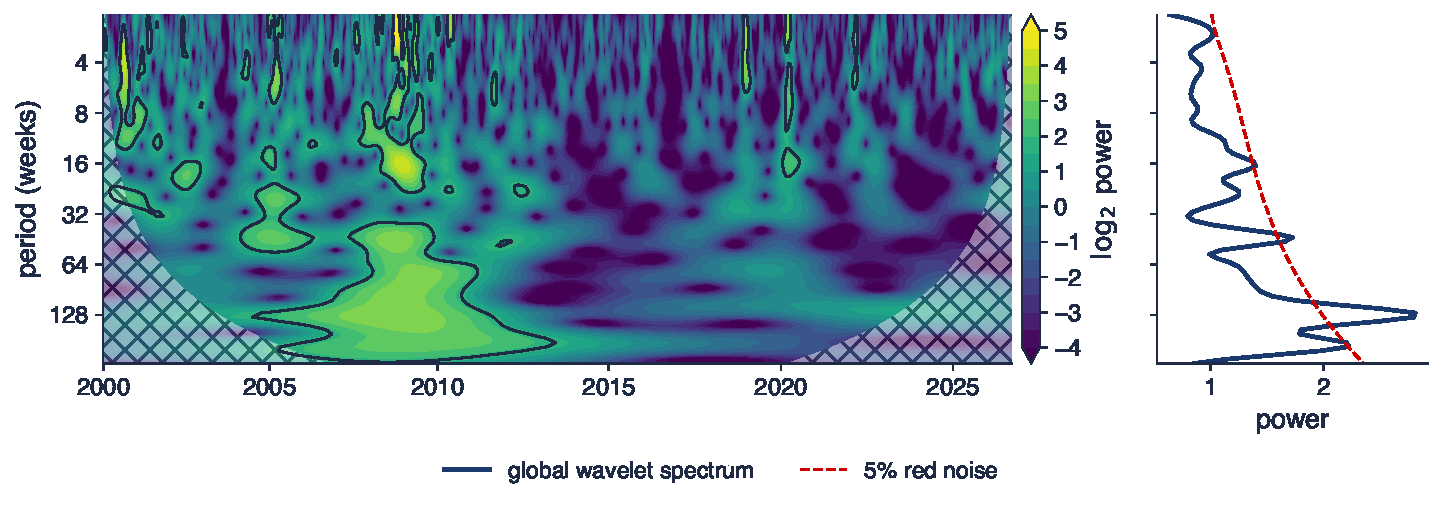
\includegraphics[width=0.97\textwidth,height=0.48\textheight,keepaspectratio]{ats_ch11_cwt_bet.pdf}
\end{center}
\vspace{-0.25cm}
\begin{itemize}
    \item Weekly BET returns (standardised), 1\,379 weeks 2000--2026, Morlet $\omega_0 = 6$, $\delta j = 1/12$; black contours: 5\% red-noise test; hatched: cone of influence; right: global wavelet spectrum
\end{itemize}
\quantlet{ATS\_ch11\_wavelet\_coherence}{\qlurl{ATS_ch11_wavelet_coherence}}
\end{frame}

\begin{frame}{Interpreting the wavelet power}
\itemsize{\small}
\begin{itemize}
    \item Maximum power at a period of 2.6 weeks on 17 October 2008: the Lehman weeks; significant power in 2007--2011 at periods of 32 to 128 weeks
    \item Lag-1 autocorrelation 0.04: the red-noise null is almost white; 11\% of the reliable area is significant at 5\%
    \item Power in returns is variance, not a cycle: the map shows when volatility was concentrated at which horizons
    \item The global spectrum stays inside the red-noise band: no persistent cycle in BET returns, as efficiency predicts
\end{itemize}
\end{frame}

\begin{frame}{Wavelet coherence and phase (1/2)}
\itemsize{\small}
\begin{itemize}
    \item Cross-wavelet transform and \textbf{squared wavelet coherence} \refTW, \refGMJ
    \[ W^{xy}_n(s) = W^x_n(s)W^{y*}_n(s) \]
    \[ R^2_n(s) = \frac{|\mathcal S(s^{-1}W^{xy}_n(s))|^2}{\mathcal S(s^{-1}|W^x_n(s)|^2)\,\mathcal S(s^{-1}|W^y_n(s)|^2)} \in [0, 1] \]
    \begin{itemize}
        \item $\mathcal S$: smoothing, Gaussian in time (width $s$) and a boxcar of 0.6 octaves in scale; $R^2_n(s)$: a local $R^2$ at time $n$ and scale $s$
        \item without smoothing $R^2 \equiv 1$, as for the raw coherence: smoothing is what makes it an estimator
    \end{itemize}
\end{itemize}
\end{frame}

\begin{frame}{Wavelet coherence and phase (2/2)}
\itemsize{\small}
\begin{itemize}
    \item Phase $\arg\mathcal S(s^{-1}W^{xy})$, shown as arrows
    \begin{itemize}
        \item right = in phase, left = anti-phase, up = $x$ leads; lead in time = phase $\times$ period$/2\pi$
    \end{itemize}
    \item Significance by \textbf{Monte Carlo} \refGMJ
    \begin{itemize}
        \item simulate pairs of independent AR(1) series with the data's lag-1 autocorrelations; the 95th percentile of $R^2$ at each scale is the 5\% threshold
    \end{itemize}
    \item Extensions: partial and multiple wavelet coherence, phase differences with confidence bands \refACS; monetary policy \refAAS; energy \refVB
\end{itemize}
\end{frame}

\begin{frame}{BET and DAX in time and frequency}
\itemsize{\footnotesize}
\begin{center}
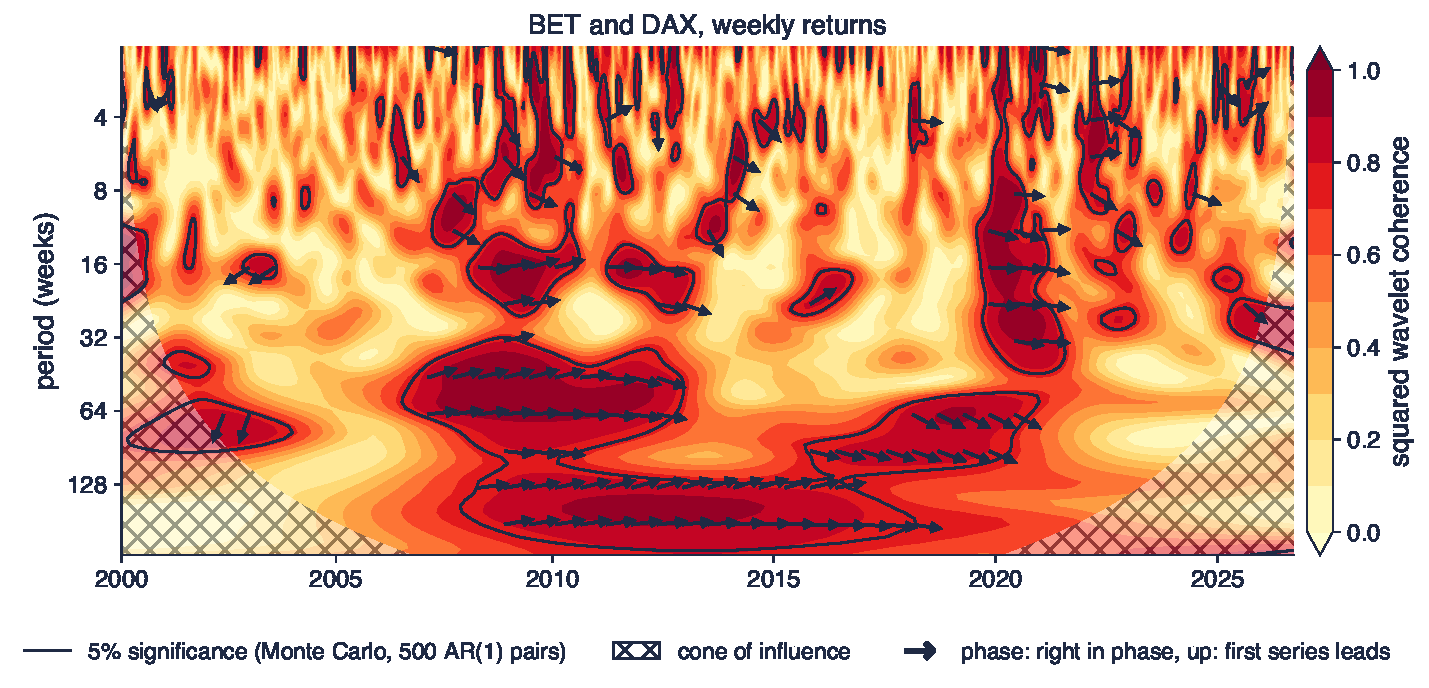
\includegraphics[width=0.97\textwidth,height=0.52\textheight,keepaspectratio]{ats_ch11_wtc_bet_dax.pdf}
\end{center}
\vspace{-0.25cm}
\begin{itemize}
    \item Weekly returns 2000--2026; contours: 5\% significance from 500 AR(1) pairs; arrows only where significant
\end{itemize}
\quantlet{ATS\_ch11\_wavelet\_coherence}{\qlurl{ATS_ch11_wavelet_coherence}}
\end{frame}

\begin{frame}{Interpreting BET--DAX coherence}
\itemsize{\footnotesize}
\begin{itemize}
    \item 23\% of the reliable area is significant (null 95th percentile 7.7\%): the co-movement is real, but concentrated
    \item Average $R^2$ at 8--64 weeks: 0.37 in 2000--2006, 0.76 in 2008--2009, 0.36 in 2014--2019, 0.77 in 2020--June 2021
    \item Phase near zero in crises (0.03 rad in 2008--2009), negative before 2007 (\ensuremath{-}0.97 rad): the DAX led the BET by weeks when the Bucharest market was young
    \item Crises raise coherence: is it contagion or only higher volatility? Correlations rise mechanically with volatility \refFR, and so does $R^2$
\end{itemize}
\end{frame}

\begin{frame}{BET and S\&P 500 in time and frequency}
\itemsize{\footnotesize}
\begin{center}
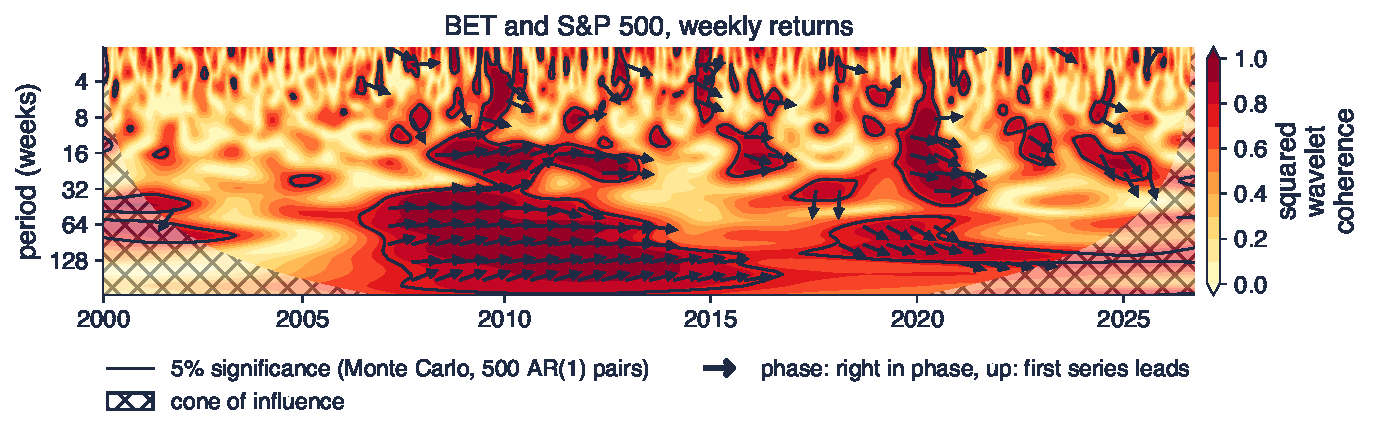
\includegraphics[width=0.97\textwidth,height=0.52\textheight,keepaspectratio]{ats_ch11_wtc_bet_spx.pdf}
\end{center}
\vspace{-0.25cm}
\begin{itemize}
    \item Weekly returns 2000--2026; Monte Carlo significance as before
\end{itemize}
\quantlet{ATS\_ch11\_wavelet\_coherence}{\qlurl{ATS_ch11_wavelet_coherence}}
\end{frame}

\begin{frame}{Interpreting BET--S\&P 500 coherence}
\itemsize{\small}
\begin{itemize}
    \item Significant area 26\% (null 95th percentile 7.7\%); $R^2$ at 8--64 weeks 0.76 in 2008--2009 and 0.48 in 2014--2019
    \item In 2000--2006 the phase is \ensuremath{-}1.24 rad: the S\&P 500 led by about a fifth of the cycle; in crises the markets move in phase
    \item Weekly data remove the one-day lag of the daily wavelet correlation: frequency choice matters for lead--lag claims
    \item Our picture matches the international evidence: co-movement is strongest at low frequencies and in crises \refRN
\end{itemize}
\end{frame}

\begin{frame}{Oil and stocks}
\itemsize{\footnotesize}
\begin{center}
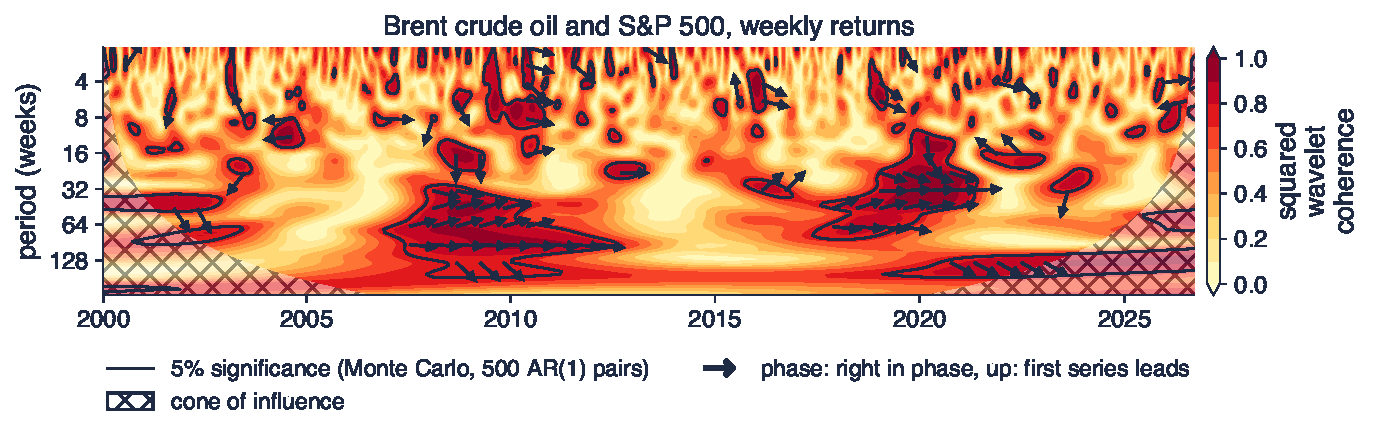
\includegraphics[width=0.97\textwidth,height=0.52\textheight,keepaspectratio]{ats_ch11_wtc_oil.pdf}
\end{center}
\vspace{-0.25cm}
\begin{itemize}
    \item Weekly returns of Brent crude oil (FRED) and the S\&P 500, 2000--2026; Monte Carlo significance from 500 AR(1) pairs
\end{itemize}
\quantlet{ATS\_ch11\_wavelet\_coherence}{\qlurl{ATS_ch11_wavelet_coherence}}
\end{frame}

\begin{frame}{Interpreting oil--stock coherence}
\itemsize{\footnotesize}
\begin{itemize}
    \item Significant area 15\% (null 95th percentile 7.1\%): oil and stocks are linked only in episodes
    \item Before 2007: $R^2$ 0.41 with phase \ensuremath{-}1.86 rad, neither in phase nor in anti-phase: a weak lead--lag link; 2008--2010: 0.70, in phase (\ensuremath{-}0.09 rad): a common demand shock
    \item 2020--2021: 0.58 in phase; 2022--2023: phase \ensuremath{-}2.31 rad, closer to anti-phase: the energy-price shock of the war in Ukraine
    \item The sign of the oil--stock link depends on the type of shock \refKP; wavelet phase shows the switch without identifying it
\end{itemize}
\end{frame}

\begin{frame}{Inflation in Romania and the euro area}
\itemsize{\footnotesize}
\begin{center}
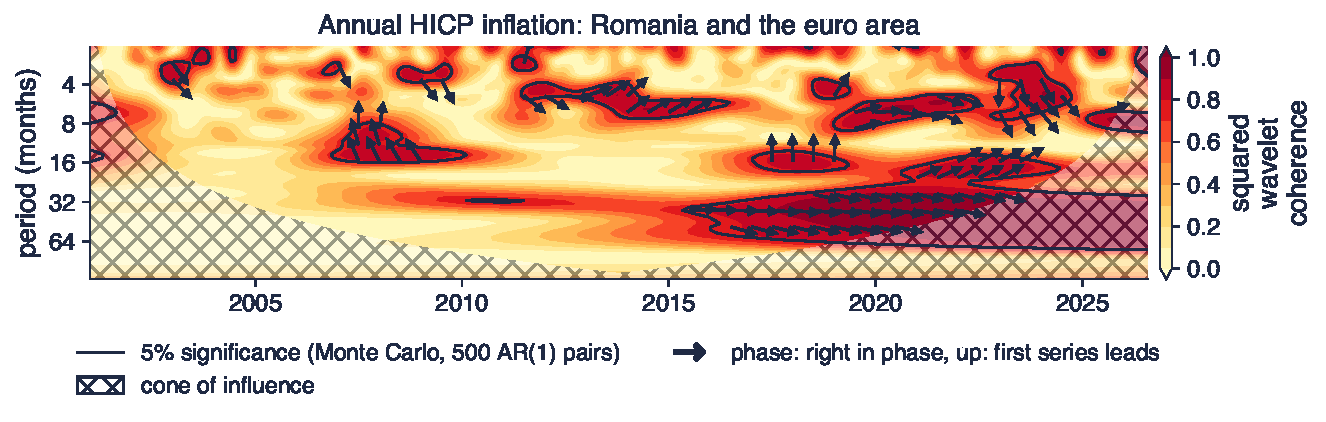
\includegraphics[width=0.97\textwidth,height=0.5\textheight,keepaspectratio]{ats_ch11_wtc_infl_ro.pdf}
\end{center}
\vspace{-0.25cm}
\begin{itemize}
    \item Annual HICP inflation (monthly), January 2001 -- August 2026; Monte Carlo significance against AR(1) pairs with lag-1 autocorrelation 0.97
\end{itemize}
\quantlet{ATS\_ch11\_wavelet\_coherence}{\qlurl{ATS_ch11_wavelet_coherence}}
\end{frame}

\begin{frame}{Interpreting inflation co-movement}
\itemsize{\footnotesize}
\begin{itemize}
    \item Romania--euro area: $R^2$ at 24--64 months 0.23 in 2002--2012, 0.85 from 2015; significant area 17\% (null 95th percentile 8.7\%)
    \item Poland: 0.29 and 0.91; simple correlations 0.34 (Romania) and 0.86 (Poland): Romanian disinflation to 2012 was domestic, the cycle since 2015 is common
    \item 2021--2024 surge, 12--48 months: $R^2$ 0.78, phase 0.14 rad: no detectable lead, a common energy shock
    \item Annual rates overlap twelve months: short periods are smoothed away by construction; only cycles longer than a year are informative
\end{itemize}
\end{frame}

\begin{frame}{Recap: Wavelet coherence}
\itemsize{\small}
\begin{itemize}
    \item Wavelet coherence is a smoothed, time-local coherence; without smoothing it is identically one
    \item Test it by Monte Carlo against AR(1) pairs; read phase only inside significant regions and outside the cone of influence
    \item Equity co-movement peaks in crises and at long horizons; oil--stock phase flips with the type of shock
\end{itemize}
\end{frame}


%=============================================================================
\section{AI for scientific discovery}
%=============================================================================

\begin{frame}{An open question}
\itemsize{\small}
\begin{itemize}
    \item Is the rise of stock-market coherence in crises contagion, or the mechanical effect of higher volatility on a time-local $R^2$?
    \begin{itemize}
        \item formal: $H_0$: the wavelet coherence of BET and DAX in the pre-registered crisis windows equals its value under a model with the same time-varying volatilities and constant dependence
        \item falsified if the crisis coherence exceeds the 95th percentile of a bootstrap from a DCC-GARCH with constant correlation (\atschlink{https://danpele.github.io/Advanced-Time-Series/EN/Courses/chapter8_advanced_volatility.pdf}{Chapter 8}), at pre-registered scales
    \end{itemize}
    \item Why it matters: diversification fails when it is needed; the Forbes--Rigobon correction exists for correlations, not for wavelet coherence
    \begin{itemize}
        \item literature to start from: \refFR, \refRN, \refMK, \refSch, \refACS
    \end{itemize}
\end{itemize}
\end{frame}

\begin{frame}{The discovery loop with an AI assistant}
\itemsize{\footnotesize}
\begin{itemize}
    \item An AI assistant (an LLM such as Claude, ChatGPT, Gemini or Copilot) speeds up each step; Semantic Scholar and Elicit help with the literature
    \begin{itemize}
        \item \textbf{literature}: \aiprompt{List peer-reviewed papers since 2009 that test wavelet coherence between stock markets against a volatility-matched null; give DOIs.} Then check every DOI on Crossref
        \item \textbf{hypothesis}: \aiprompt{Derive the bias of the smoothed wavelet coherence when both series have a common GARCH volatility and constant correlation.}
        \item \textbf{code and replication}: ask for the Grinsted smoothing operator, then reproduce a known case first (two AR(1) series: 5\% significant area)
        \item \textbf{critique}: \aiprompt{Act as a hostile referee: list the ways a significant wavelet-coherence island can arise without any change in dependence.}
    \end{itemize}
    \item Report: what was asked, what was kept, what was rejected (AI\_USE.md, AI\_ERRORS.md)
\end{itemize}
\end{frame}

\begin{frame}{What the human checks}
\itemsize{\small}
\begin{itemize}
    \item Every reference exists and says what is claimed (DOI resolves, title matches, the result is in the paper)
    \item Conventions: angular frequency or cycles, $2\pi$ factors, period $=$ $1.033\times$ scale for Morlet, the sign convention of the phase
    \item Coherence is smoothed; its threshold and the Monte Carlo null are stated; nothing is read inside the cone of influence
    \item Pointwise significance is not areawise significance: count how many islands the null produces
    \item Filters: gain stated; real-time and final cycles separated; results with and without extreme common shocks
\end{itemize}
\end{frame}

\begin{frame}{Mini-case: how many islands does chance produce?}
\itemsize{\footnotesize}
\begin{center}
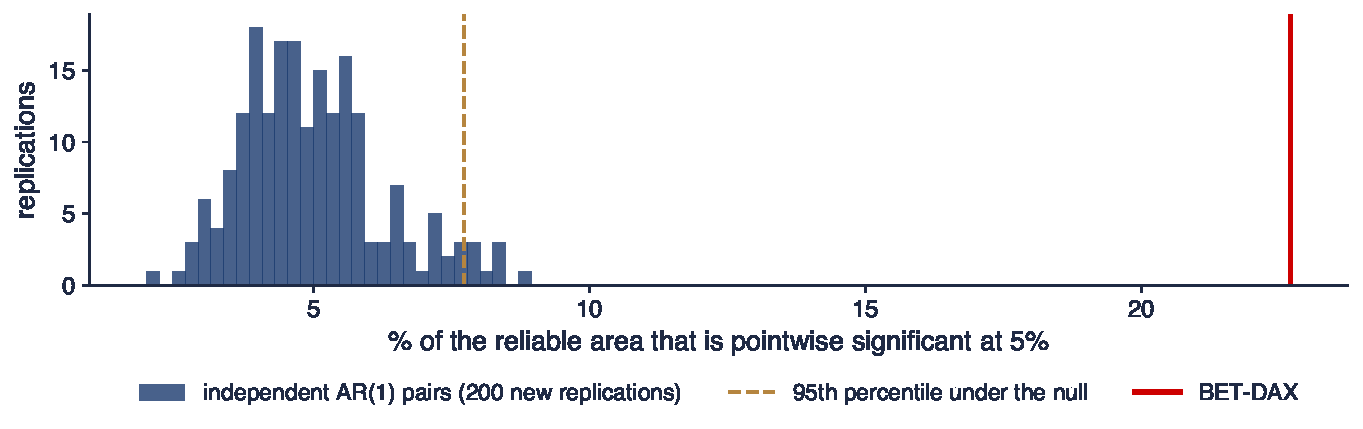
\includegraphics[width=0.97\textwidth,height=0.42\textheight,keepaspectratio]{ats_ch11_ai_case.pdf}
\end{center}
\vspace{-0.25cm}
\begin{itemize}
    \item Share of the reliable time--period area of a wavelet-coherence map that is pointwise significant at 5\%: 200 new pairs of independent AR(1) series with the BET and DAX autocorrelations, and the observed BET--DAX map
    \item Null: mean 5.0\%, 95th percentile 7.7\%, maximum 9.0\%; 100\% of null maps contain significant islands; BET--DAX: 22.7\%. An AI summary that reads every island as a contagion episode is wrong; the overall excess is real
\end{itemize}
\quantlet{ATS\_ch11\_wavelet\_coherence}{\qlurl{ATS_ch11_wavelet_coherence}}
\end{frame}

\begin{frame}{Project idea}
\itemsize{\small}
\begin{itemize}
    \item \textbf{Contagion or volatility? Wavelet coherence of Central and Eastern European stock markets under a volatility-matched null}
    \begin{itemize}
        \item replicate: the Monte Carlo test of \refGMJ{} and the international co-movement maps of \refRN{} on BET, WIG20, BUX, PX against the DAX
        \item extend: a DCC-GARCH bootstrap null (constant dependence, time-varying volatility); areawise tests \refSch; partial coherence controlling for the S\&P 500 \refACS
        \item pre-register: markets, sampling frequency, crisis windows, scales, the null model and the number of replications
    \end{itemize}
    \item Deliverables follow the course rules: repository, report, AI\_USE.md, AI\_ERRORS.md, oral defence
\end{itemize}
\end{frame}


%=============================================================================
\section{Wrap-up}
%=============================================================================

\begin{frame}{Key takeaways}
\itemsize{\small}
\begin{itemize}
    \item The spectrum decomposes variance by frequency; filters act on it through their squared gain
    \item Estimation is a bias--variance choice; multitaper gives low leakage, stable variance and honest bands
    \item Coherence, phase, dynamic correlation and Breitung--Candelon tests describe co-movement and causality by frequency
    \item A business cycle is whatever the filter's gain lets through; HP adds spurious cycles and fails in real time
    \item Wavelets localise variance and co-movement in time and scale; significance needs Monte Carlo and areawise thinking
\end{itemize}
\end{frame}

\begin{frame}{Self-assessment}
\itemsize{\small}
\begin{columns}[T]
\begin{column}{0.56\textwidth}
\begin{block}{Questions}
\begin{itemize}
    \item Why is the periodogram inconsistent although it is asymptotically unbiased?
    \item How does the optimal bandwidth grow with $n$ for a kernel with $q = 2$?
    \item Why is raw (unsmoothed) coherence always equal to one?
    \item Where does the peak of the HP cycle of a random walk come from?
    \item Why is the MODWT preferred to the DWT for wavelet variance?
\end{itemize}
\end{block}
\end{column}
\begin{column}{0.40\textwidth}
\begin{block}{Next: \atschlink{https://danpele.github.io/Advanced-Time-Series/EN/Courses/chapter12_machine_learning_deep_learning.pdf}{Chapter 12}}
\begin{itemize}
    \item Machine learning and deep learning for time series
    \item global models, leakage-free validation, deep architectures
\end{itemize}
\end{block}
\end{column}
\end{columns}
\end{frame}


%=============================================================================
\section{Appendix}
%=============================================================================

\begin{frame}{Appendix: the distribution of the periodogram}
\hypertarget{atsapp1}{}\atsappback{atssrc1}{Back}
\itemsize{\small}
\begin{itemize}
    \item Gaussian white noise: $a_j = \sqrt{2/n}\sum_tx_t\cos(\omega_jt)$, $b_j = \sqrt{2/n}\sum_tx_t\sin(\omega_jt)$ are i.i.d.\ $N(0, \sigma^2)$ for $0 < \omega_j < \pi$ (orthogonality of the Fourier basis)
    \item $I(\omega_j) = (a_j^2 + b_j^2)/(4\pi) = \frac{\sigma^2}{2\pi}\cdot\frac{\chi^2_2}{2}$: mean $f = \sigma^2/(2\pi)$, variance $f^2$, whatever $n$
    \item Linear process: $d_X(\omega_j) = \Psi(e^{-i\omega_j})d_\varepsilon(\omega_j) + o_p(1)$, so $I_X(\omega_j) \approx |\Psi(e^{-i\omega_j})|^2I_\varepsilon(\omega_j) = f(\omega_j)\chi^2_2/2$
    \item Averaging $L$ such ordinates: mean $f$, variance $f^2/L$; this is the logic of every smoothed and multitaper estimator
\end{itemize}
\end{frame}

\begin{frame}{Appendix: two filter facts}
\hypertarget{atsapp2}{}\atsappback{atssrc1}{Back}
\itemsize{\small}
\begin{itemize}
    \item \textbf{Coherence is filter-invariant}: $\tilde x = A(L)x$, $\tilde y = B(L)y$ give $f_{\tilde x\tilde y} = A(\omega)\overline{B(\omega)}f_{xy}$, $f_{\tilde x} = |A|^2f_x$, $f_{\tilde y} = |B|^2f_y$, so $\kappa^2_{\tilde x\tilde y} = \kappa^2_{xy}$ where $A, B \ne 0$
    \item The phase changes by $\arg A - \arg B$: prewhitening with different filters shifts the phase; use the same filter on both series
    \item \textbf{HP cycle of a random walk}: $\Delta y = \varepsilon$, so $f_c(\omega) = G(\omega)^2\sigma^2/(2\pi\cdot2(1 - \cos\omega))$; with $u = 1 - \cos\omega$ this is proportional to $u^3/(1 + 4\lambda u^2)^2$
    \item Setting the derivative to zero: $3(1 + 4\lambda u^2) = 16\lambda u^2$, so $u^* = \sqrt{3/(4\lambda)}$ and the period $2\pi/\arccos(1 - u^*)$
\end{itemize}
\end{frame}


%=============================================================================
\section{References}
%=============================================================================

\begin{frame}{References (1/3)}
\itemsize{\tiny}
\begin{itemize}
    \item Aguiar-Conraria, L., Azevedo, N., \& Soares, M. J. (2008). Using wavelets to decompose the time--frequency effects of monetary policy. \textit{Physica A}, 387(12), 2863--2878. \href{https://doi.org/10.1016/j.physa.2008.01.063}{doi:10.1016/j.physa.2008.01.063}
    \item Aguiar-Conraria, L., \& Soares, M. J. (2014). The continuous wavelet transform: Moving beyond uni- and bivariate analysis. \textit{Journal of Economic Surveys}, 28(2), 344--375. \href{https://doi.org/10.1111/joes.12012}{doi:10.1111/joes.12012}
    \item Andrews, D. W. K. (1991). Heteroskedasticity and autocorrelation consistent covariance matrix estimation. \textit{Econometrica}, 59(3), 817--858. \href{https://doi.org/10.2307/2938229}{doi:10.2307/2938229}
    \item Baxter, M., \& King, R. G. (1999). Measuring business cycles: Approximate band-pass filters for economic time series. \textit{Review of Economics and Statistics}, 81(4), 575--593. \href{https://doi.org/10.1162/003465399558454}{doi:10.1162/003465399558454}
    \item Breitung, J., \& Candelon, B. (2006). Testing for short- and long-run causality: A frequency-domain approach. \textit{Journal of Econometrics}, 132(2), 363--378. \href{https://doi.org/10.1016/j.jeconom.2005.02.004}{doi:10.1016/j.jeconom.2005.02.004}
    \item Brockwell, P. J., \& Davis, R. A. (1991). \textit{Time Series: Theory and Methods} (2nd ed.). Springer. \href{https://doi.org/10.1007/978-1-4419-0320-4}{doi:10.1007/978-1-4419-0320-4}
    \item Christiano, L. J., \& Fitzgerald, T. J. (2003). The band pass filter. \textit{International Economic Review}, 44(2), 435--465. \href{https://doi.org/10.1111/1468-2354.t01-1-00076}{doi:10.1111/1468-2354.t01-1-00076}
    \item Cogley, T., \& Nason, J. M. (1995). Effects of the Hodrick--Prescott filter on trend and difference stationary time series: Implications for business cycle research. \textit{Journal of Economic Dynamics and Control}, 19(1--2), 253--278. \href{https://doi.org/10.1016/0165-1889(93)00781-X}{doi:10.1016/0165-1889(93)00781-X}
    \item Croux, C., Forni, M., \& Reichlin, L. (2001). A measure of comovement for economic variables: Theory and empirics. \textit{Review of Economics and Statistics}, 83(2), 232--241. \href{https://doi.org/10.1162/00346530151143770}{doi:10.1162/00346530151143770}
    \item Crowley, P. M. (2007). A guide to wavelets for economists. \textit{Journal of Economic Surveys}, 21(2), 207--267. \href{https://doi.org/10.1111/j.1467-6419.2006.00502.x}{doi:10.1111/j.1467-6419.2006.00502.x}
    \item Dahlhaus, R. (1997). Fitting time series models to nonstationary processes. \textit{The Annals of Statistics}, 25(1), 1--37. \href{https://doi.org/10.1214/aos/1034276620}{doi:10.1214/aos/1034276620}
    \item Daubechies, I. (1988). Orthonormal bases of compactly supported wavelets. \textit{Communications on Pure and Applied Mathematics}, 41(7), 909--996. \href{https://doi.org/10.1002/cpa.3160410705}{doi:10.1002/cpa.3160410705}
    \item Fidrmuc, J., \& Korhonen, I. (2006). Meta-analysis of the business cycle correlation between the euro area and the CEECs. \textit{Journal of Comparative Economics}, 34(3), 518--537. \href{https://doi.org/10.1016/j.jce.2006.06.007}{doi:10.1016/j.jce.2006.06.007}
    \item Forbes, K. J., \& Rigobon, R. (2002). No contagion, only interdependence: Measuring stock market comovements. \textit{The Journal of Finance}, 57(5), 2223--2261. \href{https://doi.org/10.1111/0022-1082.00494}{doi:10.1111/0022-1082.00494}
    \item Gençay, R., Selçuk, F., \& Whitcher, B. (2005). Multiscale systematic risk. \textit{Journal of International Money and Finance}, 24(1), 55--70. \href{https://doi.org/10.1016/j.jimonfin.2004.10.003}{doi:10.1016/j.jimonfin.2004.10.003}
    \item Gençay, R., Selçuk, F., \& Whitcher, B. (2002). Wavelets for variance--covariance estimation. In \textit{An Introduction to Wavelets and Other Filtering Methods in Finance and Economics}. Academic Press. \href{https://doi.org/10.1016/B978-012279670-8.50010-0}{doi:10.1016/B978-012279670-8.50010-0}
\end{itemize}
\end{frame}

\begin{frame}{References (2/3)}
\itemsize{\tiny}
\begin{itemize}
    \item Geweke, J. (1982). Measurement of linear dependence and feedback between multiple time series. \textit{Journal of the American Statistical Association}, 77(378), 304--313. \href{https://doi.org/10.1080/01621459.1982.10477803}{doi:10.1080/01621459.1982.10477803}
    \item Granger, C. W. J. (1966). The typical spectral shape of an economic variable. \textit{Econometrica}, 34(1), 150--161. \href{https://doi.org/10.2307/1909859}{doi:10.2307/1909859}
    \item Grinsted, A., Moore, J. C., \& Jevrejeva, S. (2004). Application of the cross wavelet transform and wavelet coherence to geophysical time series. \textit{Nonlinear Processes in Geophysics}, 11(5/6), 561--566. \href{https://doi.org/10.5194/npg-11-561-2004}{doi:10.5194/npg-11-561-2004}
    \item Grossmann, A., \& Morlet, J. (1984). Decomposition of Hardy functions into square integrable wavelets of constant shape. \textit{SIAM Journal on Mathematical Analysis}, 15(4), 723--736. \href{https://doi.org/10.1137/0515056}{doi:10.1137/0515056}
    \item Hamilton, J. D. (2018). Why you should never use the Hodrick--Prescott filter. \textit{The Review of Economics and Statistics}, 100(5), 831--843. \href{https://doi.org/10.1162/rest_a_00706}{doi:10.1162/rest\_a\_00706}
    \item Harding, D., \& Pagan, A. (2002). Dissecting the cycle: A methodological investigation. \textit{Journal of Monetary Economics}, 49(2), 365--381. \href{https://doi.org/10.1016/S0304-3932(01)00108-8}{doi:10.1016/S0304-3932(01)00108-8}
    \item Hodrick, R. J., \& Prescott, E. C. (1997). Postwar U.S. business cycles: An empirical investigation. \textit{Journal of Money, Credit and Banking}, 29(1), 1--16. \href{https://doi.org/10.2307/2953682}{doi:10.2307/2953682}
    \item Hurvich, C. M. (1985). Data-driven choice of a spectrum estimate: Extending the applicability of cross-validation methods. \textit{Journal of the American Statistical Association}, 80(392), 933--940. \href{https://doi.org/10.1080/01621459.1985.10478207}{doi:10.1080/01621459.1985.10478207}
    \item Kilian, L., \& Park, C. (2009). The impact of oil price shocks on the U.S. stock market. \textit{International Economic Review}, 50(4), 1267--1287. \href{https://doi.org/10.1111/j.1468-2354.2009.00568.x}{doi:10.1111/j.1468-2354.2009.00568.x}
    \item Liu, Y., San Liang, X., \& Weisberg, R. H. (2007). Rectification of the bias in the wavelet power spectrum. \textit{Journal of Atmospheric and Oceanic Technology}, 24(12), 2093--2102. \href{https://doi.org/10.1175/2007JTECHO511.1}{doi:10.1175/2007JTECHO511.1}
    \item Mallat, S. G. (1989). A theory for multiresolution signal decomposition: The wavelet representation. \textit{IEEE Transactions on Pattern Analysis and Machine Intelligence}, 11(7), 674--693. \href{https://doi.org/10.1109/34.192463}{doi:10.1109/34.192463}
    \item Maraun, D., \& Kurths, J. (2004). Cross wavelet analysis: Significance testing and pitfalls. \textit{Nonlinear Processes in Geophysics}, 11(4), 505--514. \href{https://doi.org/10.5194/npg-11-505-2004}{doi:10.5194/npg-11-505-2004}
    \item Parzen, E. (1961). Mathematical considerations in the estimation of spectra. \textit{Technometrics}, 3(2), 167--190. \href{https://doi.org/10.1080/00401706.1961.10489939}{doi:10.1080/00401706.1961.10489939}
    \item Percival, D. B. (1995). On estimation of the wavelet variance. \textit{Biometrika}, 82(3), 619--631. \href{https://doi.org/10.1093/biomet/82.3.619}{doi:10.1093/biomet/82.3.619}
    \item Percival, D. B., \& Walden, A. T. (1993). \textit{Spectral Analysis for Physical Applications: Multitaper and Conventional Univariate Techniques}. Cambridge University Press. \href{https://doi.org/10.1017/CBO9780511622762}{doi:10.1017/CBO9780511622762}
    \item Percival, D. B., \& Walden, A. T. (2000). \textit{Wavelet Methods for Time Series Analysis}. Cambridge University Press. \href{https://doi.org/10.1017/CBO9780511841040}{doi:10.1017/CBO9780511841040}
\end{itemize}
\end{frame}

\begin{frame}{References (3/3)}
\itemsize{\tiny}
\begin{itemize}
    \item Petropoulos, F., Apiletti, D., Assimakopoulos, V., Babai, M. Z., et al.\ (2022). Forecasting: Theory and practice. \textit{International Journal of Forecasting}, 38(3), 705--871. \href{https://doi.org/10.1016/j.ijforecast.2021.11.001}{doi:10.1016/j.ijforecast.2021.11.001}
    \item Phillips, P. C. B., \& Shi, Z. (2021). Boosting: Why you can use the HP filter. \textit{International Economic Review}, 62(2), 521--570. \href{https://doi.org/10.1111/iere.12495}{doi:10.1111/iere.12495}
    \item Priestley, M. B. (1965). Evolutionary spectra and non-stationary processes. \textit{Journal of the Royal Statistical Society: Series B}, 27(2), 204--229. \href{https://doi.org/10.1111/j.2517-6161.1965.tb01488.x}{doi:10.1111/j.2517-6161.1965.tb01488.x}
    \item Quast, J., \& Wolters, M. H. (2022). Reliable real-time output gap estimates based on a modified Hamilton filter. \textit{Journal of Business \& Economic Statistics}, 40(1), 152--168. \href{https://doi.org/10.1080/07350015.2020.1784747}{doi:10.1080/07350015.2020.1784747}
    \item Ravn, M. O., \& Uhlig, H. (2002). On adjusting the Hodrick--Prescott filter for the frequency of observations. \textit{Review of Economics and Statistics}, 84(2), 371--376. \href{https://doi.org/10.1162/003465302317411604}{doi:10.1162/003465302317411604}
    \item Riedel, K. S., \& Sidorenko, A. (1995). Minimum bias multiple taper spectral estimation. \textit{IEEE Transactions on Signal Processing}, 43(1), 188--195. \href{https://doi.org/10.1109/78.365298}{doi:10.1109/78.365298}
    \item Rua, A., \& Nunes, L. C. (2009). International comovement of stock market returns: A wavelet analysis. \textit{Journal of Empirical Finance}, 16(4), 632--639. \href{https://doi.org/10.1016/j.jempfin.2009.02.002}{doi:10.1016/j.jempfin.2009.02.002}
    \item Schulte, J. A. (2016). Cumulative areawise testing in wavelet analysis and its application to geophysical time series. \textit{Nonlinear Processes in Geophysics}, 23(1), 45--57. \href{https://doi.org/10.5194/npg-23-45-2016}{doi:10.5194/npg-23-45-2016}
    \item Shumway, R. H., \& Stoffer, D. S. (2017). \textit{Time Series Analysis and Its Applications: With R Examples} (4th ed.). Springer. \href{https://doi.org/10.1007/978-3-319-52452-8}{doi:10.1007/978-3-319-52452-8}
    \item Thomson, D. J. (1982). Spectrum estimation and harmonic analysis. \textit{Proceedings of the IEEE}, 70(9), 1055--1096. \href{https://doi.org/10.1109/PROC.1982.12433}{doi:10.1109/PROC.1982.12433}
    \item Torrence, C., \& Compo, G. P. (1998). A practical guide to wavelet analysis. \textit{Bulletin of the American Meteorological Society}, 79(1), 61--78. \href{https://doi.org/10.1175/1520-0477(1998)079\%3C0061:APGTWA\%3E2.0.CO;2}{doi:10.1175/1520-0477(1998)079\textless{}0061:APGTWA\textgreater{}2.0.CO;2}
    \item Torrence, C., \& Webster, P. J. (1999). Interdecadal changes in the ENSO--monsoon system. \textit{Journal of Climate}, 12(8), 2679--2690. \href{https://doi.org/10.1175/1520-0442(1999)012\%3C2679:ICITEM\%3E2.0.CO;2}{doi:10.1175/1520-0442(1999)012\textless{}2679:ICITEM\textgreater{}2.0.CO;2}
    \item Vacha, L., \& Barunik, J. (2012). Co-movement of energy commodities revisited: Evidence from wavelet coherence analysis. \textit{Energy Economics}, 34(1), 241--247. \href{https://doi.org/10.1016/j.eneco.2011.10.007}{doi:10.1016/j.eneco.2011.10.007}
    \item Vautard, R., \& Ghil, M. (1989). Singular spectrum analysis in nonlinear dynamics, with applications to paleoclimatic time series. \textit{Physica D}, 35(3), 395--424. \href{https://doi.org/10.1016/0167-2789(89)90077-8}{doi:10.1016/0167-2789(89)90077-8}
    \item Welch, P. D. (1967). The use of fast Fourier transform for the estimation of power spectra: A method based on time averaging over short, modified periodograms. \textit{IEEE Transactions on Audio and Electroacoustics}, 15(2), 70--73. \href{https://doi.org/10.1109/TAU.1967.1161901}{doi:10.1109/TAU.1967.1161901}
    \item Whitcher, B., Guttorp, P., \& Percival, D. B. (2000). Wavelet analysis of covariance with application to atmospheric time series. \textit{Journal of Geophysical Research: Atmospheres}, 105(D11), 14941--14962. \href{https://doi.org/10.1029/2000JD900110}{doi:10.1029/2000JD900110}
\end{itemize}
\end{frame}

\end{document}
